% Options for packages loaded elsewhere
\PassOptionsToPackage{unicode}{hyperref}
\PassOptionsToPackage{hyphens}{url}
\PassOptionsToPackage{dvipsnames,svgnames,x11names}{xcolor}
%
\documentclass[
  letterpaper,
  DIV=11,
  numbers=noendperiod]{scrartcl}

\usepackage{amsmath,amssymb}
\usepackage{iftex}
\ifPDFTeX
  \usepackage[T1]{fontenc}
  \usepackage[utf8]{inputenc}
  \usepackage{textcomp} % provide euro and other symbols
\else % if luatex or xetex
  \usepackage{unicode-math}
  \defaultfontfeatures{Scale=MatchLowercase}
  \defaultfontfeatures[\rmfamily]{Ligatures=TeX,Scale=1}
\fi
\usepackage{lmodern}
\ifPDFTeX\else  
    % xetex/luatex font selection
\fi
% Use upquote if available, for straight quotes in verbatim environments
\IfFileExists{upquote.sty}{\usepackage{upquote}}{}
\IfFileExists{microtype.sty}{% use microtype if available
  \usepackage[]{microtype}
  \UseMicrotypeSet[protrusion]{basicmath} % disable protrusion for tt fonts
}{}
\makeatletter
\@ifundefined{KOMAClassName}{% if non-KOMA class
  \IfFileExists{parskip.sty}{%
    \usepackage{parskip}
  }{% else
    \setlength{\parindent}{0pt}
    \setlength{\parskip}{6pt plus 2pt minus 1pt}}
}{% if KOMA class
  \KOMAoptions{parskip=half}}
\makeatother
\usepackage{xcolor}
\setlength{\emergencystretch}{3em} % prevent overfull lines
\setcounter{secnumdepth}{5}
% Make \paragraph and \subparagraph free-standing
\makeatletter
\ifx\paragraph\undefined\else
  \let\oldparagraph\paragraph
  \renewcommand{\paragraph}{
    \@ifstar
      \xxxParagraphStar
      \xxxParagraphNoStar
  }
  \newcommand{\xxxParagraphStar}[1]{\oldparagraph*{#1}\mbox{}}
  \newcommand{\xxxParagraphNoStar}[1]{\oldparagraph{#1}\mbox{}}
\fi
\ifx\subparagraph\undefined\else
  \let\oldsubparagraph\subparagraph
  \renewcommand{\subparagraph}{
    \@ifstar
      \xxxSubParagraphStar
      \xxxSubParagraphNoStar
  }
  \newcommand{\xxxSubParagraphStar}[1]{\oldsubparagraph*{#1}\mbox{}}
  \newcommand{\xxxSubParagraphNoStar}[1]{\oldsubparagraph{#1}\mbox{}}
\fi
\makeatother

\usepackage{color}
\usepackage{fancyvrb}
\newcommand{\VerbBar}{|}
\newcommand{\VERB}{\Verb[commandchars=\\\{\}]}
\DefineVerbatimEnvironment{Highlighting}{Verbatim}{commandchars=\\\{\}}
% Add ',fontsize=\small' for more characters per line
\usepackage{framed}
\definecolor{shadecolor}{RGB}{241,243,245}
\newenvironment{Shaded}{\begin{snugshade}}{\end{snugshade}}
\newcommand{\AlertTok}[1]{\textcolor[rgb]{0.68,0.00,0.00}{#1}}
\newcommand{\AnnotationTok}[1]{\textcolor[rgb]{0.37,0.37,0.37}{#1}}
\newcommand{\AttributeTok}[1]{\textcolor[rgb]{0.40,0.45,0.13}{#1}}
\newcommand{\BaseNTok}[1]{\textcolor[rgb]{0.68,0.00,0.00}{#1}}
\newcommand{\BuiltInTok}[1]{\textcolor[rgb]{0.00,0.23,0.31}{#1}}
\newcommand{\CharTok}[1]{\textcolor[rgb]{0.13,0.47,0.30}{#1}}
\newcommand{\CommentTok}[1]{\textcolor[rgb]{0.37,0.37,0.37}{#1}}
\newcommand{\CommentVarTok}[1]{\textcolor[rgb]{0.37,0.37,0.37}{\textit{#1}}}
\newcommand{\ConstantTok}[1]{\textcolor[rgb]{0.56,0.35,0.01}{#1}}
\newcommand{\ControlFlowTok}[1]{\textcolor[rgb]{0.00,0.23,0.31}{\textbf{#1}}}
\newcommand{\DataTypeTok}[1]{\textcolor[rgb]{0.68,0.00,0.00}{#1}}
\newcommand{\DecValTok}[1]{\textcolor[rgb]{0.68,0.00,0.00}{#1}}
\newcommand{\DocumentationTok}[1]{\textcolor[rgb]{0.37,0.37,0.37}{\textit{#1}}}
\newcommand{\ErrorTok}[1]{\textcolor[rgb]{0.68,0.00,0.00}{#1}}
\newcommand{\ExtensionTok}[1]{\textcolor[rgb]{0.00,0.23,0.31}{#1}}
\newcommand{\FloatTok}[1]{\textcolor[rgb]{0.68,0.00,0.00}{#1}}
\newcommand{\FunctionTok}[1]{\textcolor[rgb]{0.28,0.35,0.67}{#1}}
\newcommand{\ImportTok}[1]{\textcolor[rgb]{0.00,0.46,0.62}{#1}}
\newcommand{\InformationTok}[1]{\textcolor[rgb]{0.37,0.37,0.37}{#1}}
\newcommand{\KeywordTok}[1]{\textcolor[rgb]{0.00,0.23,0.31}{\textbf{#1}}}
\newcommand{\NormalTok}[1]{\textcolor[rgb]{0.00,0.23,0.31}{#1}}
\newcommand{\OperatorTok}[1]{\textcolor[rgb]{0.37,0.37,0.37}{#1}}
\newcommand{\OtherTok}[1]{\textcolor[rgb]{0.00,0.23,0.31}{#1}}
\newcommand{\PreprocessorTok}[1]{\textcolor[rgb]{0.68,0.00,0.00}{#1}}
\newcommand{\RegionMarkerTok}[1]{\textcolor[rgb]{0.00,0.23,0.31}{#1}}
\newcommand{\SpecialCharTok}[1]{\textcolor[rgb]{0.37,0.37,0.37}{#1}}
\newcommand{\SpecialStringTok}[1]{\textcolor[rgb]{0.13,0.47,0.30}{#1}}
\newcommand{\StringTok}[1]{\textcolor[rgb]{0.13,0.47,0.30}{#1}}
\newcommand{\VariableTok}[1]{\textcolor[rgb]{0.07,0.07,0.07}{#1}}
\newcommand{\VerbatimStringTok}[1]{\textcolor[rgb]{0.13,0.47,0.30}{#1}}
\newcommand{\WarningTok}[1]{\textcolor[rgb]{0.37,0.37,0.37}{\textit{#1}}}

\providecommand{\tightlist}{%
  \setlength{\itemsep}{0pt}\setlength{\parskip}{0pt}}\usepackage{longtable,booktabs,array}
\usepackage{calc} % for calculating minipage widths
% Correct order of tables after \paragraph or \subparagraph
\usepackage{etoolbox}
\makeatletter
\patchcmd\longtable{\par}{\if@noskipsec\mbox{}\fi\par}{}{}
\makeatother
% Allow footnotes in longtable head/foot
\IfFileExists{footnotehyper.sty}{\usepackage{footnotehyper}}{\usepackage{footnote}}
\makesavenoteenv{longtable}
\usepackage{graphicx}
\makeatletter
\newsavebox\pandoc@box
\newcommand*\pandocbounded[1]{% scales image to fit in text height/width
  \sbox\pandoc@box{#1}%
  \Gscale@div\@tempa{\textheight}{\dimexpr\ht\pandoc@box+\dp\pandoc@box\relax}%
  \Gscale@div\@tempb{\linewidth}{\wd\pandoc@box}%
  \ifdim\@tempb\p@<\@tempa\p@\let\@tempa\@tempb\fi% select the smaller of both
  \ifdim\@tempa\p@<\p@\scalebox{\@tempa}{\usebox\pandoc@box}%
  \else\usebox{\pandoc@box}%
  \fi%
}
% Set default figure placement to htbp
\def\fps@figure{htbp}
\makeatother

% load packages
\usepackage{geometry}
\usepackage{xcolor}
\usepackage{eso-pic}
\usepackage{fancyhdr}
\usepackage{sectsty}
\usepackage{fontspec}
\usepackage{titlesec}

%% Set page size with a wider right margin
\geometry{a4paper, total={170mm,257mm}, left=20mm, top=20mm, bottom=20mm, right=50mm}

%% Let's define some colours
\definecolor{light}{HTML}{E6E6FA}
\definecolor{highlight}{HTML}{800080}
\definecolor{dark}{HTML}{330033}

%% Let's add the border on the right hand side 
\AddToShipoutPicture{% 
    \AtPageLowerLeft{% 
        \put(\LenToUnit{\dimexpr\paperwidth-3cm},0){% 
            \color{light}\rule{3cm}{\LenToUnit\paperheight}%
          }%
     }%
     % logo
    \AtPageLowerLeft{% start the bar at the bottom right of the page
        \put(\LenToUnit{\dimexpr\paperwidth-2.25cm},27.2cm){% move it to the top right
            \color{light}
\includegraphics[width=1.5cm]{_extensions/nrennie/PrettyPDF/logo.png}
          }%
     }%
}

%% Style the page number
\fancypagestyle{mystyle}{
  \fancyhf{}
  \renewcommand\headrulewidth{0pt}
  \fancyfoot[R]{\thepage}
  \fancyfootoffset{3.5cm}
}
\setlength{\footskip}{20pt}

%% style the chapter/section fonts
\chapterfont{\color{dark}\fontsize{20}{16.8}\selectfont}
\sectionfont{\color{dark}\fontsize{20}{16.8}\selectfont}
\subsectionfont{\color{dark}\fontsize{14}{16.8}\selectfont}
\titleformat{\subsection}
  {\sffamily\Large\bfseries}{\thesection}{1em}{}[{\titlerule[0.8pt]}]
  
% left align title
\makeatletter
\renewcommand{\maketitle}{\bgroup\setlength{\parindent}{0pt}
\begin{flushleft}
  {\sffamily\huge\textbf{\MakeUppercase{\@title}}} \vspace{0.3cm} \newline
  {\Large {\@subtitle}} \newline
  \@author
\end{flushleft}\egroup
}
\makeatother

%% Use some custom fonts
\setsansfont{Ubuntu}[
    Path=_extensions/nrennie/PrettyPDF/Ubuntu/,
    Scale=0.9,
    Extension = .ttf,
    UprightFont=*-Regular,
    BoldFont=*-Bold,
    ItalicFont=*-Italic,
    ]

\setmainfont{Ubuntu}[
    Path=_extensions/nrennie/PrettyPDF/Ubuntu/,
    Scale=0.9,
    Extension = .ttf,
    UprightFont=*-Regular,
    BoldFont=*-Bold,
    ItalicFont=*-Italic,
    ]
\usepackage{booktabs}
\usepackage{caption}
\usepackage{longtable}
\usepackage{colortbl}
\usepackage{array}
\usepackage{anyfontsize}
\usepackage{multirow}
\KOMAoption{captions}{tableheading}
\makeatletter
\@ifpackageloaded{tcolorbox}{}{\usepackage[skins,breakable]{tcolorbox}}
\@ifpackageloaded{fontawesome5}{}{\usepackage{fontawesome5}}
\definecolor{quarto-callout-color}{HTML}{909090}
\definecolor{quarto-callout-note-color}{HTML}{0758E5}
\definecolor{quarto-callout-important-color}{HTML}{CC1914}
\definecolor{quarto-callout-warning-color}{HTML}{EB9113}
\definecolor{quarto-callout-tip-color}{HTML}{00A047}
\definecolor{quarto-callout-caution-color}{HTML}{FC5300}
\definecolor{quarto-callout-color-frame}{HTML}{acacac}
\definecolor{quarto-callout-note-color-frame}{HTML}{4582ec}
\definecolor{quarto-callout-important-color-frame}{HTML}{d9534f}
\definecolor{quarto-callout-warning-color-frame}{HTML}{f0ad4e}
\definecolor{quarto-callout-tip-color-frame}{HTML}{02b875}
\definecolor{quarto-callout-caution-color-frame}{HTML}{fd7e14}
\makeatother
\makeatletter
\@ifpackageloaded{caption}{}{\usepackage{caption}}
\AtBeginDocument{%
\ifdefined\contentsname
  \renewcommand*\contentsname{Table of contents}
\else
  \newcommand\contentsname{Table of contents}
\fi
\ifdefined\listfigurename
  \renewcommand*\listfigurename{List of Figures}
\else
  \newcommand\listfigurename{List of Figures}
\fi
\ifdefined\listtablename
  \renewcommand*\listtablename{List of Tables}
\else
  \newcommand\listtablename{List of Tables}
\fi
\ifdefined\figurename
  \renewcommand*\figurename{Figure}
\else
  \newcommand\figurename{Figure}
\fi
\ifdefined\tablename
  \renewcommand*\tablename{Table}
\else
  \newcommand\tablename{Table}
\fi
}
\@ifpackageloaded{float}{}{\usepackage{float}}
\floatstyle{ruled}
\@ifundefined{c@chapter}{\newfloat{codelisting}{h}{lop}}{\newfloat{codelisting}{h}{lop}[chapter]}
\floatname{codelisting}{Listing}
\newcommand*\listoflistings{\listof{codelisting}{List of Listings}}
\makeatother
\makeatletter
\makeatother
\makeatletter
\@ifpackageloaded{caption}{}{\usepackage{caption}}
\@ifpackageloaded{subcaption}{}{\usepackage{subcaption}}
\makeatother
\makeatletter
\@ifpackageloaded{tcolorbox}{}{\usepackage[skins,breakable]{tcolorbox}}
\makeatother
\makeatletter
\@ifundefined{shadecolor}{\definecolor{shadecolor}{rgb}{.97, .97, .97}}{}
\makeatother
\makeatletter
\@ifundefined{codebgcolor}{\definecolor{codebgcolor}{named}{light}}{}
\makeatother
\makeatletter
\ifdefined\Shaded\renewenvironment{Shaded}{\begin{tcolorbox}[frame hidden, colback={codebgcolor}, breakable, boxrule=0pt, enhanced, sharp corners]}{\end{tcolorbox}}\fi
\makeatother

\usepackage{bookmark}

\IfFileExists{xurl.sty}{\usepackage{xurl}}{} % add URL line breaks if available
\urlstyle{same} % disable monospaced font for URLs
\hypersetup{
  pdftitle={Practical 8},
  colorlinks=true,
  linkcolor={highlight},
  filecolor={Maroon},
  citecolor={Blue},
  urlcolor={highlight},
  pdfcreator={LaTeX via pandoc}}


\title{Practical 8}
\author{}
\date{}

\begin{document}
\maketitle

\pagestyle{mystyle}


\textbf{Aim of this practical:}

In this practical we are going to look at some model comparison and
validation techniques.

\section{Distance Sampling}\label{distance-sampling}

In this practical we will:

\begin{itemize}
\tightlist
\item
  Fit a spatial distance sampling model
\item
  Estimate animal abundance
\item
  Compare models that use different detection functions
\end{itemize}

Libraries to load:

\begin{Shaded}
\begin{Highlighting}[]
\FunctionTok{library}\NormalTok{(dplyr)}
\FunctionTok{library}\NormalTok{(INLA)}
\FunctionTok{library}\NormalTok{(ggplot2)}
\FunctionTok{library}\NormalTok{(patchwork)}
\FunctionTok{library}\NormalTok{(inlabru)     }
\FunctionTok{library}\NormalTok{(sf)}
\CommentTok{\# load some libraries to generate nice map plots}
\FunctionTok{library}\NormalTok{(scico)}
\FunctionTok{library}\NormalTok{(mapview)}
\end{Highlighting}
\end{Shaded}

\subsection{The data}\label{the-data}

In the next exercise, we will explore data from a combination of several
NOAA shipboard surveys conducted on pan-tropical spotted dolphins in the
Gulf of Mexico. The data set is available in \texttt{inlabru}
(originally obtianed from the \texttt{dsm} R package) and contains the
following information:

\begin{itemize}
\item
  A total of 47 observations of groups of dolphins were detected. The
  group size was recorded, as well as the Beaufort sea state at the time
  of the observation.
\item
  Transect width is 16 km, i.e.~maximal detection distance 8 km
  (transect half-width 8 km).
\end{itemize}

We can load and visualize the data as follows:

\begin{Shaded}
\begin{Highlighting}[]
\NormalTok{mexdolphin }\OtherTok{\textless{}{-}}\NormalTok{ mexdolphin\_sf}
\NormalTok{mexdolphin}\SpecialCharTok{$}\NormalTok{depth }\OtherTok{\textless{}{-}}\NormalTok{ mexdolphin}\SpecialCharTok{$}\NormalTok{depth }\SpecialCharTok{\%\textgreater{}\%} \FunctionTok{mutate}\NormalTok{(}\AttributeTok{depth=}\FunctionTok{scale}\NormalTok{(depth)}\SpecialCharTok{\%\textgreater{}\%}\FunctionTok{c}\NormalTok{())}
\FunctionTok{mapviewOptions}\NormalTok{(}\AttributeTok{basemaps =} \FunctionTok{c}\NormalTok{( }\StringTok{"OpenStreetMap.DE"}\NormalTok{))}

\FunctionTok{mapview}\NormalTok{(mexdolphin}\SpecialCharTok{$}\NormalTok{points,}\AttributeTok{zcol=}\StringTok{"size"}\NormalTok{)}\SpecialCharTok{+}
  \FunctionTok{mapview}\NormalTok{(mexdolphin}\SpecialCharTok{$}\NormalTok{samplers)}\SpecialCharTok{+}
 \FunctionTok{mapview}\NormalTok{(mexdolphin}\SpecialCharTok{$}\NormalTok{ppoly )}
\end{Highlighting}
\end{Shaded}

\begin{verbatim}
file:///C:/Users/admin/AppData/Local/Temp/RtmpwbcYDb/filee6bc6e263b9b/widgete6bc4b1e1ae3.html screenshot completed
\end{verbatim}

\pandocbounded{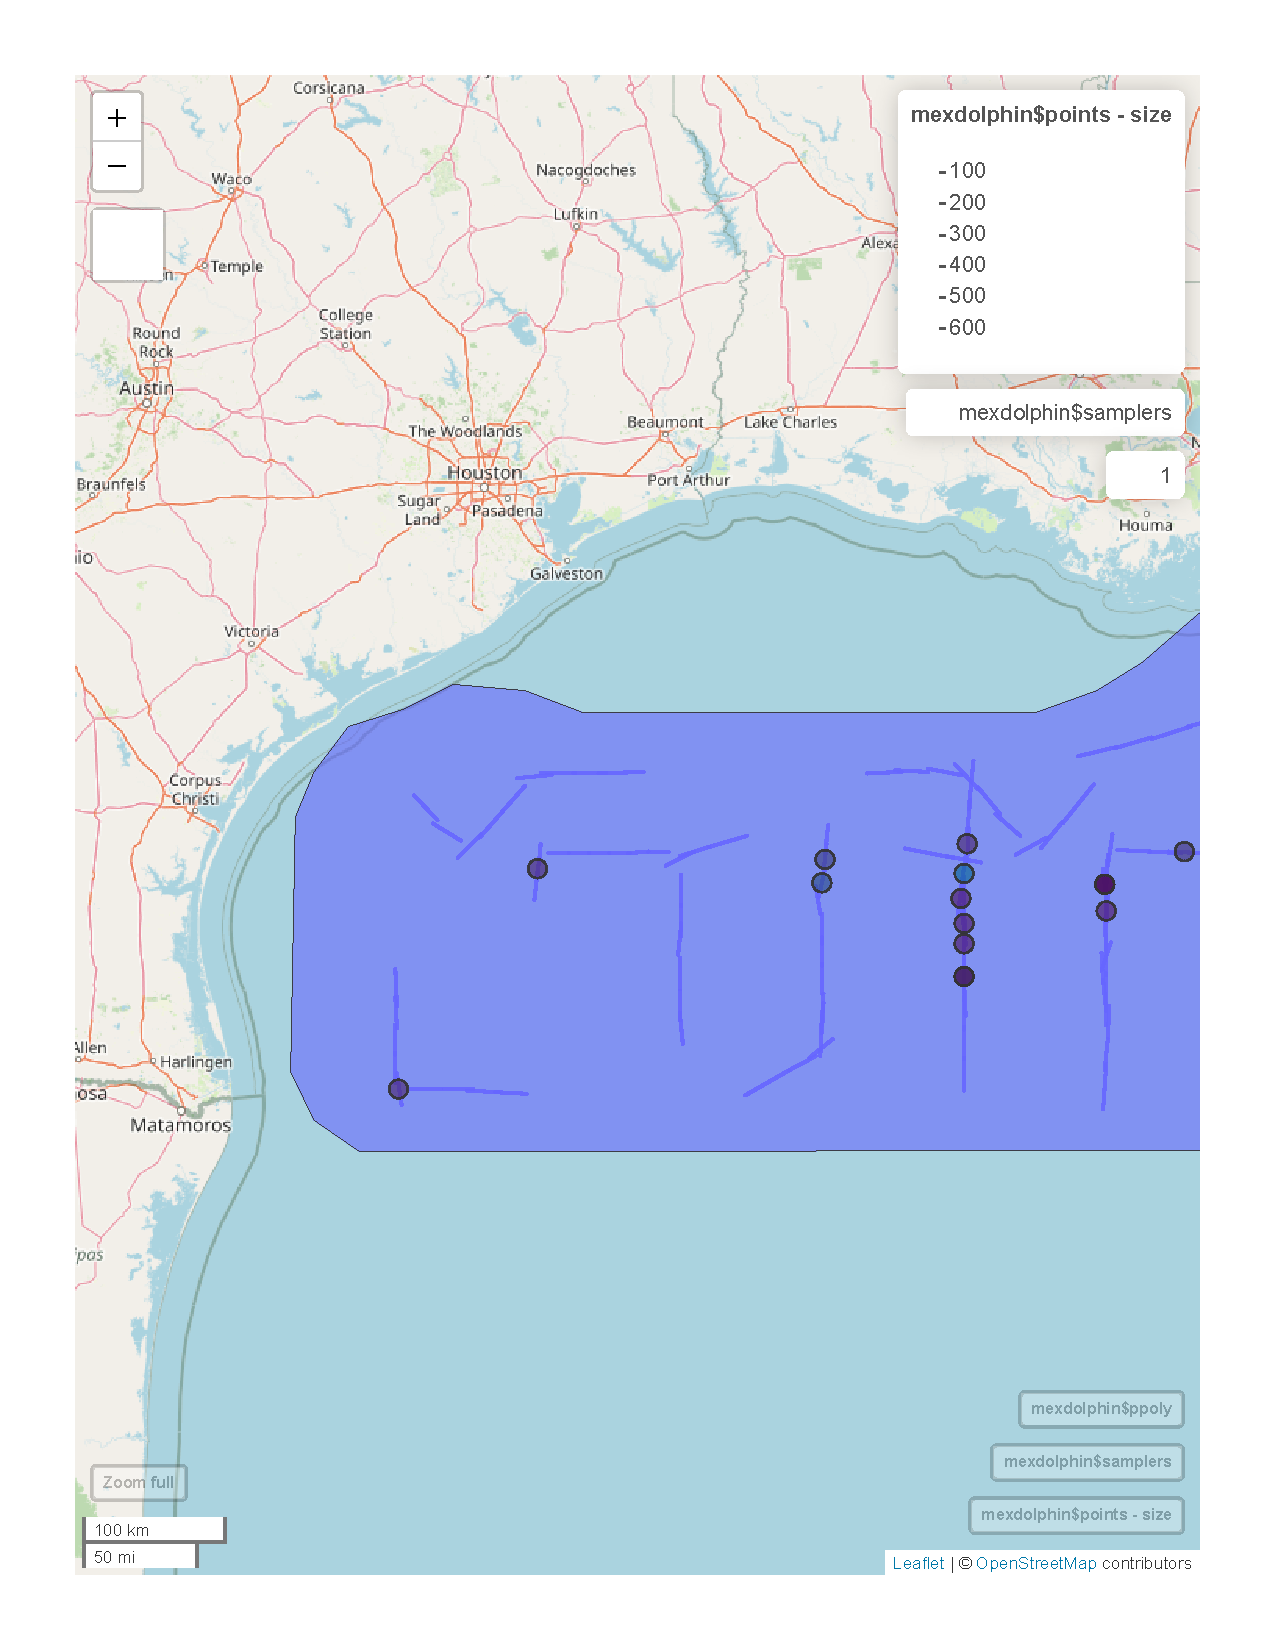
\includegraphics[keepaspectratio]{day5_practical_8_files/figure-pdf/unnamed-chunk-4-1.pdf}}

\subsection{The workflow}\label{the-workflow}

To model the density of spotted dolphins we take a thinned point process
model of the form:

\begin{equation}\phantomsection\label{eq-thinned_pp}{
p(\mathbf{y} | \lambda)  \propto \exp \left( -\int_\Omega \lambda(\mathbf{s}) p(\mathbf{s}) \mathrm{d}\mathbf{s} \right) \prod_{i=1}^n \lambda(\mathbf{s}_i) p(\mathbf{s}_i)) 
}\end{equation}

When fitting a distance sampling model we need to fulfill the following
tasks:

\begin{enumerate}
\def\labelenumi{\arabic{enumi}.}
\item
  Build the mesh
\item
  Define the SPDE representation of the spatial GF. This includes
  defining the priors for the range and sd of the spatial GF
\item
  Define the \emph{components} of the linear predictor. This includes
  the spatial GF and all eventual covariates
\item
  Define the observation model using the \texttt{bru\_obs()} function
\item
  Run the model using the \texttt{bru()} function
\end{enumerate}

\subsubsection{Building the mesh}\label{building-the-mesh}

The first task is to build the mesh that covers the area of interest.
For this purpose we use the function \texttt{fm\_mesh\_2d}. To do so, we
need to define the area of interest. We can either use a predefined
boundary or create a non convex hull surrounding the location of the
specie sightseeings

\subsection{non-covex hull}

\begin{Shaded}
\begin{Highlighting}[]
\NormalTok{boundary0 }\OtherTok{=} \FunctionTok{fm\_nonconvex\_hull}\NormalTok{(mexdolphin}\SpecialCharTok{$}\NormalTok{points,}\AttributeTok{convex =} \SpecialCharTok{{-}}\FloatTok{0.1}\NormalTok{)}

\NormalTok{mesh\_0 }\OtherTok{=} \FunctionTok{fm\_mesh\_2d}\NormalTok{(}\AttributeTok{boundary =}\NormalTok{ boundary0,}
                          \AttributeTok{max.edge =} \FunctionTok{c}\NormalTok{(}\DecValTok{30}\NormalTok{, }\DecValTok{150}\NormalTok{), }\CommentTok{\# The largest allowed triangle edge length.}
                          \AttributeTok{cutoff =} \DecValTok{15}\NormalTok{,}
                          \AttributeTok{crs =} \FunctionTok{fm\_crs}\NormalTok{(mexdolphin}\SpecialCharTok{$}\NormalTok{points))}
\FunctionTok{ggplot}\NormalTok{() }\SpecialCharTok{+} \FunctionTok{gg}\NormalTok{(mesh\_0)}
\end{Highlighting}
\end{Shaded}

\pandocbounded{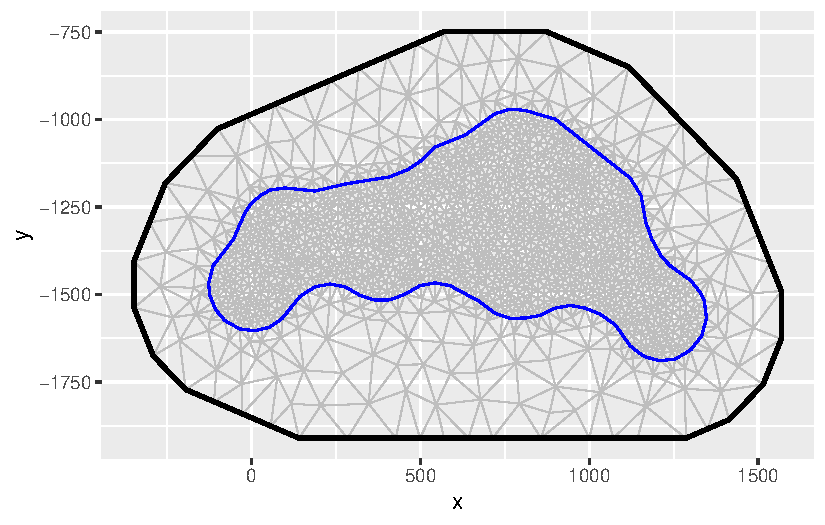
\includegraphics[keepaspectratio]{day5_practical_8_files/figure-pdf/unnamed-chunk-5-1.pdf}}

\subsection{domain boundary}

The \texttt{mexdolphin} object contains a predefined region of interest
which can be accessed through \texttt{mexdolphin\$ppoly}

\begin{Shaded}
\begin{Highlighting}[]
\NormalTok{mesh\_1 }\OtherTok{=} \FunctionTok{fm\_mesh\_2d}\NormalTok{(}\AttributeTok{boundary =}\NormalTok{ mexdolphin}\SpecialCharTok{$}\NormalTok{ppoly,}
                    \AttributeTok{max.edge =} \FunctionTok{c}\NormalTok{(}\DecValTok{30}\NormalTok{, }\DecValTok{150}\NormalTok{),}
                    \AttributeTok{cutoff =} \DecValTok{15}\NormalTok{,}
                    \AttributeTok{crs =} \FunctionTok{fm\_crs}\NormalTok{(mexdolphin}\SpecialCharTok{$}\NormalTok{points))}
\FunctionTok{ggplot}\NormalTok{() }\SpecialCharTok{+} \FunctionTok{gg}\NormalTok{(mesh\_1)}
\end{Highlighting}
\end{Shaded}

\pandocbounded{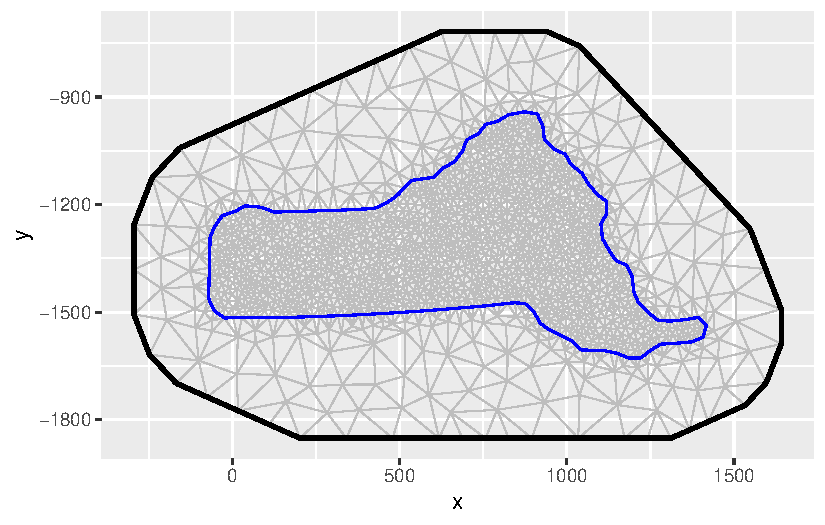
\includegraphics[keepaspectratio]{day5_practical_8_files/figure-pdf/unnamed-chunk-6-1.pdf}}

Key parameters in mesh construction include: \texttt{max.edge} for
maximum triangle edge lengths, \texttt{offset} for inner and outer
extensions (to prevent edge effects), and cutoff to avoid overly small
triangles in clustered areas.

\begin{tcolorbox}[enhanced jigsaw, colback=white, bottomrule=.15mm, arc=.35mm, opacitybacktitle=0.6, rightrule=.15mm, breakable, coltitle=black, toprule=.15mm, bottomtitle=1mm, toptitle=1mm, titlerule=0mm, left=2mm, leftrule=.75mm, title=\textcolor{quarto-callout-note-color}{\faInfo}\hspace{0.5em}{Note}, opacityback=0, colframe=quarto-callout-note-color-frame, colbacktitle=quarto-callout-note-color!10!white]

\textbf{General guidelines for creating the mesh}

\begin{enumerate}
\def\labelenumi{\arabic{enumi}.}
\tightlist
\item
  Create triangulation meshes with \texttt{fm\_mesh\_2d()}
\item
  Move undesired boundary effects away from the domain of interest by
  extending to a smooth external boundary
\item
  Use a coarser resolution in the extension to reduce computational cost
  (\texttt{max.edge=c(inner,\ outer)})
\item
  Use a fine resolution (subject to available computational resources)
  for the domain of interest (inner correlation range) and filter out
  small input point clusters (0 \textless{} \texttt{cutoff} \textless{}
  inner)
\item
  Coastlines and similar can be added to the domain specification in
  \texttt{fm\_mesh\_2d()} through the \texttt{boundary} argument.
\end{enumerate}

\end{tcolorbox}

\begin{tcolorbox}[enhanced jigsaw, colback=white, bottomrule=.15mm, arc=.35mm, opacitybacktitle=0.6, rightrule=.15mm, breakable, coltitle=black, toprule=.15mm, bottomtitle=1mm, toptitle=1mm, titlerule=0mm, left=2mm, leftrule=.75mm, title={Task}, opacityback=0, colframe=quarto-callout-warning-color-frame, colbacktitle=quarto-callout-warning-color!10!white]

Look at the documentation for the \texttt{fm\_mesh\_2d} function typing

\begin{Shaded}
\begin{Highlighting}[]
\NormalTok{?fm\_mesh\_2d}
\end{Highlighting}
\end{Shaded}

play around with the different options and create different meshes. You
can compare these against a pre-computed mesh available by typing
\texttt{plot(mexdolphin\$mesh)}

The \emph{rule of thumb} is that your mesh should be:

\begin{itemize}
\tightlist
\item
  fine enough to well represent the spatial variability of your process,
  but not too fine in order to avoid computation burden
\item
  the triangles should be regular, avoid long and thin triangles.
\item
  The mesh should contain a buffer around your area of interest (this is
  what is defined in the \texttt{offset} option) in order to avoid
  boundary artefact in the estimated variance.
\end{itemize}

\end{tcolorbox}

\subsubsection{Define the SPDE representation of the spatial
GF}\label{define-the-spde-representation-of-the-spatial-gf}

To define the SPDE representation of the spatial GF we use the function
\texttt{inla.spde2.pcmatern}. This takes as input the mesh we have
defined and the PC-priors definition for \(\rho\) and \(\sigma\) (the
range and the marginal standard deviation of the field).

PC priors Gaussian Random field are defined in (Fuglstad et al.~2018).
From a practical perspective for the range \(\rho\) you need to define
two paramters \(\rho_0\) and \(p_{\rho}\) such that you believe it is
reasonable that

\[
P(\rho<\rho_0)=p_{\rho}
\]

while for the marginal variance \(\sigma\) you need to define two
parameters \(\sigma_0\) and \(p_{\sigma}\) such that you believe it is
reasonable that

\[
P(\sigma>\sigma_0)=p_{\sigma}
\]

\begin{tcolorbox}[enhanced jigsaw, colback=white, bottomrule=.15mm, arc=.35mm, opacitybacktitle=0.6, rightrule=.15mm, breakable, coltitle=black, toprule=.15mm, bottomtitle=1mm, toptitle=1mm, titlerule=0mm, left=2mm, leftrule=.75mm, title={Question}, opacityback=0, colframe=quarto-callout-tip-color-frame, colbacktitle=quarto-callout-tip-color!10!white]

Take a look at the code below and select which of the following
statements about the specified Matern PC priors are true.

\begin{Shaded}
\begin{Highlighting}[]
\NormalTok{spde\_model }\OtherTok{\textless{}{-}} \FunctionTok{inla.spde2.pcmatern}\NormalTok{(mexdolphin}\SpecialCharTok{$}\NormalTok{mesh,}
  \AttributeTok{prior.sigma =} \FunctionTok{c}\NormalTok{(}\DecValTok{2}\NormalTok{, }\FloatTok{0.01}\NormalTok{),}
  \AttributeTok{prior.range =} \FunctionTok{c}\NormalTok{(}\DecValTok{50}\NormalTok{, }\FloatTok{0.01}\NormalTok{)}
\NormalTok{)}
\end{Highlighting}
\end{Shaded}

\begin{itemize}
\tightlist
\item
  \begin{enumerate}
  \def\labelenumi{(\Alph{enumi})}
  \tightlist
  \item
    there is probability of 0.01 that the spatial range is greater or
    equal than 50\\
  \end{enumerate}
\item
  \begin{enumerate}
  \def\labelenumi{(\Alph{enumi})}
  \setcounter{enumi}{1}
  \tightlist
  \item
    the probability that the spatial range is smaller than 50 is very
    small\\
  \end{enumerate}
\item
  \begin{enumerate}
  \def\labelenumi{(\Alph{enumi})}
  \setcounter{enumi}{2}
  \tightlist
  \item
    the probability that the marginal standard deviation is smaller than
    2 is very small\\
  \end{enumerate}
\item
  \begin{enumerate}
  \def\labelenumi{(\Alph{enumi})}
  \setcounter{enumi}{3}
  \tightlist
  \item
    there is probability of 0.99 that the marginal standard deviation is
    less or equal than 2
  \end{enumerate}
\end{itemize}

\end{tcolorbox}

\subsubsection{Define the components of the linear
predictor}\label{define-the-components-of-the-linear-predictor}

We have now defined a mesh and a SPDE representation of the spatial GF.
We now need to define the model components.

First, we need to define the detection function. Here, we will define a
half-normal detection probability function. This must take distance as
its first argument and the linear predictor of the sigma parameter as
its second:

\begin{Shaded}
\begin{Highlighting}[]
\NormalTok{hn }\OtherTok{\textless{}{-}} \ControlFlowTok{function}\NormalTok{(distance, sigma) \{}
  \FunctionTok{exp}\NormalTok{(}\SpecialCharTok{{-}}\FloatTok{0.5} \SpecialCharTok{*}\NormalTok{ (distance }\SpecialCharTok{/}\NormalTok{ sigma)}\SpecialCharTok{\^{}}\DecValTok{2}\NormalTok{)}
\NormalTok{\}}
\end{Highlighting}
\end{Shaded}

We need to now separately define the components of the model including
the SPDE model, the Intercept, the effect of depth and the detection
function parameter \texttt{sigma}.

\begin{Shaded}
\begin{Highlighting}[]
\NormalTok{cmp }\OtherTok{\textless{}{-}} \ErrorTok{\textasciitilde{}} \FunctionTok{space}\NormalTok{(}\AttributeTok{main =}\NormalTok{ geometry, }\AttributeTok{model =}\NormalTok{ spde\_model) }\SpecialCharTok{+}
  \FunctionTok{sigma}\NormalTok{(}\DecValTok{1}\NormalTok{,}
    \AttributeTok{prec.linear =} \DecValTok{1}\NormalTok{,}
    \AttributeTok{marginal =} \FunctionTok{bm\_marginal}\NormalTok{(qexp, pexp, dexp, }\AttributeTok{rate =} \DecValTok{1} \SpecialCharTok{/} \DecValTok{8}\NormalTok{)}
\NormalTok{  ) }\SpecialCharTok{+}
  \FunctionTok{Intercept}\NormalTok{(}\DecValTok{1}\NormalTok{)}
\end{Highlighting}
\end{Shaded}

\begin{tcolorbox}[enhanced jigsaw, colback=white, bottomrule=.15mm, arc=.35mm, opacitybacktitle=0.6, rightrule=.15mm, breakable, coltitle=black, toprule=.15mm, bottomtitle=1mm, toptitle=1mm, titlerule=0mm, left=2mm, leftrule=.75mm, title=\textcolor{quarto-callout-note-color}{\faInfo}\hspace{0.5em}{Note}, opacityback=0, colframe=quarto-callout-note-color-frame, colbacktitle=quarto-callout-note-color!10!white]

To control the prior distribution for the \texttt{sigma} parameter, we
use a transformation mapper that converts a latent variable into an
exponentially distributed variable with expectation 8 (this is a
somewhat arbitrary value, but motivated by the maximum observation
distance W)

The \texttt{marginal} argument in the \texttt{sigma} component specifies
the transformation function taking N(0,1) to Exponential(1/8).

\end{tcolorbox}

The formula, which describes how these components are combined to form
the linear predictor

\[\log \color{red}{\tilde{\lambda}(s)} = \overbrace{\log \lambda (s)}^{\beta_0 + \xi(s)} + \overbrace{\log \color{red}{g(d(s))}}^{-0.5~d(\mathbf{s})^2\sigma^{-2}}\]

\begin{Shaded}
\begin{Highlighting}[]
\NormalTok{eta }\OtherTok{\textless{}{-}}\NormalTok{ geometry }\SpecialCharTok{+}\NormalTok{ distance }\SpecialCharTok{\textasciitilde{}}\NormalTok{ space }\SpecialCharTok{+}
  \FunctionTok{log}\NormalTok{(}\FunctionTok{hn}\NormalTok{(distance, sigma)) }\SpecialCharTok{+}
\NormalTok{  Intercept }\SpecialCharTok{+} \FunctionTok{log}\NormalTok{(}\DecValTok{2}\NormalTok{) }
\end{Highlighting}
\end{Shaded}

Here, the \texttt{log(2)} offset in the predictor takes care of the
two-sided detections

\subsubsection{Define the observation
model}\label{define-the-observation-model}

\texttt{inlabru} has support for latent Gaussian Cox processes through
the \texttt{cp} likelihood family. To fit a point process model recall
that we need to approximate the integral in using a numerical
integration scheme as:

\[
\approx\exp\left(-\sum_{k=1}^{N_k}w_k\lambda(s_k)\right)\prod_{i=1}^n \lambda(\mathbf{s}_i)
\]

Thus, we first create our integration scheme using the \texttt{fm\_int}
function by specifying integration domains for the spatial and distance
dimensions.

Here we use the same points to define the SPDE approximation and to
approximate the integral in Equation~\ref{eq-thinned_pp}, so that the
integration weight and SPDE weights are consistent with each other. We
also need to explicitly integrate over the distance dimension so we use
the \texttt{fm\_mesh\_1d()} to create mesh over the samplers (which are
the transect lines in this dataset, so we need to tell \texttt{inlabru}
about the strip half-width).

\begin{Shaded}
\begin{Highlighting}[]
\CommentTok{\# build integration scheme}
\NormalTok{distance\_domain }\OtherTok{\textless{}{-}}  \FunctionTok{fm\_mesh\_1d}\NormalTok{(}\FunctionTok{seq}\NormalTok{(}\DecValTok{0}\NormalTok{, }\DecValTok{8}\NormalTok{,}
                              \AttributeTok{length.out =} \DecValTok{30}\NormalTok{))}
\NormalTok{ips }\OtherTok{=} \FunctionTok{fm\_int}\NormalTok{(}\FunctionTok{list}\NormalTok{(}\AttributeTok{geometry =}\NormalTok{ mexdolphin}\SpecialCharTok{$}\NormalTok{mesh,}
                  \AttributeTok{distance =}\NormalTok{ distance\_domain),}
             \AttributeTok{samplers =}\NormalTok{ mexdolphin}\SpecialCharTok{$}\NormalTok{samplers)}
\end{Highlighting}
\end{Shaded}

Now, we just need to supply the \texttt{sf} object as our data and the
integration scheme \texttt{ips}:

\begin{Shaded}
\begin{Highlighting}[]
\NormalTok{lik }\OtherTok{=} \FunctionTok{bru\_obs}\NormalTok{(}\StringTok{"cp"}\NormalTok{,}
              \AttributeTok{formula =}\NormalTok{ eta,}
              \AttributeTok{data =}\NormalTok{ mexdolphin}\SpecialCharTok{$}\NormalTok{points,}
              \AttributeTok{ips =}\NormalTok{ ips)}
\end{Highlighting}
\end{Shaded}

Then we fit the model, passing both the components and the observaional
model

\begin{Shaded}
\begin{Highlighting}[]
\NormalTok{fit }\OtherTok{=} \FunctionTok{bru}\NormalTok{(cmp, lik)}
\end{Highlighting}
\end{Shaded}

\begin{tcolorbox}[enhanced jigsaw, colback=white, bottomrule=.15mm, arc=.35mm, opacitybacktitle=0.6, rightrule=.15mm, breakable, coltitle=black, toprule=.15mm, bottomtitle=1mm, toptitle=1mm, titlerule=0mm, left=2mm, leftrule=.75mm, title=\textcolor{quarto-callout-note-color}{\faInfo}\hspace{0.5em}{Note}, opacityback=0, colframe=quarto-callout-note-color-frame, colbacktitle=quarto-callout-note-color!10!white]

\texttt{inlabru} supports a shortcut for defining the integration points
using the \texttt{domain} and \texttt{samplers} argument of
\texttt{bru\_obs()}. This \texttt{domain} argument expects a list of
named domains with inputs that are then internally passed to
\texttt{fm\_int()} to build the integration scheme. The
\texttt{samplers} argument is used to define subsets of the domain over
which the integral should be computed. An equivalent way to define the
same model as above is:

\begin{Shaded}
\begin{Highlighting}[]
\NormalTok{lik }\OtherTok{=} \FunctionTok{bru\_obs}\NormalTok{(}\AttributeTok{formula =}\NormalTok{ eta, }
              \AttributeTok{data =}\NormalTok{ mexdolphin}\SpecialCharTok{$}\NormalTok{points, }
              \AttributeTok{family =} \StringTok{"cp"}\NormalTok{,}
              \AttributeTok{domain =} \FunctionTok{list}\NormalTok{(}
                \AttributeTok{geometry =}\NormalTok{ mesh,}
                \AttributeTok{distance =} \FunctionTok{fm\_mesh\_1d}\NormalTok{(}\FunctionTok{seq}\NormalTok{(}\DecValTok{0}\NormalTok{, }\DecValTok{8}\NormalTok{, }\AttributeTok{length.out =} \DecValTok{30}\NormalTok{))),}
              \AttributeTok{samplers =}\NormalTok{ mexdolphin}\SpecialCharTok{$}\NormalTok{samplers)}
\end{Highlighting}
\end{Shaded}

\end{tcolorbox}

\subsection{Visualize model Results}\label{visualize-model-results}

\subsubsection{Posterior summaries}\label{posterior-summaries}

We can use the \texttt{fit\$summary.fixed} and \texttt{summary.hyperpar}
to obtain posterior summaries of the model parameters.

\begin{table}
\fontsize{12.0pt}{14.0pt}\selectfont
\begin{tabular*}{\linewidth}{@{\extracolsep{\fill}}l|rrr}
\toprule
 & mean & 0.025quant & 0.975quant \\ 
\midrule\addlinespace[2.5pt]
sigma & -0.05 & -0.46 & 0.36 \\ 
Intercept & -8.16 & -9.29 & -7.34 \\ 
Range for space & 295.48 & 110.54 & 673.68 \\ 
Stdev for space & 0.81 & 0.42 & 1.39 \\ 
\bottomrule
\end{tabular*}
\end{table}

Look at the SPDE parameter posteriors as follows:

\begin{Shaded}
\begin{Highlighting}[]
\FunctionTok{plot}\NormalTok{( }\FunctionTok{spde.posterior}\NormalTok{(fit, }\StringTok{"space"}\NormalTok{, }\AttributeTok{what =} \StringTok{"range"}\NormalTok{)) }\SpecialCharTok{+}
\FunctionTok{plot}\NormalTok{( }\FunctionTok{spde.posterior}\NormalTok{(fit, }\StringTok{"space"}\NormalTok{, }\AttributeTok{what =} \StringTok{"log.variance"}\NormalTok{))  }
\end{Highlighting}
\end{Shaded}

\pandocbounded{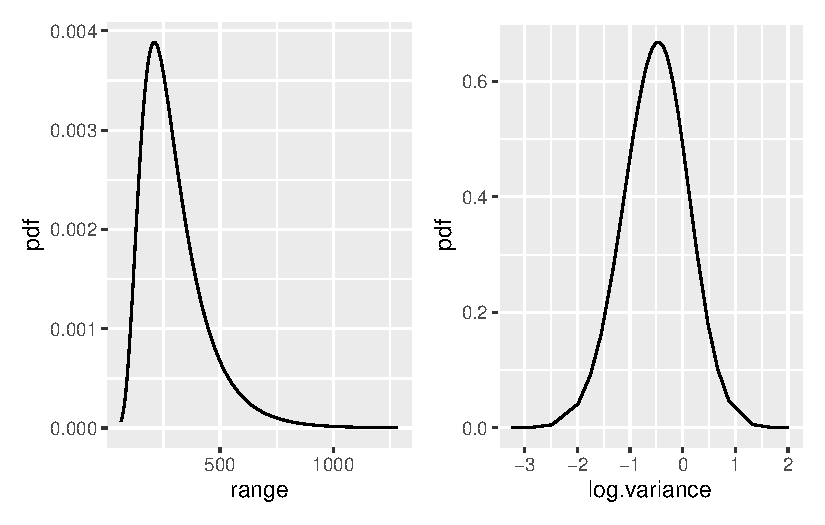
\includegraphics[keepaspectratio]{day5_practical_8_files/figure-pdf/unnamed-chunk-18-1.pdf}}

\subsubsection{Model predictions}\label{model-predictions}

We now want to extract the estimated posterior mean and sd of spatial
GF. To do this we first need to define a grid of points where we want to
predict. We do this using the function \texttt{fm\_pixel()} which
creates a regular grid of points covering the mesh

\begin{Shaded}
\begin{Highlighting}[]
\NormalTok{pxl }\OtherTok{\textless{}{-}} \FunctionTok{fm\_pixels}\NormalTok{(mexdolphin}\SpecialCharTok{$}\NormalTok{mesh, }\AttributeTok{dims =} \FunctionTok{c}\NormalTok{(}\DecValTok{200}\NormalTok{, }\DecValTok{100}\NormalTok{), }\AttributeTok{mask =}\NormalTok{ mexdolphin}\SpecialCharTok{$}\NormalTok{ppoly)}
\end{Highlighting}
\end{Shaded}

then compute the prediction for both the spatial GF and the linear
predictor (spatial GF + intercept)

\begin{Shaded}
\begin{Highlighting}[]
\NormalTok{pr.int }\OtherTok{=} \FunctionTok{predict}\NormalTok{(fit, pxl, }\SpecialCharTok{\textasciitilde{}}\FunctionTok{data.frame}\NormalTok{(}\AttributeTok{spatial =}\NormalTok{ space,}
                                      \AttributeTok{lambda =} \FunctionTok{exp}\NormalTok{(Intercept }\SpecialCharTok{+}\NormalTok{ space)))}
\end{Highlighting}
\end{Shaded}

Finally, we can plot the maps of the spatial effect

\begin{Shaded}
\begin{Highlighting}[]
\FunctionTok{ggplot}\NormalTok{() }\SpecialCharTok{+} \FunctionTok{geom\_sf}\NormalTok{(}\AttributeTok{data =}\NormalTok{ pr.int}\SpecialCharTok{$}\NormalTok{spatial,}\FunctionTok{aes}\NormalTok{(}\AttributeTok{color =}\NormalTok{ mean)) }\SpecialCharTok{+} \FunctionTok{scale\_color\_scico}\NormalTok{() }\SpecialCharTok{+} \FunctionTok{ggtitle}\NormalTok{(}\StringTok{"Posterior mean"}\NormalTok{)}
\end{Highlighting}
\end{Shaded}

\pandocbounded{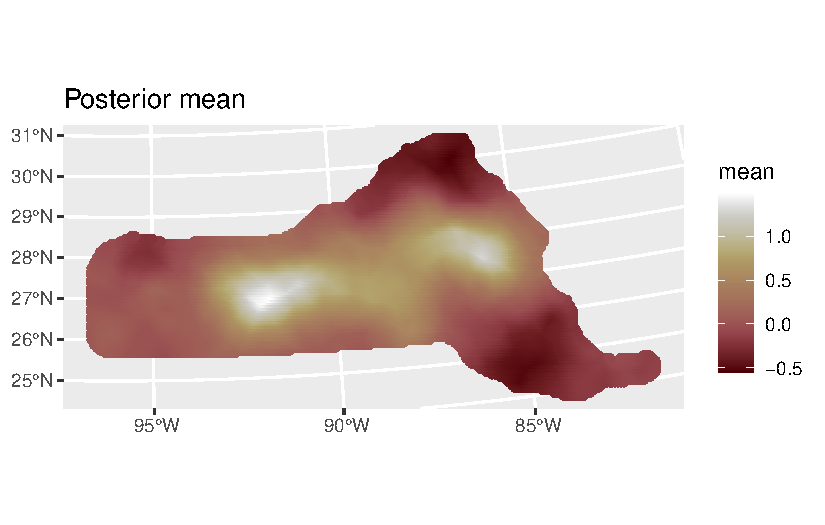
\includegraphics[keepaspectratio]{day5_practical_8_files/figure-pdf/unnamed-chunk-21-1.pdf}}

\begin{Shaded}
\begin{Highlighting}[]
\FunctionTok{ggplot}\NormalTok{() }\SpecialCharTok{+} \FunctionTok{geom\_sf}\NormalTok{(}\AttributeTok{data =}\NormalTok{ pr.int}\SpecialCharTok{$}\NormalTok{spatial,}\FunctionTok{aes}\NormalTok{(}\AttributeTok{color =}\NormalTok{ sd)) }\SpecialCharTok{+} \FunctionTok{scale\_color\_scico}\NormalTok{() }\SpecialCharTok{+} \FunctionTok{ggtitle}\NormalTok{(}\StringTok{"Posterior sd"}\NormalTok{)}
\end{Highlighting}
\end{Shaded}

\pandocbounded{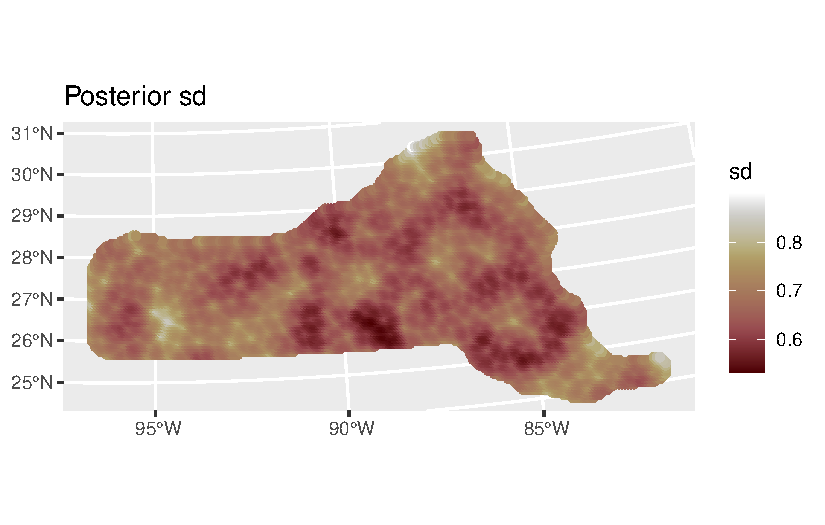
\includegraphics[keepaspectratio]{day5_practical_8_files/figure-pdf/unnamed-chunk-21-2.pdf}}

\textbf{Note} The posterior sd is lowest at the observation points. Note
how the posterior sd is inflated around the border, this is the ``border
effect'' due to the SPDE representation.

\begin{tcolorbox}[enhanced jigsaw, colback=white, bottomrule=.15mm, arc=.35mm, opacitybacktitle=0.6, rightrule=.15mm, breakable, coltitle=black, toprule=.15mm, bottomtitle=1mm, toptitle=1mm, titlerule=0mm, left=2mm, leftrule=.75mm, title={Task}, opacityback=0, colframe=quarto-callout-warning-color-frame, colbacktitle=quarto-callout-warning-color!10!white]

Using the predictions stored in \texttt{pr.int}, produce a map of the
posterior mean intensity.

Take hint

Recall that the predicted intensity is given by
\(\lambda(s) = \exp(\beta_0+\xi(s))\)

Click here to see the solution

\begin{Shaded}
\begin{Highlighting}[]
\FunctionTok{ggplot}\NormalTok{() }\SpecialCharTok{+} 
  \FunctionTok{geom\_sf}\NormalTok{(}\AttributeTok{data =}\NormalTok{ pr.int}\SpecialCharTok{$}\NormalTok{lambda,}\FunctionTok{aes}\NormalTok{(}\AttributeTok{color =}\NormalTok{ mean)) }\SpecialCharTok{+}
  \FunctionTok{scale\_color\_scico}\NormalTok{(}\AttributeTok{palette =} \StringTok{"imola"}\NormalTok{) }\SpecialCharTok{+}
  \FunctionTok{ggtitle}\NormalTok{(}\StringTok{"Posterior mean"}\NormalTok{)}
\end{Highlighting}
\end{Shaded}

\begin{center}
\pandocbounded{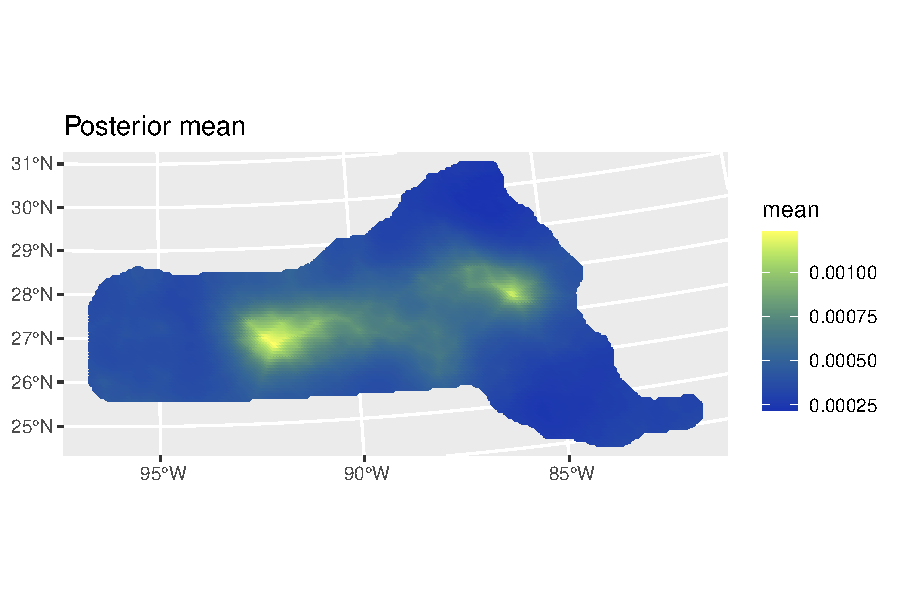
\includegraphics[keepaspectratio]{day5_practical_8_files/figure-pdf/unnamed-chunk-22-1.pdf}}
\end{center}

\end{tcolorbox}

We can predict the detection function in a similar fashion.Here, we
should make sure that it doesn't try to evaluate the effects of
components that can't be evaluated using the given input data.

\begin{Shaded}
\begin{Highlighting}[]
\NormalTok{distdf }\OtherTok{\textless{}{-}} \FunctionTok{data.frame}\NormalTok{(}\AttributeTok{distance =} \FunctionTok{seq}\NormalTok{(}\DecValTok{0}\NormalTok{, }\DecValTok{8}\NormalTok{, }\AttributeTok{length.out =} \DecValTok{100}\NormalTok{))}
\NormalTok{dfun }\OtherTok{\textless{}{-}} \FunctionTok{predict}\NormalTok{(fit, distdf, }\SpecialCharTok{\textasciitilde{}} \FunctionTok{hn}\NormalTok{(distance, sigma))}
\FunctionTok{plot}\NormalTok{(dfun)}
\end{Highlighting}
\end{Shaded}

\pandocbounded{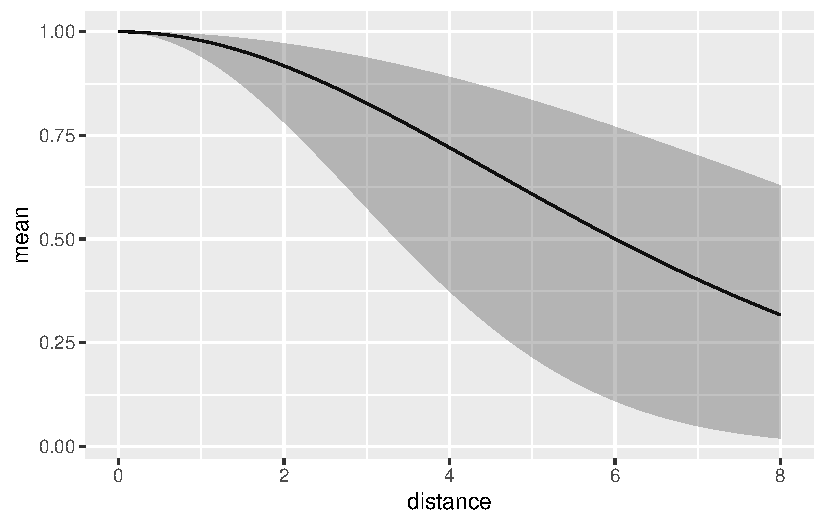
\includegraphics[keepaspectratio]{day5_practical_8_files/figure-pdf/unnamed-chunk-23-1.pdf}}

\subsection{Abundance estimates}\label{abundance-estimates}

The mean expected number of animals can be computed by integrating the
intensity over the region of interest as follows:

\begin{Shaded}
\begin{Highlighting}[]
\NormalTok{predpts }\OtherTok{\textless{}{-}} \FunctionTok{fm\_int}\NormalTok{(mexdolphin}\SpecialCharTok{$}\NormalTok{mesh, mexdolphin}\SpecialCharTok{$}\NormalTok{ppoly)}
\NormalTok{Lambda }\OtherTok{\textless{}{-}} \FunctionTok{predict}\NormalTok{(fit, predpts, }\SpecialCharTok{\textasciitilde{}} \FunctionTok{sum}\NormalTok{(weight }\SpecialCharTok{*} \FunctionTok{exp}\NormalTok{(space }\SpecialCharTok{+}\NormalTok{ Intercept)))}
\NormalTok{Lambda}
\end{Highlighting}
\end{Shaded}

\begin{verbatim}
      mean       sd   q0.025     q0.5   q0.975   median sd.mc_std_err
1 245.8929 49.52867 164.5492 246.5204 351.8935 246.5204      3.726218
  mean.mc_std_err
1        5.698111
\end{verbatim}

To fully propagate the uncertainty on the expected number animals we can
draw Monte Carlo samples from the fitted model as follows (this could
take a couple of minutes):

\begin{Shaded}
\begin{Highlighting}[]
\NormalTok{Ns }\OtherTok{\textless{}{-}} \FunctionTok{seq}\NormalTok{(}\DecValTok{50}\NormalTok{, }\DecValTok{450}\NormalTok{, }\AttributeTok{by =} \DecValTok{1}\NormalTok{)}
\NormalTok{Nest }\OtherTok{\textless{}{-}} \FunctionTok{predict}\NormalTok{(fit, predpts,}
  \SpecialCharTok{\textasciitilde{}} \FunctionTok{data.frame}\NormalTok{(}
    \AttributeTok{N =}\NormalTok{ Ns,}
    \AttributeTok{density =} \FunctionTok{dpois}\NormalTok{(}
\NormalTok{      Ns,}
      \AttributeTok{lambda =} \FunctionTok{sum}\NormalTok{(weight }\SpecialCharTok{*} \FunctionTok{exp}\NormalTok{(space }\SpecialCharTok{+}\NormalTok{ Intercept))}
\NormalTok{    )}
\NormalTok{  ),}
  \AttributeTok{n.samples =} \DecValTok{2000}
\NormalTok{)}
\end{Highlighting}
\end{Shaded}

We can compare this with a simpler ``plug-in'' approximation:

\begin{Shaded}
\begin{Highlighting}[]
\NormalTok{Nest }\OtherTok{\textless{}{-}}\NormalTok{ dplyr}\SpecialCharTok{::}\FunctionTok{bind\_rows}\NormalTok{(}
  \FunctionTok{cbind}\NormalTok{(Nest, }\AttributeTok{Method =} \StringTok{"Posterior"}\NormalTok{),}
  \FunctionTok{data.frame}\NormalTok{(}
    \AttributeTok{N =}\NormalTok{ Nest}\SpecialCharTok{$}\NormalTok{N,}
    \AttributeTok{mean =} \FunctionTok{dpois}\NormalTok{(Nest}\SpecialCharTok{$}\NormalTok{N, }\AttributeTok{lambda =}\NormalTok{ Lambda}\SpecialCharTok{$}\NormalTok{mean),}
    \AttributeTok{mean.mc\_std\_err =} \DecValTok{0}\NormalTok{,}
    \AttributeTok{Method =} \StringTok{"Plugin"}
\NormalTok{  )}
\NormalTok{)}
\end{Highlighting}
\end{Shaded}

Then, we can visualize the result as follows:

\begin{Shaded}
\begin{Highlighting}[]
\FunctionTok{ggplot}\NormalTok{(}\AttributeTok{data =}\NormalTok{ Nest) }\SpecialCharTok{+}
  \FunctionTok{geom\_line}\NormalTok{(}\FunctionTok{aes}\NormalTok{(}\AttributeTok{x =}\NormalTok{ N, }\AttributeTok{y =}\NormalTok{ mean, }\AttributeTok{colour =}\NormalTok{ Method)) }\SpecialCharTok{+}
  \FunctionTok{geom\_ribbon}\NormalTok{(}
    \FunctionTok{aes}\NormalTok{(}
      \AttributeTok{x =}\NormalTok{ N,}
      \AttributeTok{ymin =}\NormalTok{ mean }\SpecialCharTok{{-}} \DecValTok{2} \SpecialCharTok{*}\NormalTok{ mean.mc\_std\_err,}
      \AttributeTok{ymax =}\NormalTok{ mean }\SpecialCharTok{+} \DecValTok{2} \SpecialCharTok{*}\NormalTok{ mean.mc\_std\_err,}
      \AttributeTok{fill =}\NormalTok{ Method,}
\NormalTok{    ),}
    \AttributeTok{alpha =} \FloatTok{0.2}
\NormalTok{  ) }\SpecialCharTok{+}
  \FunctionTok{geom\_line}\NormalTok{(}\FunctionTok{aes}\NormalTok{(}\AttributeTok{x =}\NormalTok{ N, }\AttributeTok{y =}\NormalTok{ mean, }\AttributeTok{colour =}\NormalTok{ Method)) }\SpecialCharTok{+}
  \FunctionTok{ylab}\NormalTok{(}\StringTok{"Probability mass function"}\NormalTok{)}
\end{Highlighting}
\end{Shaded}

\pandocbounded{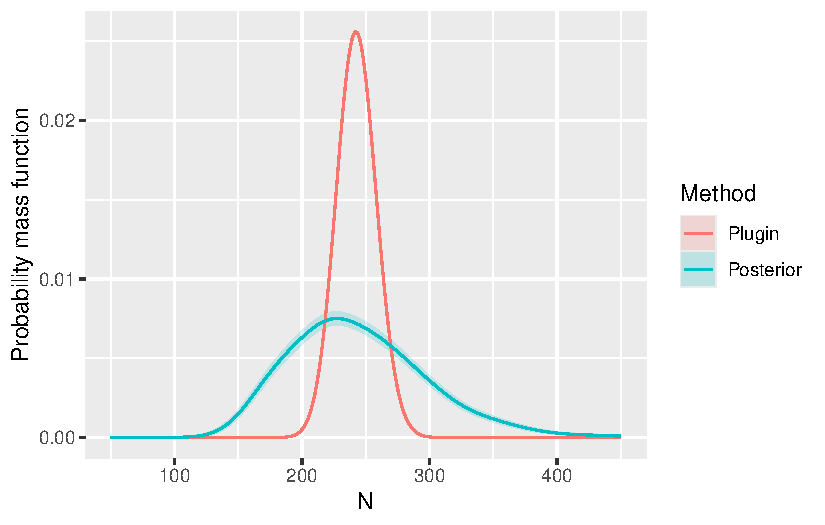
\includegraphics[keepaspectratio]{day5_practical_8_files/figure-pdf/unnamed-chunk-27-1.pdf}}

\subsection{Model checks}\label{model-checks}

Lastly, we can assess the goodness-of-fit of the models by comparing the
observed counts across different distance bins and the expected counts
and their associated uncertainty:

\begin{Shaded}
\begin{Highlighting}[]
\NormalTok{bc }\OtherTok{\textless{}{-}} \FunctionTok{bincount}\NormalTok{(}
  \AttributeTok{result =}\NormalTok{ fit,}
  \AttributeTok{observations =}\NormalTok{ mexdolphin}\SpecialCharTok{$}\NormalTok{points}\SpecialCharTok{$}\NormalTok{distance,}
  \AttributeTok{breaks =} \FunctionTok{seq}\NormalTok{(}\DecValTok{0}\NormalTok{, }\FunctionTok{max}\NormalTok{(mexdolphin}\SpecialCharTok{$}\NormalTok{points}\SpecialCharTok{$}\NormalTok{distance), }\AttributeTok{length.out =} \DecValTok{9}\NormalTok{),}
  \AttributeTok{predictor =}\NormalTok{ distance }\SpecialCharTok{\textasciitilde{}} \FunctionTok{hn}\NormalTok{(distance, sigma)}
\NormalTok{)}
\FunctionTok{attributes}\NormalTok{(bc)}\SpecialCharTok{$}\NormalTok{ggp}
\end{Highlighting}
\end{Shaded}

\pandocbounded{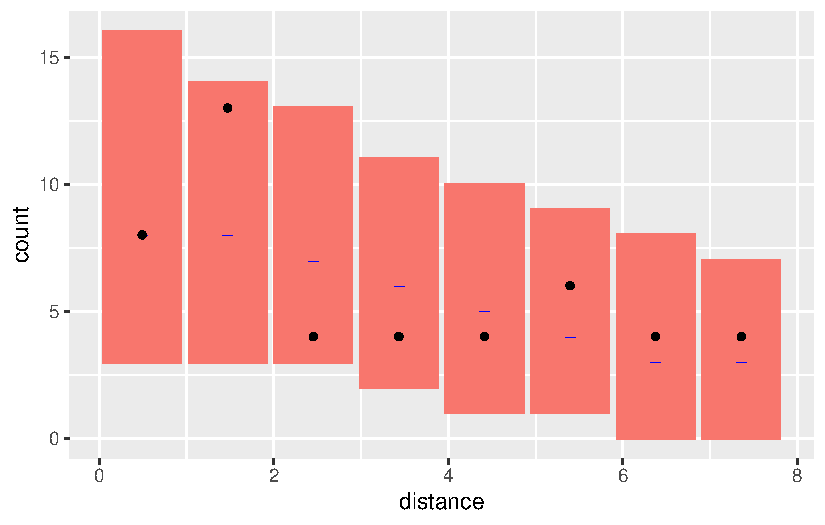
\includegraphics[keepaspectratio]{day5_practical_8_files/figure-pdf/unnamed-chunk-28-1.pdf}}

\begin{tcolorbox}[enhanced jigsaw, colback=white, bottomrule=.15mm, arc=.35mm, opacitybacktitle=0.6, rightrule=.15mm, breakable, coltitle=black, toprule=.15mm, bottomtitle=1mm, toptitle=1mm, titlerule=0mm, left=2mm, leftrule=.75mm, title={Task}, opacityback=0, colframe=quarto-callout-warning-color-frame, colbacktitle=quarto-callout-warning-color!10!white]

Fit a model using a hazard detection function instead and compare the
GoF of this model with that from the half-normal detection model. Recall
that the hazard detection function is given by:

\[
g(\mathbf{s}|\sigma) = 1 - \exp(-(d(\mathbf{s})/\sigma)^{-1})
\]

Take hint

The hazard function can be codes as:

\begin{Shaded}
\begin{Highlighting}[]
\NormalTok{hr }\OtherTok{\textless{}{-}} \ControlFlowTok{function}\NormalTok{(distance, sigma) \{}
  \DecValTok{1} \SpecialCharTok{{-}} \FunctionTok{exp}\NormalTok{(}\SpecialCharTok{{-}}\NormalTok{(distance }\SpecialCharTok{/}\NormalTok{ sigma)}\SpecialCharTok{\^{}{-}}\DecValTok{1}\NormalTok{)}
\NormalTok{\}}
\end{Highlighting}
\end{Shaded}

You can use the same prior for the \texttt{sigma} parameter as for the
half-Normal model (such parameters aren't always comparable, but in this
example it's a reasonable choice). You can also use the \texttt{lgcp}
function as a shortcut to fit the model (type \texttt{?lgcp} for further
details).

Click here to see the solution

\begin{Shaded}
\begin{Highlighting}[]
\NormalTok{formula1 }\OtherTok{\textless{}{-}}\NormalTok{ geometry }\SpecialCharTok{+}\NormalTok{ distance }\SpecialCharTok{\textasciitilde{}}\NormalTok{ space }\SpecialCharTok{+}
  \FunctionTok{log}\NormalTok{(}\FunctionTok{hr}\NormalTok{(distance, sigma)) }\SpecialCharTok{+}
\NormalTok{  Intercept }\SpecialCharTok{+} \FunctionTok{log}\NormalTok{(}\DecValTok{2}\NormalTok{)}

\CommentTok{\# here we use the shorcut to specify the model}
\NormalTok{fit1 }\OtherTok{\textless{}{-}} \FunctionTok{lgcp}\NormalTok{(}
  \AttributeTok{components =}\NormalTok{ cmp,}
\NormalTok{  mexdolphin}\SpecialCharTok{$}\NormalTok{points,}
  \AttributeTok{samplers =}\NormalTok{ mexdolphin}\SpecialCharTok{$}\NormalTok{samplers,}
  \AttributeTok{domain =} \FunctionTok{list}\NormalTok{(}
    \AttributeTok{geometry =}\NormalTok{ mexdolphin}\SpecialCharTok{$}\NormalTok{mesh,}
    \AttributeTok{distance =} \FunctionTok{fm\_mesh\_1d}\NormalTok{(}\FunctionTok{seq}\NormalTok{(}\DecValTok{0}\NormalTok{, }\DecValTok{8}\NormalTok{, }\AttributeTok{length.out =} \DecValTok{30}\NormalTok{))}
\NormalTok{  ),}
  \AttributeTok{formula =}\NormalTok{ formula1}
\NormalTok{)}

\NormalTok{bc1 }\OtherTok{\textless{}{-}} \FunctionTok{bincount}\NormalTok{(}
  \AttributeTok{result =}\NormalTok{ fit1,}
  \AttributeTok{observations =}\NormalTok{ mexdolphin}\SpecialCharTok{$}\NormalTok{points}\SpecialCharTok{$}\NormalTok{distance,}
  \AttributeTok{breaks =} \FunctionTok{seq}\NormalTok{(}\DecValTok{0}\NormalTok{, }\FunctionTok{max}\NormalTok{(mexdolphin}\SpecialCharTok{$}\NormalTok{points}\SpecialCharTok{$}\NormalTok{distance), }\AttributeTok{length.out =} \DecValTok{9}\NormalTok{),}
  \AttributeTok{predictor =}\NormalTok{ distance }\SpecialCharTok{\textasciitilde{}} \FunctionTok{hn}\NormalTok{(distance, sigma)}
\NormalTok{)}
\FunctionTok{attributes}\NormalTok{(bc1)}\SpecialCharTok{$}\NormalTok{ggp}
\end{Highlighting}
\end{Shaded}

\begin{center}
\pandocbounded{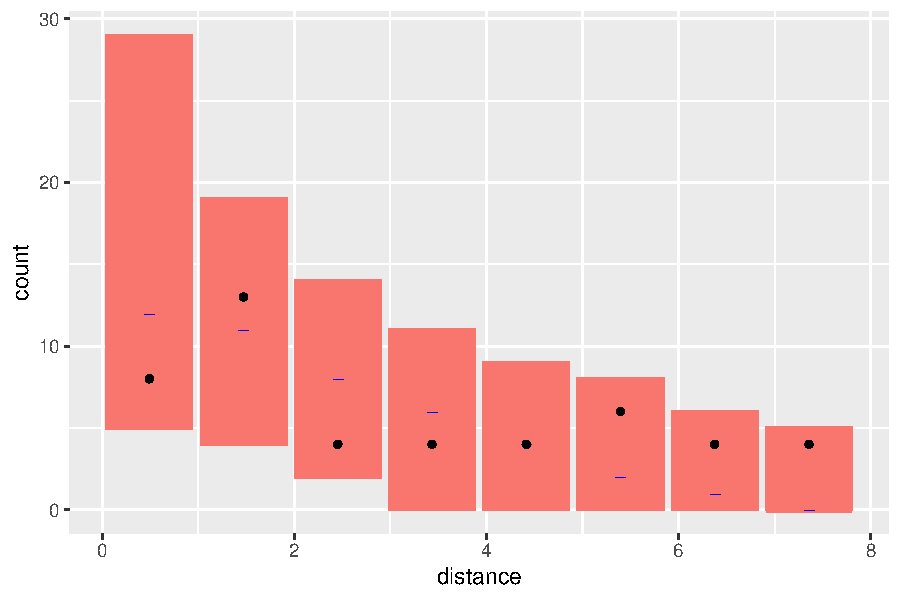
\includegraphics[keepaspectratio]{day5_practical_8_files/figure-pdf/unnamed-chunk-30-1.pdf}}
\end{center}

\end{tcolorbox}

\begin{Shaded}
\begin{Highlighting}[]
\FunctionTok{library}\NormalTok{(dplyr)}
\FunctionTok{library}\NormalTok{(ggplot2)}
\FunctionTok{library}\NormalTok{(inlabru)}
\FunctionTok{library}\NormalTok{(INLA)}
\FunctionTok{library}\NormalTok{(terra)}
\FunctionTok{library}\NormalTok{(sf)}
\FunctionTok{library}\NormalTok{(scico)}
\FunctionTok{library}\NormalTok{(magrittr)}
\FunctionTok{library}\NormalTok{(patchwork)}
\FunctionTok{library}\NormalTok{(tidyterra)}


\CommentTok{\# We want to obtain CPO data from the estimations}
\FunctionTok{bru\_options\_set}\NormalTok{(}\AttributeTok{control.compute =} \FunctionTok{list}\NormalTok{(}\AttributeTok{dic =} \ConstantTok{TRUE}\NormalTok{,}
                                       \AttributeTok{waic =} \ConstantTok{TRUE}\NormalTok{,}
                                       \AttributeTok{mlik =} \ConstantTok{TRUE}\NormalTok{,}
                                       \AttributeTok{cpo =} \ConstantTok{TRUE}\NormalTok{))}
\end{Highlighting}
\end{Shaded}

In this practical we are going to work with data with excess zeros. We
will

\begin{itemize}
\item
  \hyperref[sec-prep]{Create count data from a \texttt{gorillas}
  dataset}
\item
  Fit a \hyperref[sec-zip]{zero inflated model}
\item
  Fit a \hyperref[sec-zap]{hurdle model}
\item
  Fit a \hyperref[sec-two-lik]{hurdle model using two likelihoods}
\item
  Fit a \hyperref[sec-two-lik-share]{hurdle model using two likelihoods
  and a shared component}
\end{itemize}

\section{Data Preparation}\label{sec-prep}

The following example use the \texttt{gorillas} dataset available in the
\texttt{inlabru} library.

The data give the locations of Gorilla's nests in an area: ::: \{.cell
layout-align=``center''\}

\begin{Shaded}
\begin{Highlighting}[]
\NormalTok{gorillas\_sf }\OtherTok{\textless{}{-}}\NormalTok{ inlabru}\SpecialCharTok{::}\NormalTok{gorillas\_sf}
\NormalTok{nests }\OtherTok{\textless{}{-}}\NormalTok{ gorillas\_sf}\SpecialCharTok{$}\NormalTok{nests}
\NormalTok{boundary }\OtherTok{\textless{}{-}}\NormalTok{ gorillas\_sf}\SpecialCharTok{$}\NormalTok{boundary}

\FunctionTok{ggplot}\NormalTok{() }\SpecialCharTok{+} \FunctionTok{geom\_sf}\NormalTok{(}\AttributeTok{data =}\NormalTok{ nests) }\SpecialCharTok{+}
  \FunctionTok{geom\_sf}\NormalTok{(}\AttributeTok{data =}\NormalTok{ boundary, }\AttributeTok{alpha =} \DecValTok{0}\NormalTok{)}
\end{Highlighting}
\end{Shaded}

\begin{figure}[H]

{\centering 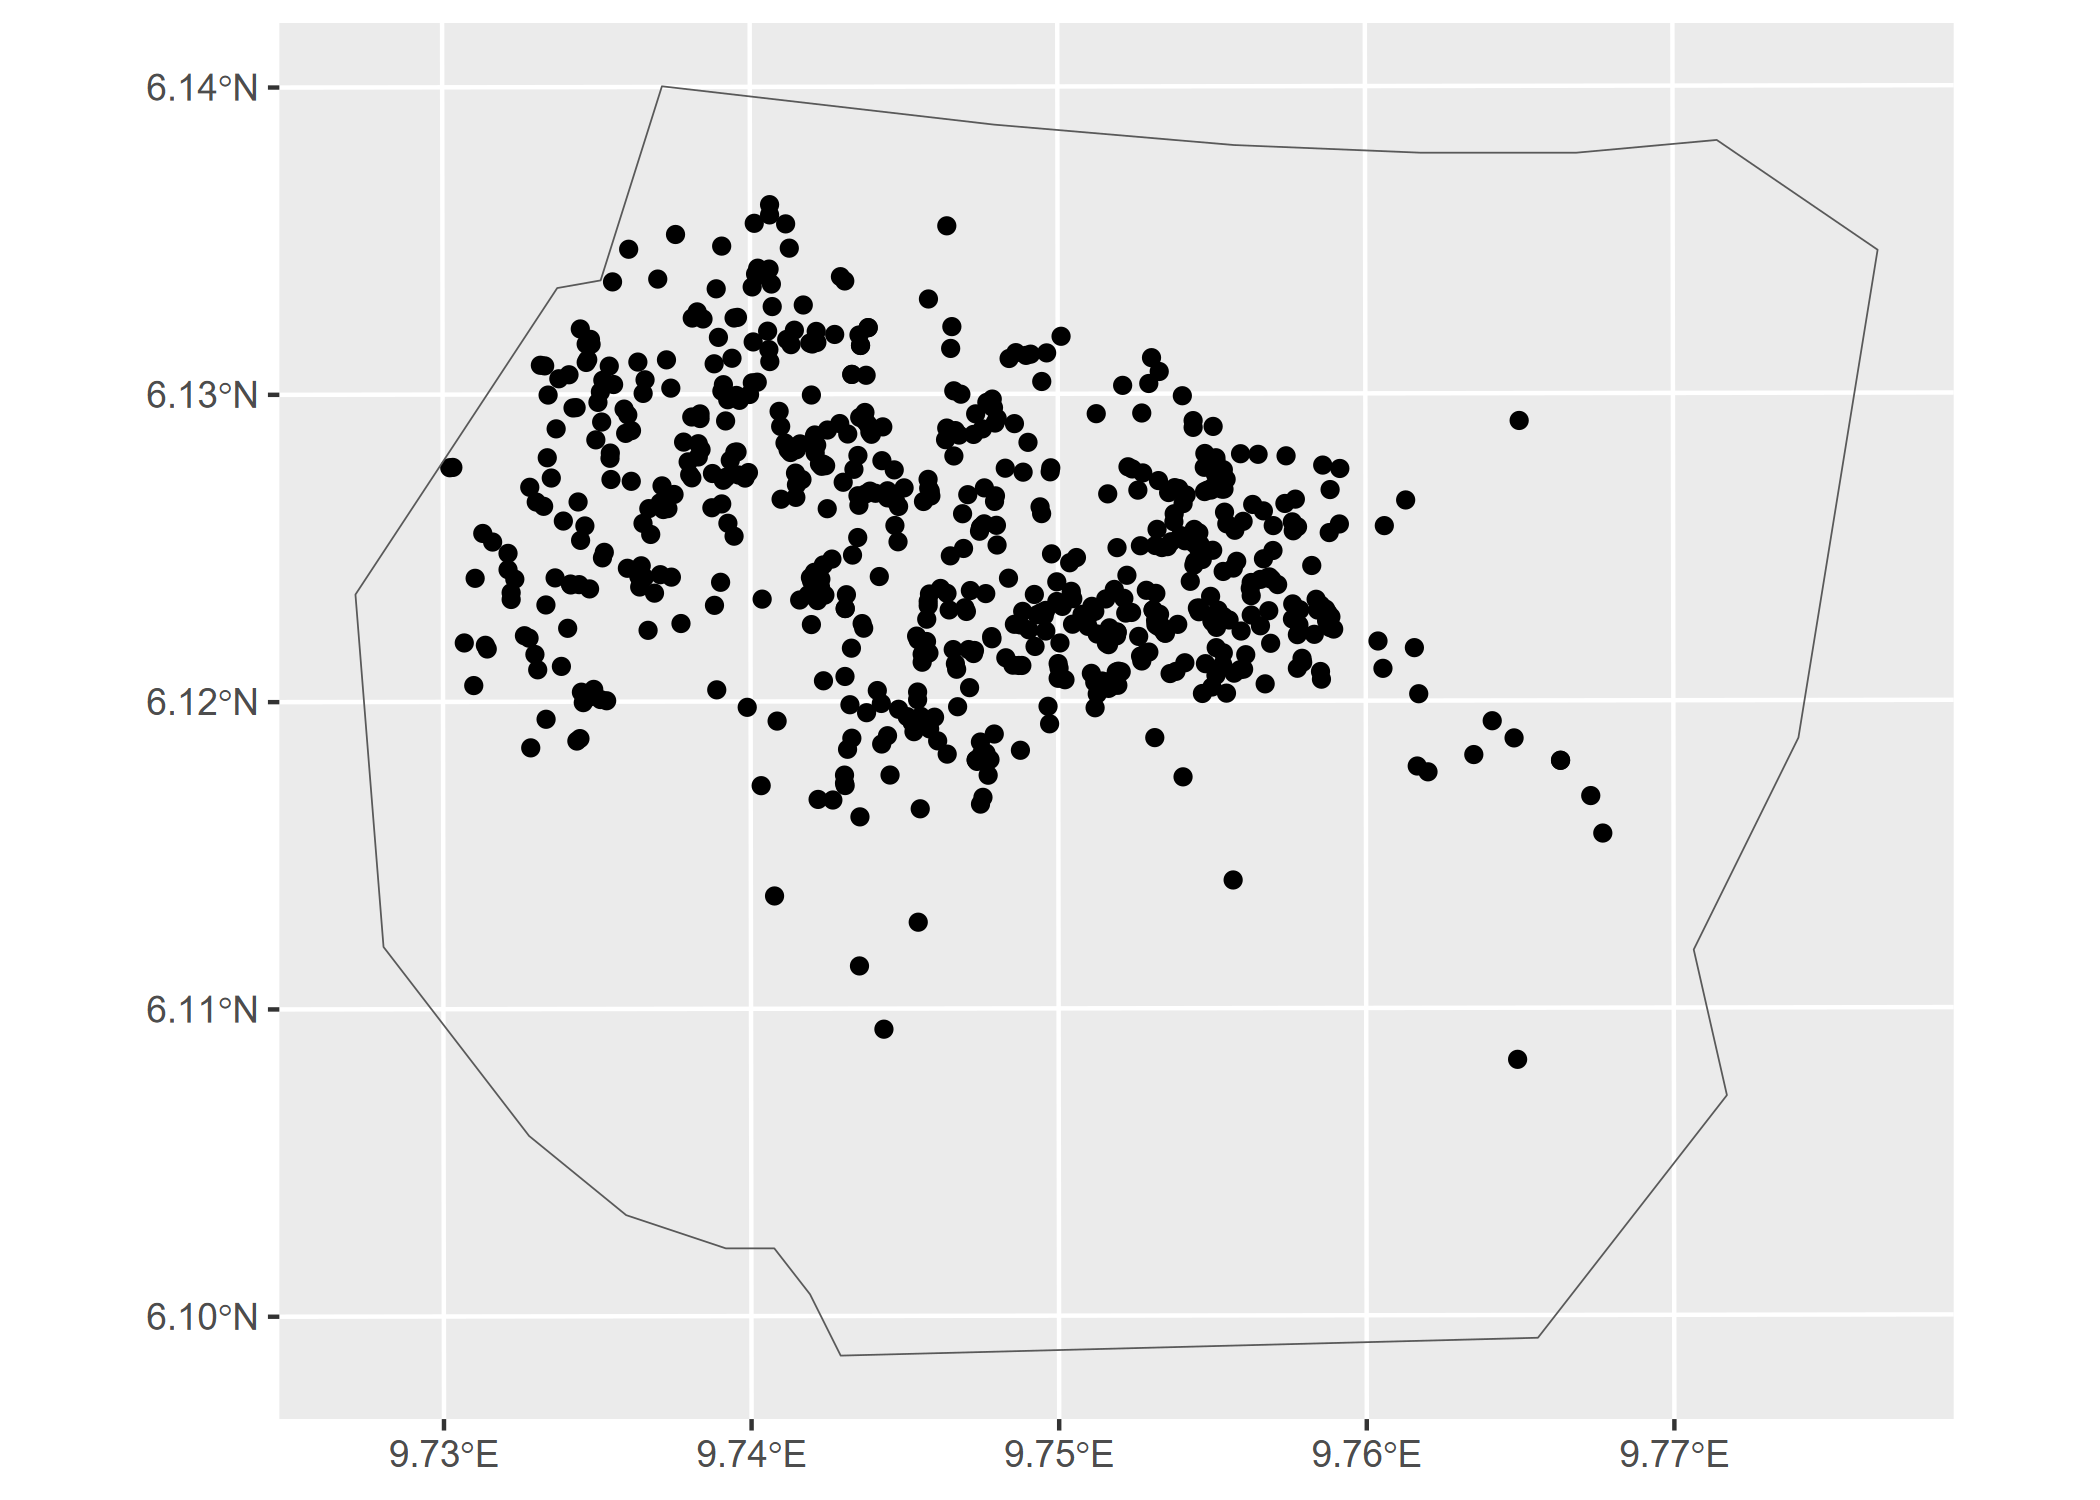
\includegraphics[width=0.8\linewidth,height=\textheight,keepaspectratio]{day5_practical_8_files/figure-pdf/nests_loc-1.png}

}

\caption{Location of gorilla nests}

\end{figure}%

:::

The dataset also contains covariates in the form or raster data. We
consider two of them here: ::: \{.cell\}

\begin{Shaded}
\begin{Highlighting}[]
\NormalTok{gcov }\OtherTok{=} \FunctionTok{gorillas\_sf\_gcov}\NormalTok{()}
\NormalTok{elev\_cov }\OtherTok{\textless{}{-}}\NormalTok{ gcov}\SpecialCharTok{$}\NormalTok{elevation}
\NormalTok{dist\_cov }\OtherTok{\textless{}{-}}\NormalTok{  gcov}\SpecialCharTok{$}\NormalTok{waterdist}
\end{Highlighting}
\end{Shaded}

:::

\begin{figure}[H]

{\centering 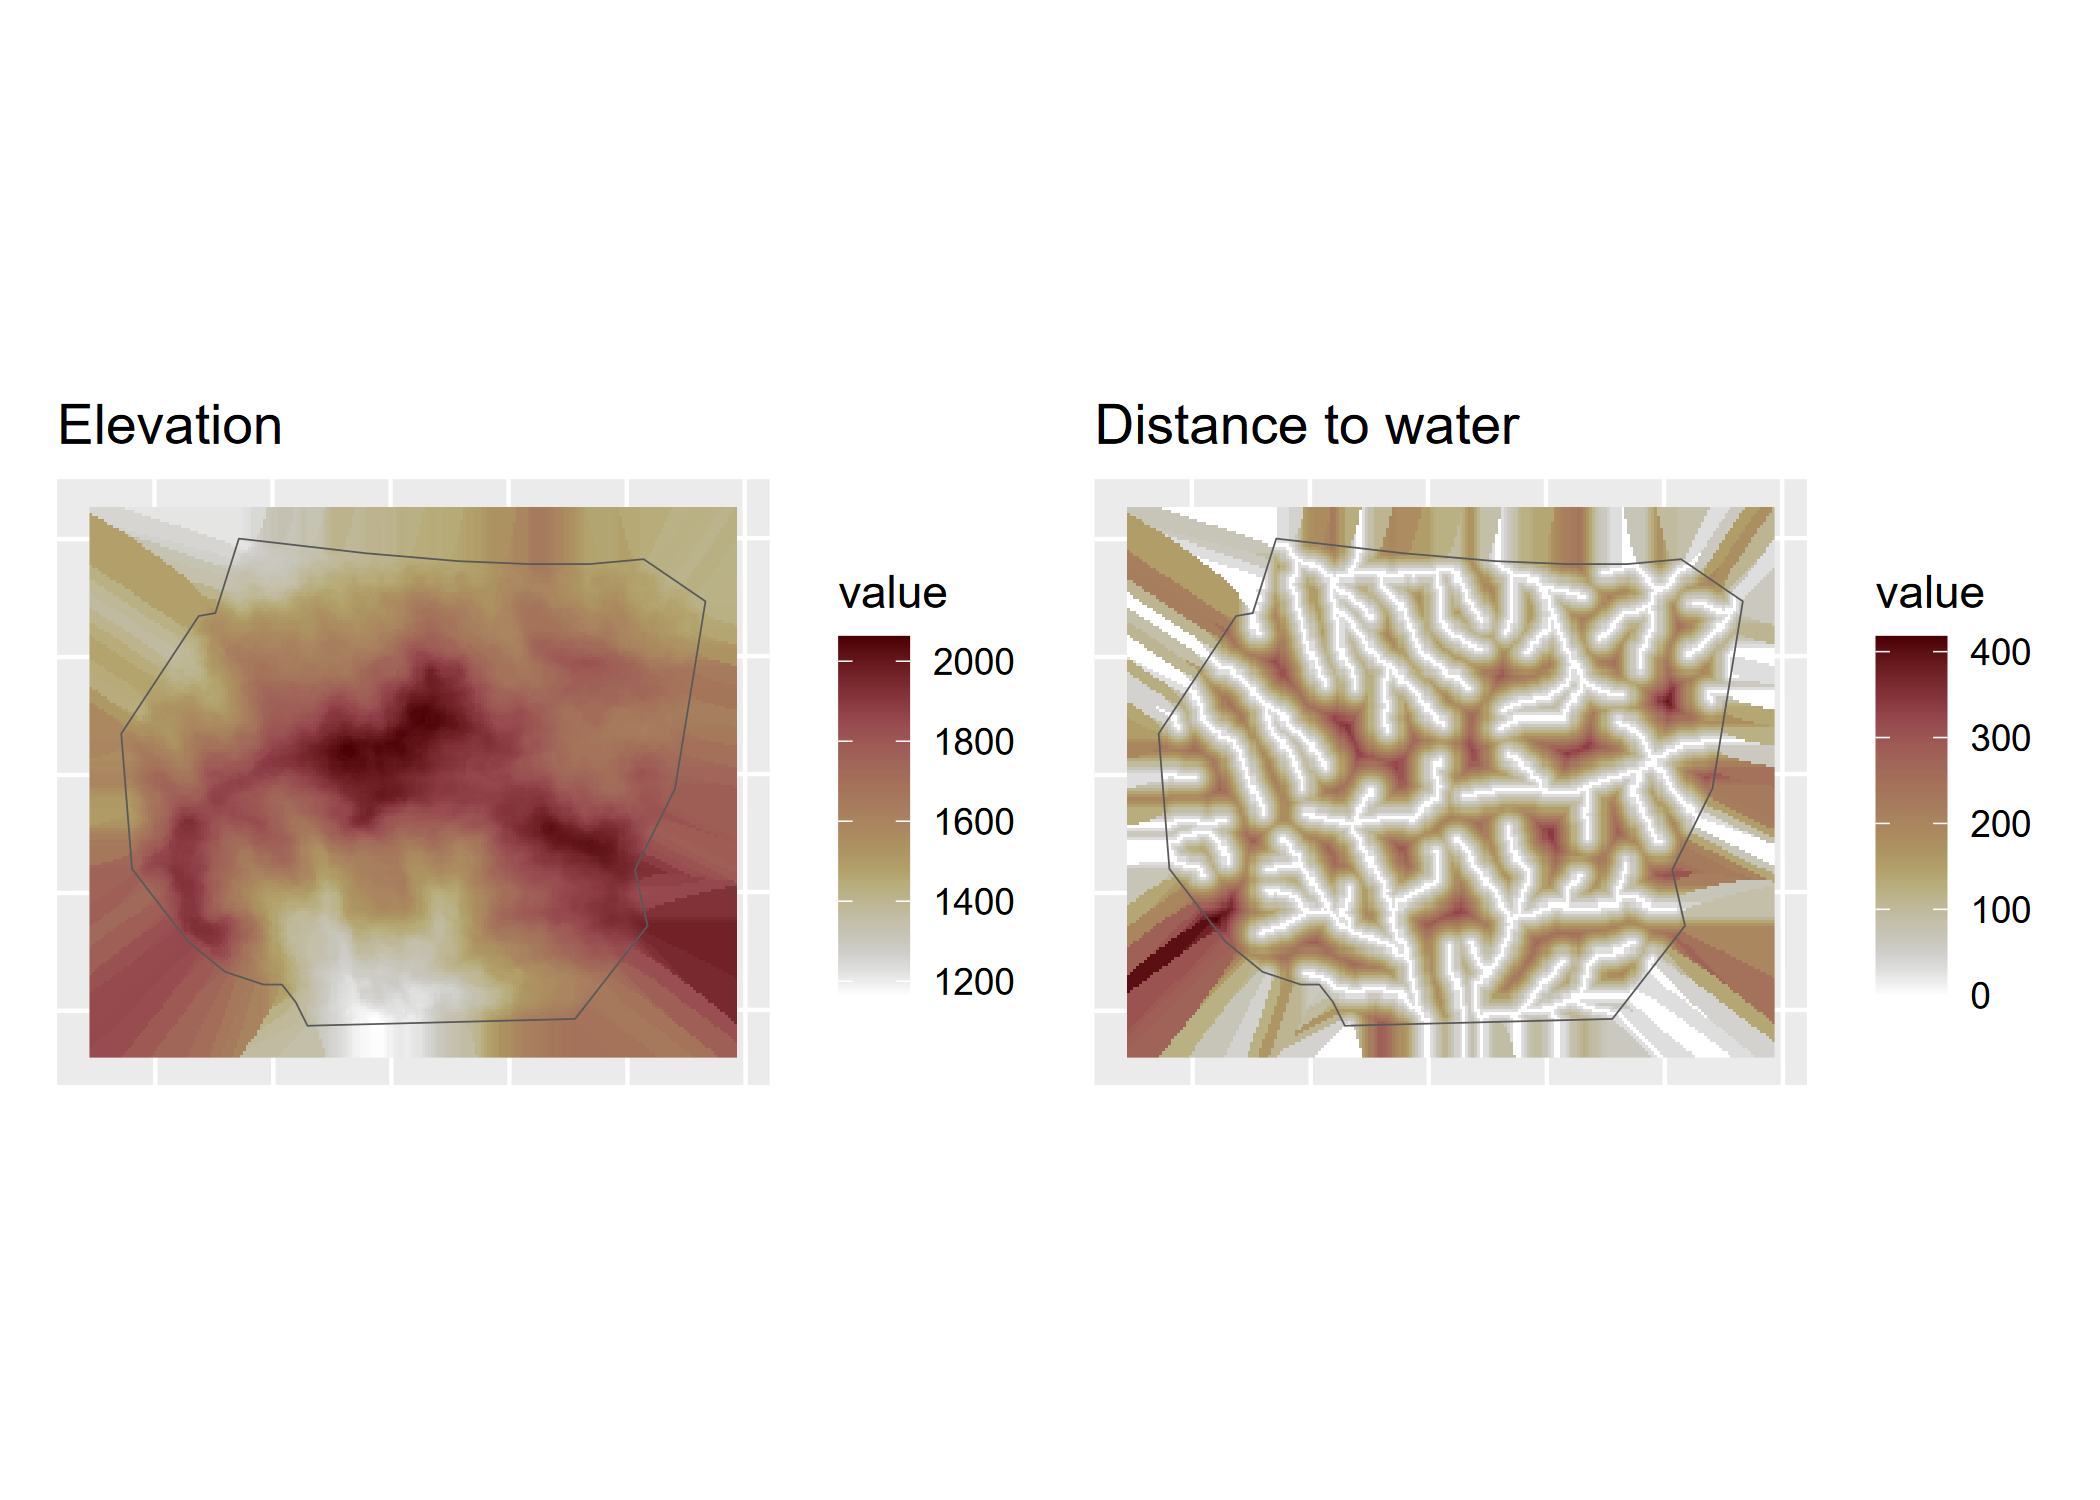
\includegraphics[width=0.8\linewidth,height=\textheight,keepaspectratio]{day5_practical_8_files/figure-pdf/unnamed-chunk-64-1.png}

}

\caption{Covariates}

\end{figure}%

\textbf{Note:} the covariates have been expanded to cover all the nodes
in the mesh.

\begin{center}\rule{0.5\linewidth}{0.5pt}\end{center}

To obtain the count data, we rasterize the species counts to match the
spatial resolution of the covariates available. Then we aggregate the
pixels to a rougher resolution (5x5 pixels in the original covariate
raster dimensions). Finally, we mask regions outside the study area.

In addition we compute the area of each grid cell.

\begin{Shaded}
\begin{Highlighting}[]
\CommentTok{\# Rasterize data}
\NormalTok{counts\_rstr }\OtherTok{\textless{}{-}}
\NormalTok{  terra}\SpecialCharTok{::}\FunctionTok{rasterize}\NormalTok{(}\FunctionTok{vect}\NormalTok{(nests), gcov, }\AttributeTok{fun =}\NormalTok{ sum, }\AttributeTok{background =} \DecValTok{0}\NormalTok{) }\SpecialCharTok{\%\textgreater{}\%}
\NormalTok{  terra}\SpecialCharTok{::}\FunctionTok{aggregate}\NormalTok{(}\AttributeTok{fact =} \DecValTok{5}\NormalTok{, }\AttributeTok{fun =}\NormalTok{ sum) }\SpecialCharTok{\%\textgreater{}\%}
  \FunctionTok{mask}\NormalTok{(}\FunctionTok{vect}\NormalTok{(sf}\SpecialCharTok{::}\FunctionTok{st\_geometry}\NormalTok{(boundary)))}
\FunctionTok{plot}\NormalTok{(counts\_rstr)}
\end{Highlighting}
\end{Shaded}

\begin{figure}[H]

{\centering 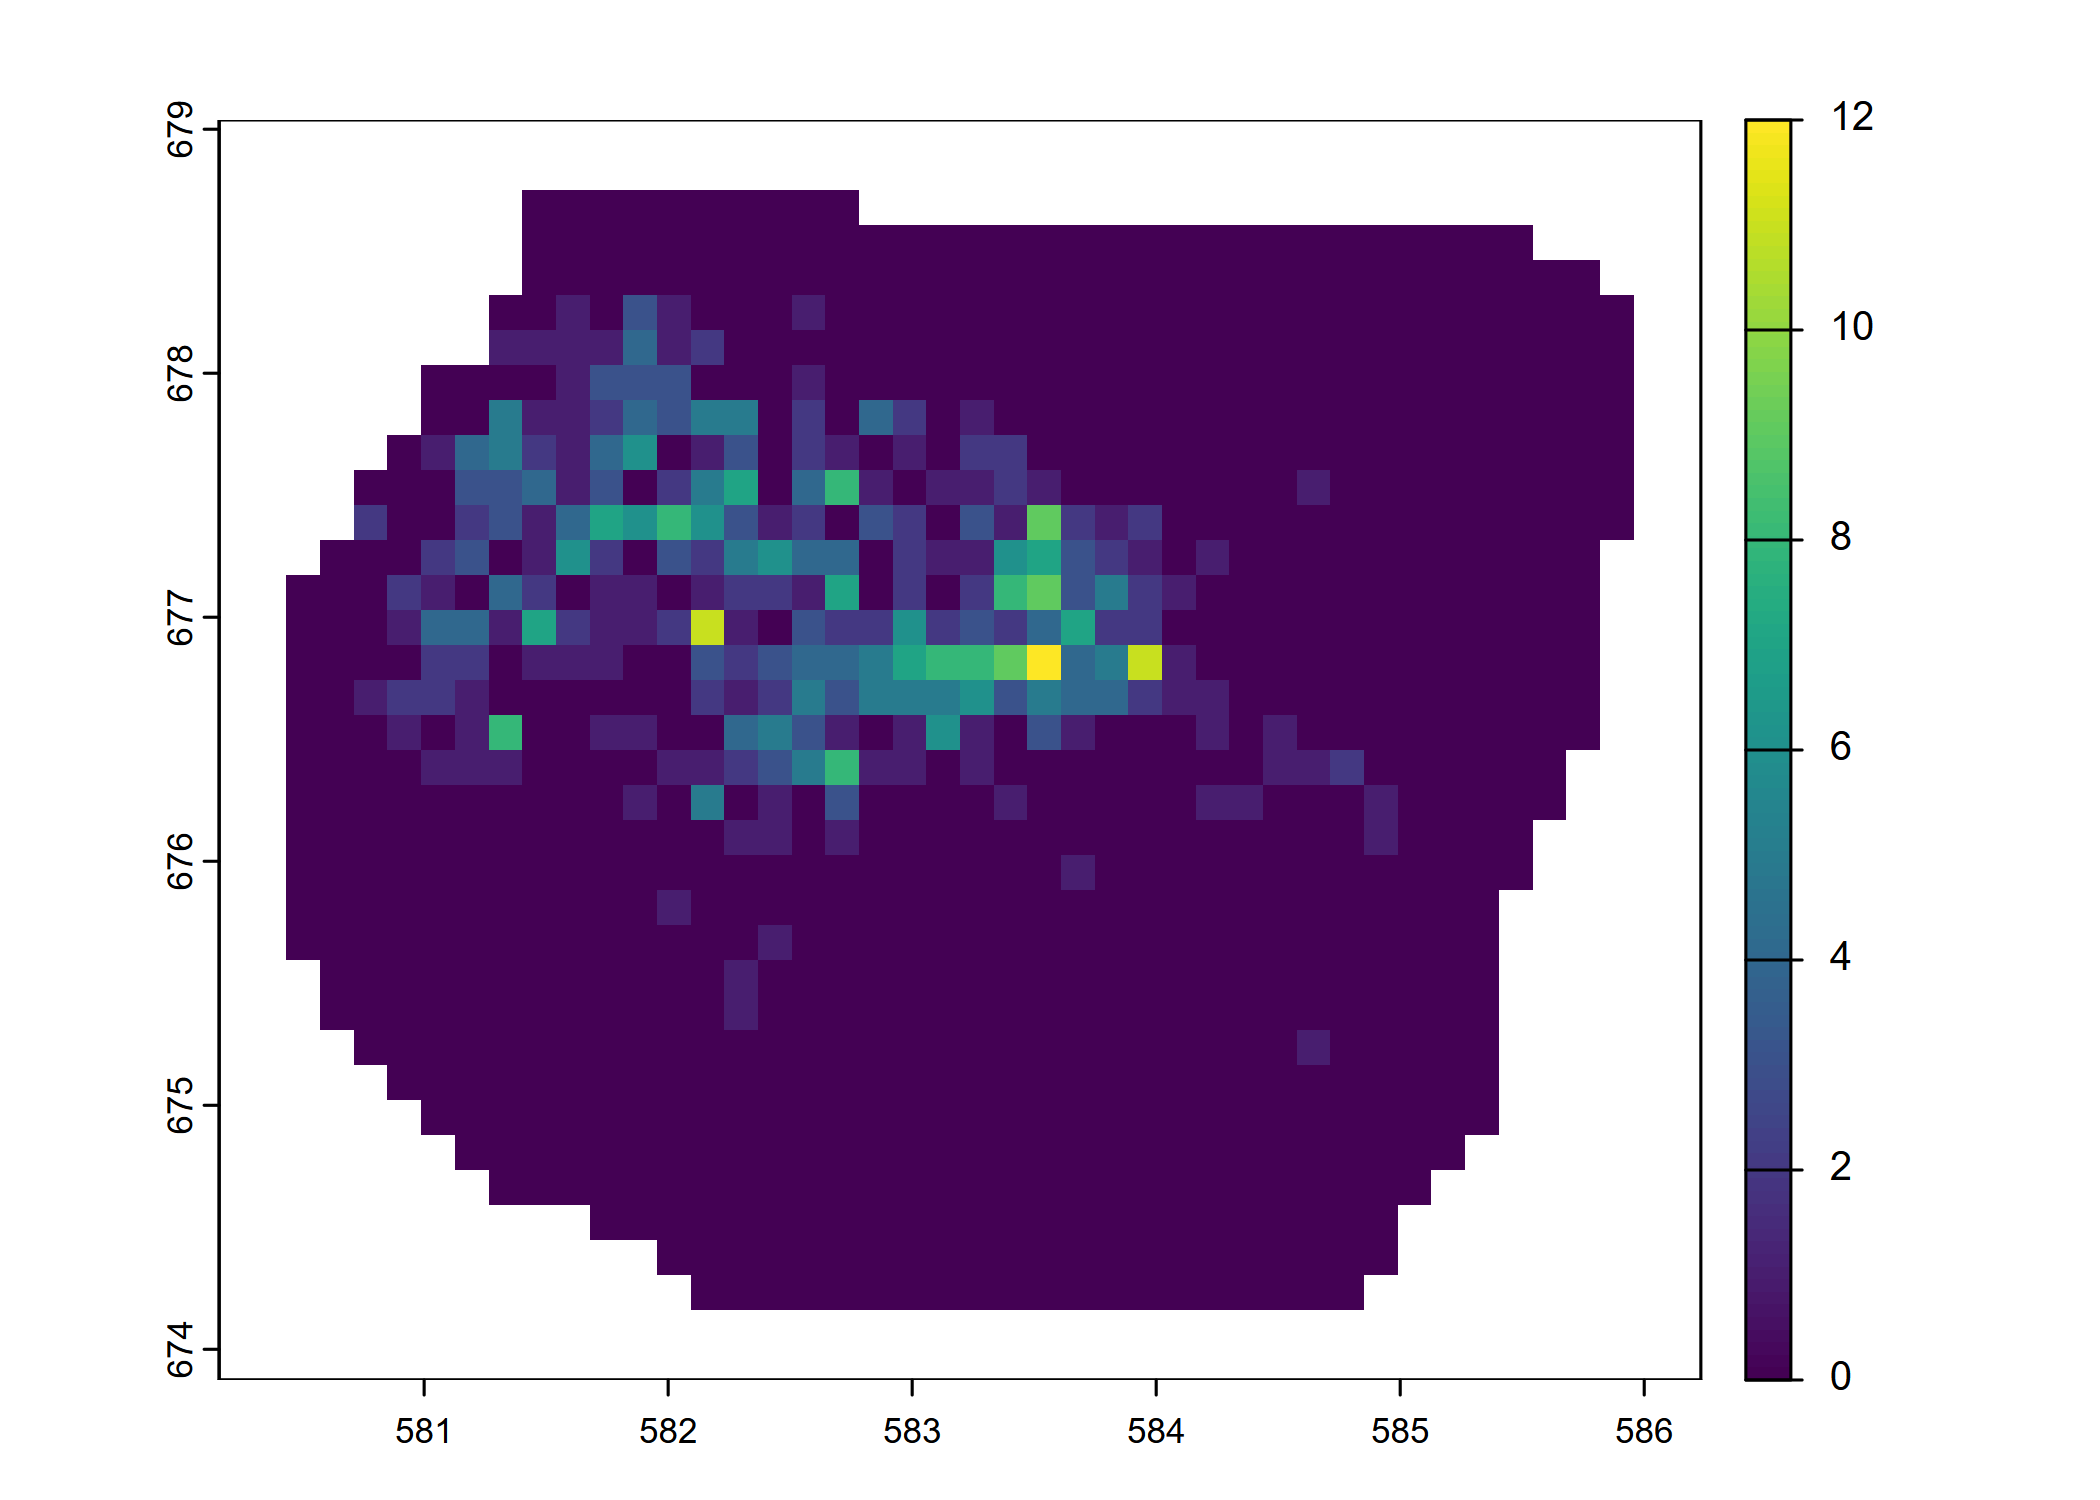
\includegraphics[width=0.8\linewidth,height=\textheight,keepaspectratio]{day5_practical_8_files/figure-pdf/unnamed-chunk-65-1.png}

}

\caption{Counts of gorilla nests}

\end{figure}%

\begin{Shaded}
\begin{Highlighting}[]
\CommentTok{\# compute cell area}
\NormalTok{counts\_rstr }\OtherTok{\textless{}{-}}\NormalTok{ counts\_rstr }\SpecialCharTok{\%\textgreater{}\%}
  \FunctionTok{cellSize}\NormalTok{(}\AttributeTok{unit =} \StringTok{"km"}\NormalTok{) }\SpecialCharTok{\%\textgreater{}\%}
  \FunctionTok{c}\NormalTok{(counts\_rstr)}
\end{Highlighting}
\end{Shaded}

To create our dataset of counts, we extract also the coordinate of
center point of each raster pixel. In addition we create a column with
presences and one with the pixel area

\begin{Shaded}
\begin{Highlighting}[]
\NormalTok{counts\_df }\OtherTok{\textless{}{-}} \FunctionTok{crds}\NormalTok{(counts\_rstr, }\AttributeTok{df =} \ConstantTok{TRUE}\NormalTok{, }\AttributeTok{na.rm =} \ConstantTok{TRUE}\NormalTok{) }\SpecialCharTok{\%\textgreater{}\%}
  \FunctionTok{bind\_cols}\NormalTok{(}\FunctionTok{values}\NormalTok{(counts\_rstr, }\AttributeTok{mat =} \ConstantTok{TRUE}\NormalTok{, }\AttributeTok{na.rm =} \ConstantTok{TRUE}\NormalTok{)) }\SpecialCharTok{\%\textgreater{}\%}
  \FunctionTok{rename}\NormalTok{(}\AttributeTok{count =}\NormalTok{ sum) }\SpecialCharTok{\%\textgreater{}\%}
  \FunctionTok{mutate}\NormalTok{(}\AttributeTok{present =}\NormalTok{ (count }\SpecialCharTok{\textgreater{}} \DecValTok{0}\NormalTok{) }\SpecialCharTok{*} \DecValTok{1}\NormalTok{L) }\SpecialCharTok{\%\textgreater{}\%}
  \FunctionTok{st\_as\_sf}\NormalTok{(}\AttributeTok{coords =} \FunctionTok{c}\NormalTok{(}\StringTok{"x"}\NormalTok{, }\StringTok{"y"}\NormalTok{), }\AttributeTok{crs =} \FunctionTok{st\_crs}\NormalTok{(nests))}
\end{Highlighting}
\end{Shaded}

We then aggregate the covariates to the same resolution as the nest
counts and scale them.

\begin{Shaded}
\begin{Highlighting}[]
\NormalTok{elev\_cov1 }\OtherTok{\textless{}{-}}\NormalTok{ elev\_cov }\SpecialCharTok{\%\textgreater{}\%} 
\NormalTok{  terra}\SpecialCharTok{::}\FunctionTok{aggregate}\NormalTok{(}\AttributeTok{fact =} \DecValTok{5}\NormalTok{, }\AttributeTok{fun =}\NormalTok{ mean) }\SpecialCharTok{\%\textgreater{}\%} \FunctionTok{scale}\NormalTok{()}
\NormalTok{dist\_cov1 }\OtherTok{\textless{}{-}}\NormalTok{ dist\_cov }\SpecialCharTok{\%\textgreater{}\%} 
\NormalTok{  terra}\SpecialCharTok{::}\FunctionTok{aggregate}\NormalTok{(}\AttributeTok{fact =} \DecValTok{5}\NormalTok{, }\AttributeTok{fun =}\NormalTok{ mean) }\SpecialCharTok{\%\textgreater{}\%} \FunctionTok{scale}\NormalTok{()}
\end{Highlighting}
\end{Shaded}

\begin{figure}

\centering{

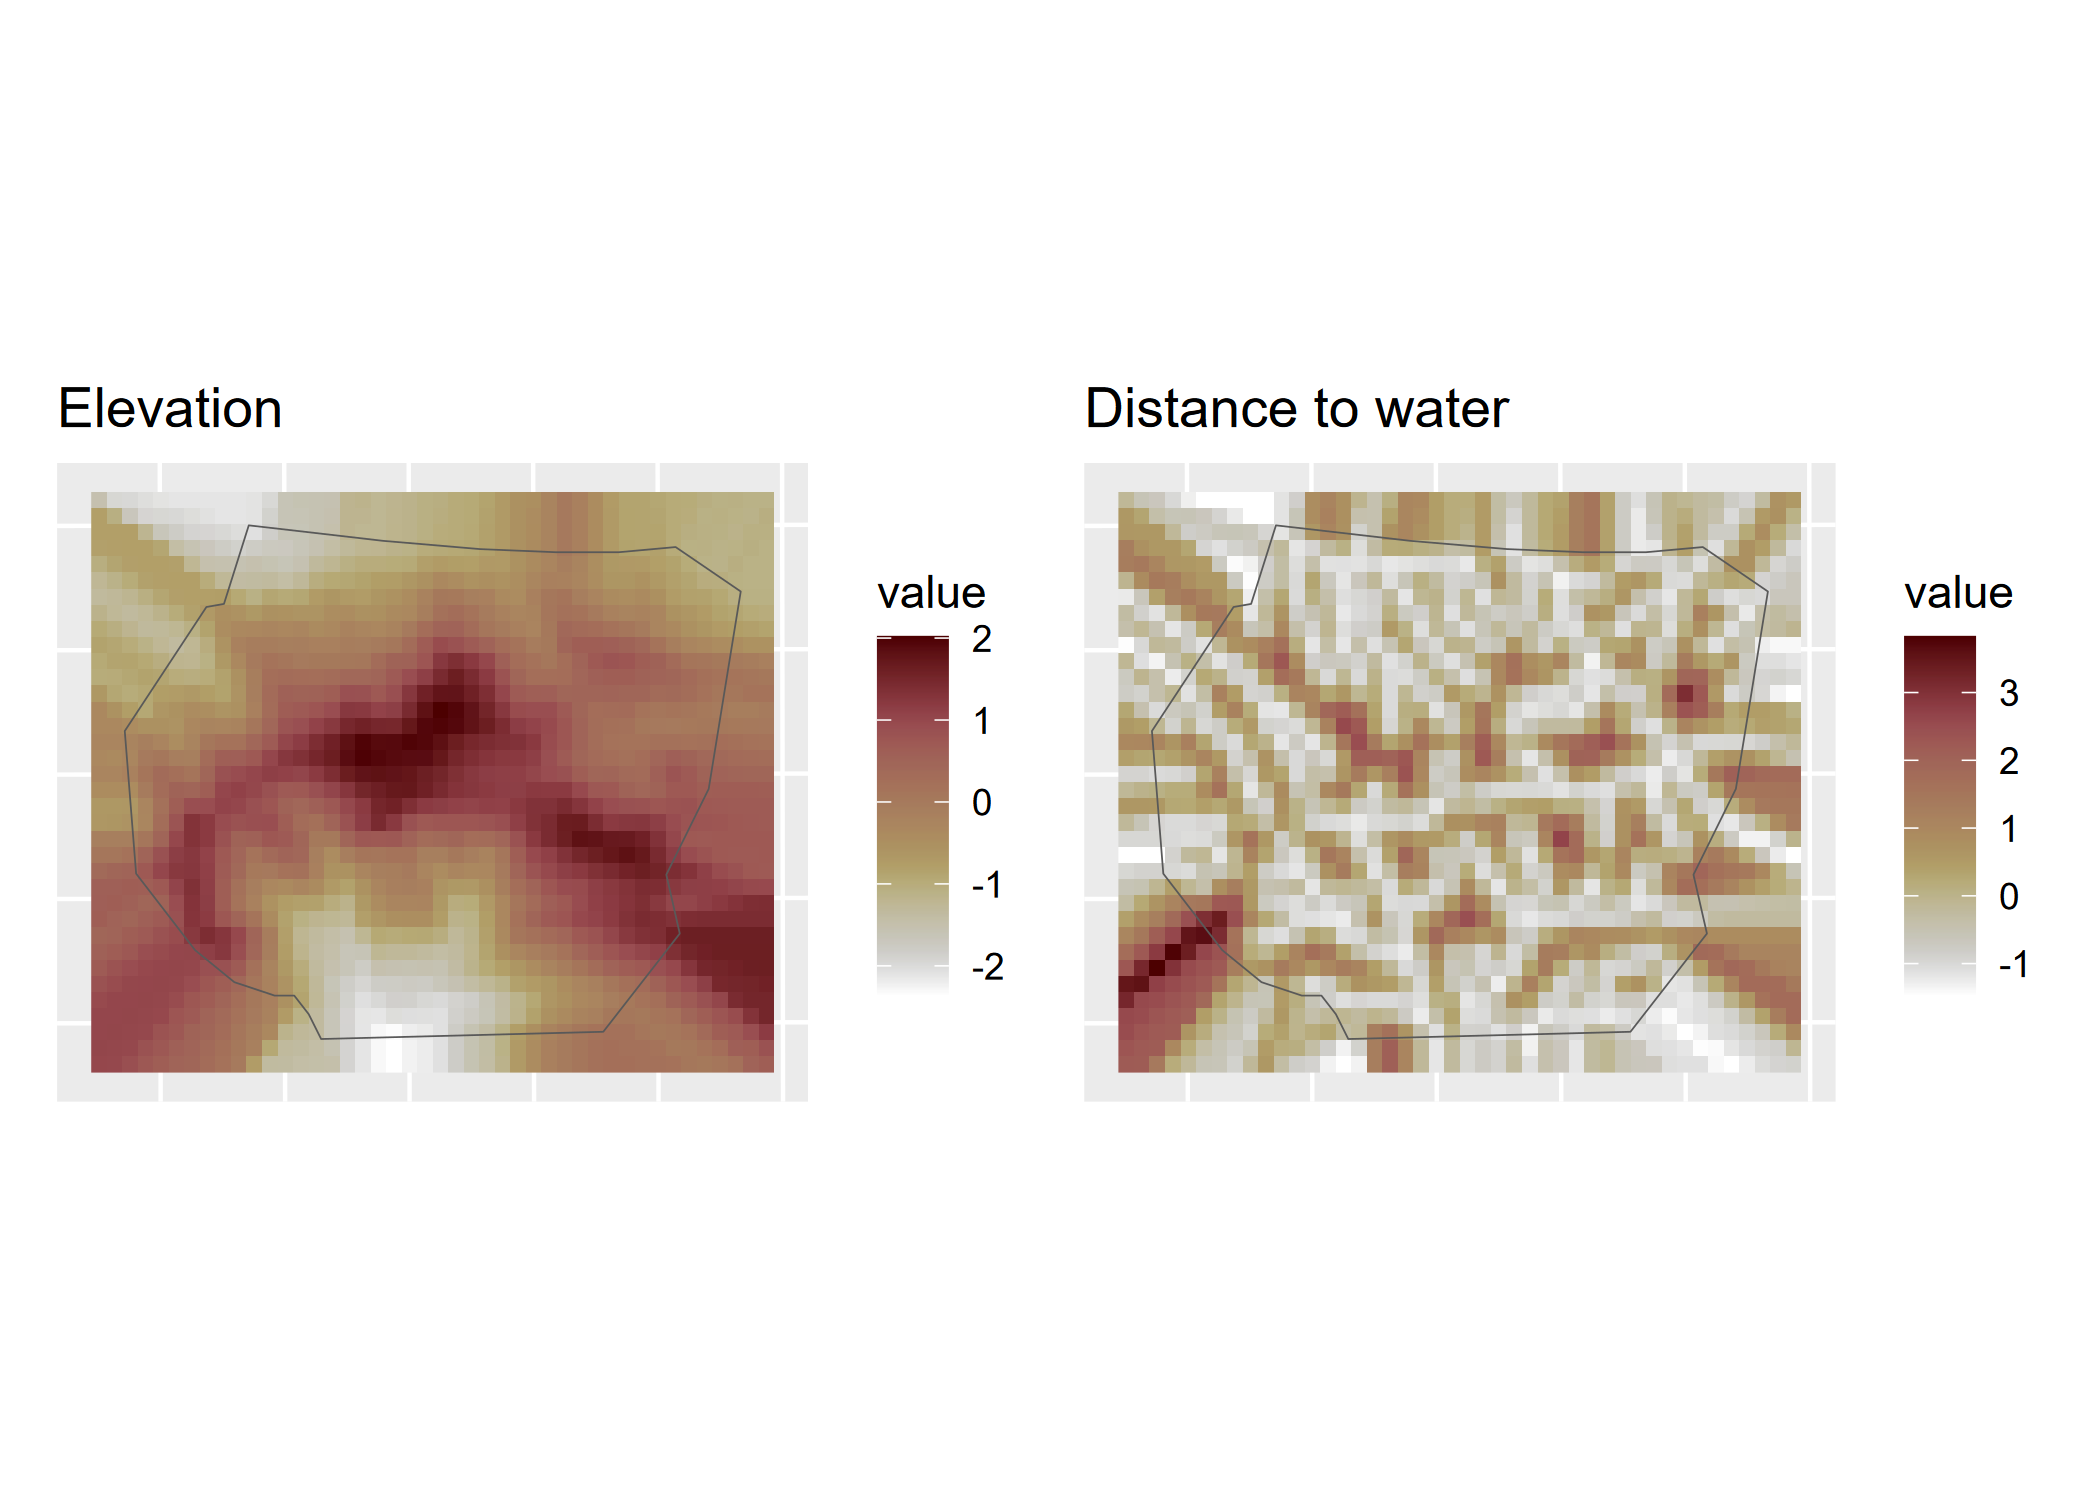
\includegraphics[width=0.8\linewidth,height=\textheight,keepaspectratio]{day5_practical_8_files/figure-pdf/fig-covariate-raster-1.png}

}

\caption{\label{fig-covariate-raster}Covariates}

\end{figure}%

\section{Mesh building}\label{mesh-building}

We now define the mesh and the spde object.

\begin{Shaded}
\begin{Highlighting}[]

\NormalTok{mesh }\OtherTok{\textless{}{-}} \FunctionTok{fm\_mesh\_2d}\NormalTok{(}
  \AttributeTok{loc =} \FunctionTok{st\_as\_sfc}\NormalTok{(counts\_df),}
  \AttributeTok{max.edge =} \FunctionTok{c}\NormalTok{(}\FloatTok{0.5}\NormalTok{, }\DecValTok{1}\NormalTok{),}
  \AttributeTok{crs =} \FunctionTok{st\_crs}\NormalTok{(counts\_df)}
\NormalTok{)}

\NormalTok{matern }\OtherTok{\textless{}{-}} \FunctionTok{inla.spde2.pcmatern}\NormalTok{(mesh,}
  \AttributeTok{prior.sigma =} \FunctionTok{c}\NormalTok{(}\DecValTok{1}\NormalTok{, }\FloatTok{0.01}\NormalTok{),}
  \AttributeTok{prior.range =} \FunctionTok{c}\NormalTok{(}\DecValTok{5}\NormalTok{, }\FloatTok{0.01}\NormalTok{)}
\NormalTok{)}
\end{Highlighting}
\end{Shaded}

\begin{figure}[H]

{\centering 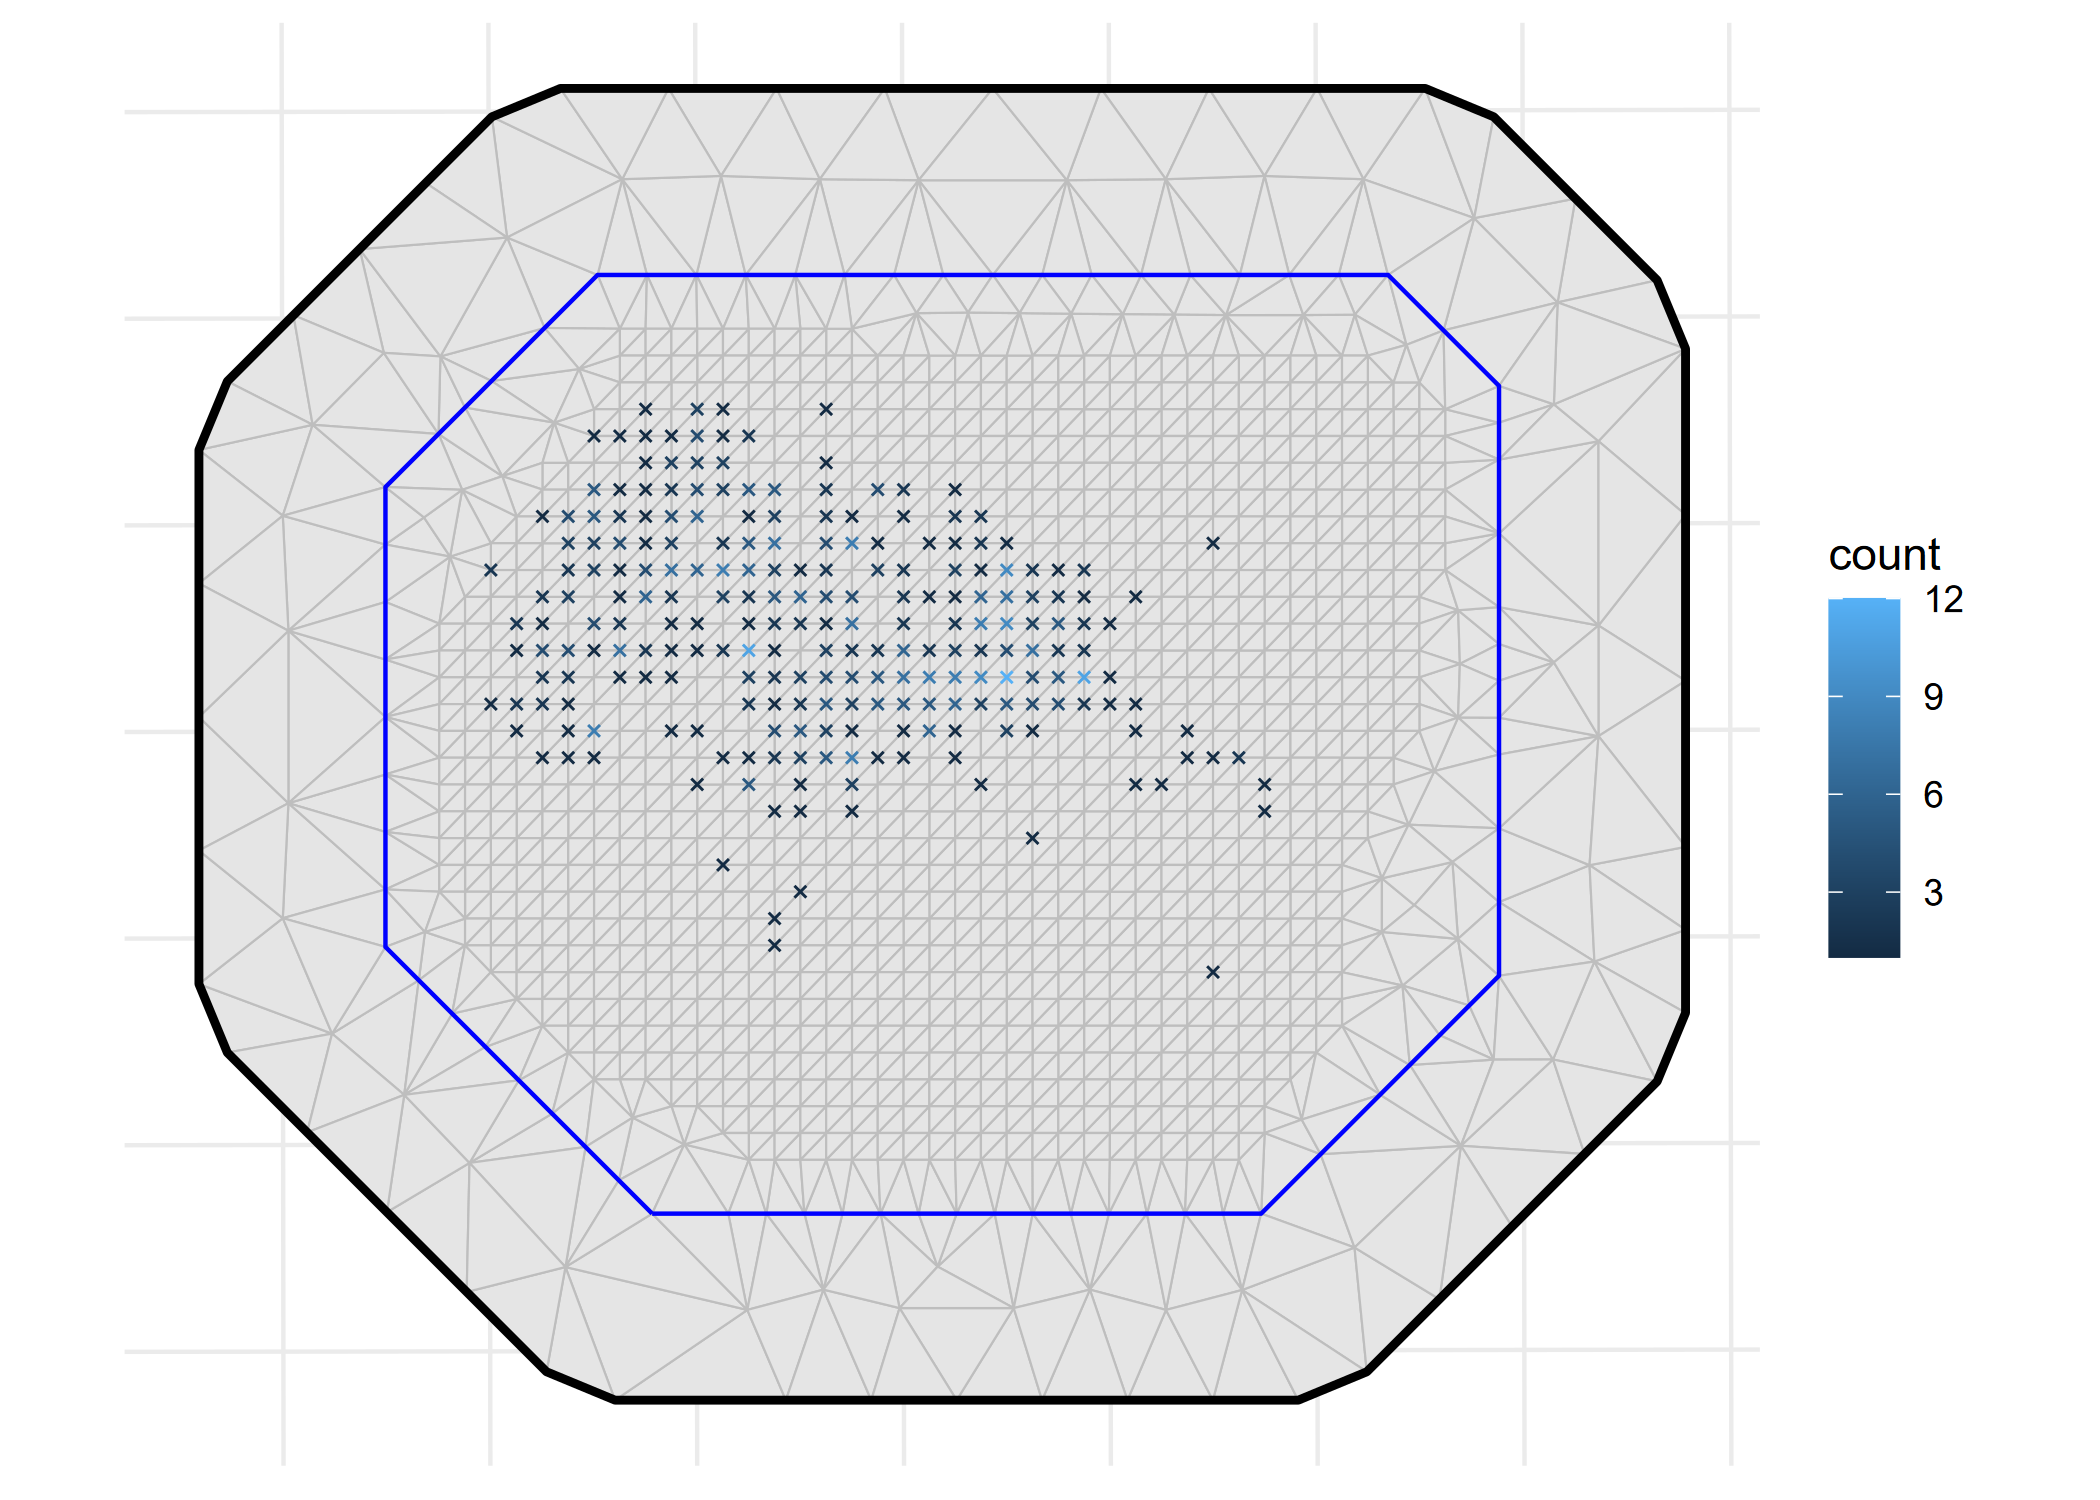
\includegraphics[width=0.8\linewidth,height=\textheight,keepaspectratio]{day5_practical_8_files/figure-pdf/unnamed-chunk-69-1.png}

}

\caption{Mesh over the count locations}

\end{figure}%

In our dataset, the number of zeros is quite substantial, and our model
may struggle to account for them adequately. To address this, we should
select a model capable of handling an ``inflated'' number of zeros,
exceeding what a standard Poisson model would imply. For this purpose,
we opt for a ``zero-inflated Poisson model,'' commonly abbreviated as
ZIP.

\section{Zero-Inflated model (Type1)}\label{sec-zip}

We fit now a Zero-Inflated model to our data.

The
\href{https://inla.r-inla-download.org/r-inla.org/doc/likelihood/zeroinflated.pdf}{Type
1 Zero-inflated Poisson model} is defined as follows:

\[
\text{Prob}(y\vert\dots)=\pi\times 1_{y=0}+(1-\pi)\times \text{Poisson}(y)
\]

Here, \(\pi=\text{logit}^{-1}(\theta)\)

The expected value and variance for the counts are calculated as:

\begin{equation}\phantomsection\label{eq-mean-zip}{
\begin{gathered}
E(count)=(1-\pi)\lambda \\
Var(count)= (1-\pi)(\lambda+\pi \lambda^2)
\end{gathered}
}\end{equation}

This model has two parameters:

\begin{itemize}
\tightlist
\item
  The probability of excess zero \(\pi\) - This is a
  \emph{hyperparameter} and therefore it is constant
\item
  The mean of the Poisson distribution \(\lambda\). This is linked to
  the linear predictor as: \[
  \eta = E\log(\lambda) = \log(E) + \beta_0 + \beta_1\text{Elevation} + \beta_2\text{Distance } + u
  \] where \(\log(E)\) is an offset (the area of the pixel) that
  accounts for the size of the cell.
\end{itemize}

\begin{tcolorbox}[enhanced jigsaw, colback=white, bottomrule=.15mm, arc=.35mm, opacitybacktitle=0.6, rightrule=.15mm, breakable, coltitle=black, toprule=.15mm, bottomtitle=1mm, toptitle=1mm, titlerule=0mm, left=2mm, leftrule=.75mm, title={Task}, opacityback=0, colframe=quarto-callout-warning-color-frame, colbacktitle=quarto-callout-warning-color!10!white]

Fit a zero-inflated model to the data (\texttt{zeroinflatedpoisson1}) by
completing the following code: ::: \{.cell\}

\begin{Shaded}
\begin{Highlighting}[]
\NormalTok{cmp }\OtherTok{=} \ErrorTok{\textasciitilde{}} \FunctionTok{Intercept}\NormalTok{(}\DecValTok{1}\NormalTok{) }\SpecialCharTok{+} \FunctionTok{elevation}\NormalTok{(...) }\SpecialCharTok{+} \FunctionTok{distance}\NormalTok{(...) }\SpecialCharTok{+} \FunctionTok{space}\NormalTok{(...)}

\NormalTok{lik }\OtherTok{=} \FunctionTok{bru\_obs}\NormalTok{(...,}
    \AttributeTok{E =}\NormalTok{ area)}

\NormalTok{fit\_zip }\OtherTok{\textless{}{-}} \FunctionTok{bru}\NormalTok{(cmp, lik)}
\end{Highlighting}
\end{Shaded}

\end{tcolorbox}

Take hint

The \texttt{E\ =\ area} is an offset that adjusts for the size of each
cell.

Click here to see the solution

\begin{Shaded}
\begin{Highlighting}[]

\NormalTok{cmp }\OtherTok{=} \ErrorTok{\textasciitilde{}} \FunctionTok{Intercept}\NormalTok{(}\DecValTok{1}\NormalTok{) }\SpecialCharTok{+} \FunctionTok{elevation}\NormalTok{(elev\_cov1, }\AttributeTok{model =} \StringTok{"linear"}\NormalTok{) }\SpecialCharTok{+} \FunctionTok{distance}\NormalTok{(dist\_cov1, }\AttributeTok{model =} \StringTok{"linear"}\NormalTok{) }\SpecialCharTok{+} \FunctionTok{space}\NormalTok{(geometry, }\AttributeTok{model =}\NormalTok{ matern)}



\NormalTok{lik }\OtherTok{=} \FunctionTok{bru\_obs}\NormalTok{(}\AttributeTok{formula =}\NormalTok{ count }\SpecialCharTok{\textasciitilde{}}\NormalTok{ .,}
    \AttributeTok{family =} \StringTok{"zeroinflatedpoisson1"}\NormalTok{, }
    \AttributeTok{data =}\NormalTok{ counts\_df,}
    \AttributeTok{E =}\NormalTok{ area)}

\NormalTok{fit\_zip }\OtherTok{\textless{}{-}} \FunctionTok{bru}\NormalTok{(cmp, lik)}
\end{Highlighting}
\end{Shaded}

:::

Once the model is fitted we can look at the results

\begin{tcolorbox}[enhanced jigsaw, colback=white, bottomrule=.15mm, arc=.35mm, opacitybacktitle=0.6, rightrule=.15mm, breakable, coltitle=black, toprule=.15mm, bottomtitle=1mm, toptitle=1mm, titlerule=0mm, left=2mm, leftrule=.75mm, title={Task}, opacityback=0, colframe=quarto-callout-warning-color-frame, colbacktitle=quarto-callout-warning-color!10!white]

Check what the estimated excess zero probaility is.

Use the \texttt{predict()} function to look at the estimated
\(\lambda(s)\) and mean count in Equation~\ref{eq-mean-zip}

Take hint

To get the right name for the hyperparameters to use in the
\texttt{predict()} function, you can use the function
\texttt{bru\_names()}.

Click here to see the solution

\begin{Shaded}
\begin{Highlighting}[]
\CommentTok{\# to check the estimated excess zero probability:}
\CommentTok{\# fit\_zip$summary.hyperpar}

\NormalTok{pred\_zip }\OtherTok{\textless{}{-}} \FunctionTok{predict}\NormalTok{(}
\NormalTok{  fit\_zip, }
\NormalTok{  counts\_df,}
  \SpecialCharTok{\textasciitilde{}}\NormalTok{ \{}
\NormalTok{    pi }\OtherTok{\textless{}{-}}\NormalTok{ zero\_probability\_parameter\_for\_zero\_inflated\_poisson\_1}
\NormalTok{    lambda }\OtherTok{\textless{}{-}}\NormalTok{ area }\SpecialCharTok{*} \FunctionTok{exp}\NormalTok{( distance }\SpecialCharTok{+}\NormalTok{ elevation }\SpecialCharTok{+}\NormalTok{ space }\SpecialCharTok{+}\NormalTok{ Intercept)}
\NormalTok{    expect }\OtherTok{\textless{}{-}}\NormalTok{ (}\DecValTok{1}\SpecialCharTok{{-}}\NormalTok{pi) }\SpecialCharTok{*}\NormalTok{ lambda}
\NormalTok{    variance }\OtherTok{\textless{}{-}}\NormalTok{ (}\DecValTok{1}\SpecialCharTok{{-}}\NormalTok{pi) }\SpecialCharTok{*}\NormalTok{ (lambda }\SpecialCharTok{+}\NormalTok{ pi }\SpecialCharTok{*}\NormalTok{ lambda}\SpecialCharTok{\^{}}\DecValTok{2}\NormalTok{)}
    \FunctionTok{list}\NormalTok{(}
      \AttributeTok{lambda =}\NormalTok{ lambda,}
      \AttributeTok{expect =}\NormalTok{ expect,}
      \AttributeTok{variance =}\NormalTok{ variance}
\NormalTok{    )}
\NormalTok{  \},}
  \AttributeTok{n.samples =} \DecValTok{2500}
\NormalTok{)}
\end{Highlighting}
\end{Shaded}

\end{tcolorbox}

\begin{figure}[H]

{\centering 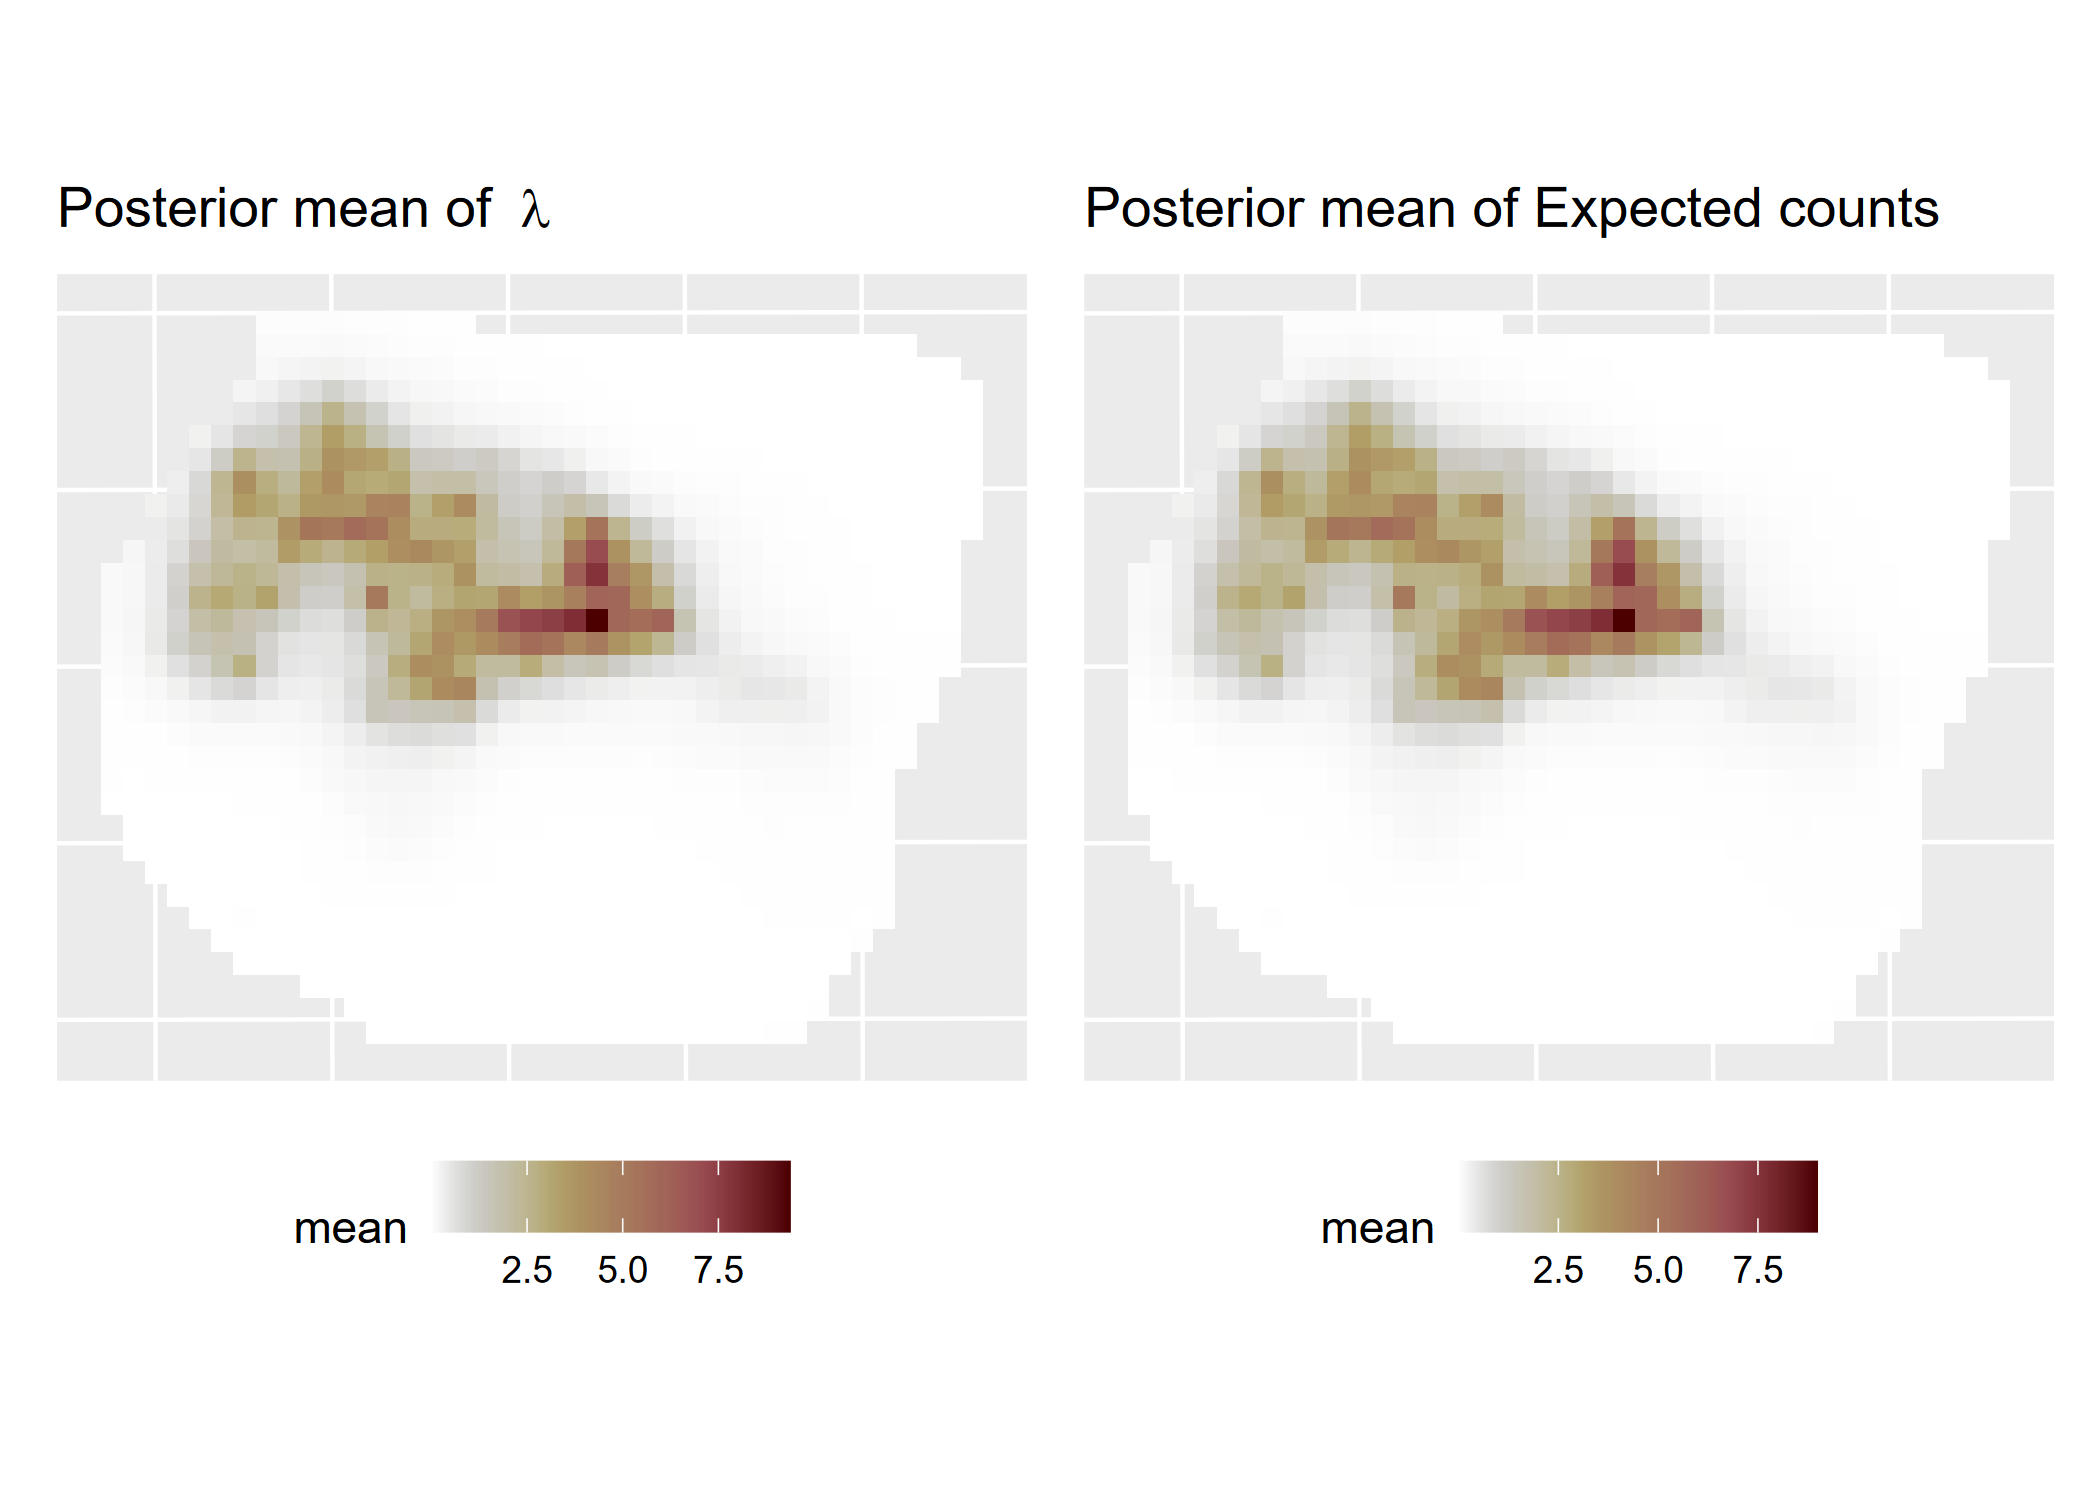
\includegraphics[width=0.8\linewidth,height=\textheight,keepaspectratio]{day5_practical_8_files/figure-pdf/unnamed-chunk-73-1.png}

}

\caption{Estimated \(\lambda\) (left) and expected counts (right) with
zero inflated model}

\end{figure}%

\section{Hurdle model (Type0)}\label{sec-zap}

We now fit a hurdle model to the same data.

In the \texttt{zeroinflatedpoisson0} model is defined by the
\href{https://inla.r-inla-download.org/r-inla.org/doc/likelihood/zeroinflated.pdf}{following
observation probability model}

\[
\text{Prob}(y\vert\dots)=\pi\times 1_{y=0}+(1-\pi)\times \text{Poisson}(y\vert y>0)
\]

where \(\pi\) is the probability of zero.

The expectation and variance of the counts are as follows:

\begin{equation}\phantomsection\label{eq-mean-zap}{
\begin{aligned}
E(\text{count})&=\frac{1}{1-\exp(-\lambda)}\pi\lambda \\
Var(\text{count})&=  E(\text{count}) \left(1-\exp(-\lambda) E(\text{count})\right)
\end{aligned}
}\end{equation}

\begin{tcolorbox}[enhanced jigsaw, colback=white, bottomrule=.15mm, arc=.35mm, opacitybacktitle=0.6, rightrule=.15mm, breakable, coltitle=black, toprule=.15mm, bottomtitle=1mm, toptitle=1mm, titlerule=0mm, left=2mm, leftrule=.75mm, title={Task}, opacityback=0, colframe=quarto-callout-warning-color-frame, colbacktitle=quarto-callout-warning-color!10!white]

Fit a hurdle model to the data using the \texttt{zeroinflatedpoisson0}
likelihood

Take hint

You do not need to redefine the components as the linear predictor is
not changing.

Click here to see the solution

\begin{Shaded}
\begin{Highlighting}[]
\NormalTok{lik }\OtherTok{=} \FunctionTok{bru\_obs}\NormalTok{(}\AttributeTok{formula =}\NormalTok{ count }\SpecialCharTok{\textasciitilde{}}\NormalTok{ .,}
    \AttributeTok{family =} \StringTok{"zeroinflatedpoisson0"}\NormalTok{, }
    \AttributeTok{data =}\NormalTok{ counts\_df,}
    \AttributeTok{E =}\NormalTok{ area)}

\NormalTok{fit\_zap }\OtherTok{\textless{}{-}} \FunctionTok{bru}\NormalTok{(cmp, lik)}
\end{Highlighting}
\end{Shaded}

\end{tcolorbox}

\begin{tcolorbox}[enhanced jigsaw, colback=white, bottomrule=.15mm, arc=.35mm, opacitybacktitle=0.6, rightrule=.15mm, breakable, coltitle=black, toprule=.15mm, bottomtitle=1mm, toptitle=1mm, titlerule=0mm, left=2mm, leftrule=.75mm, title={Task}, opacityback=0, colframe=quarto-callout-warning-color-frame, colbacktitle=quarto-callout-warning-color!10!white]

As before, check what the estimated probability of zero is and use
\texttt{predict()} to obtain a map of the estimated mean counts in
Equation~\ref{eq-mean-zap} over the domain.

Take hint

Click here to see the solution

\begin{Shaded}
\begin{Highlighting}[]

\NormalTok{pred\_zap }\OtherTok{\textless{}{-}} \FunctionTok{predict}\NormalTok{( fit\_zap, counts\_df,}
  \SpecialCharTok{\textasciitilde{}}\NormalTok{ \{}
\NormalTok{    pi }\OtherTok{\textless{}{-}}\NormalTok{ zero\_probability\_parameter\_for\_zero\_inflated\_poisson\_0}
\NormalTok{    lambda }\OtherTok{\textless{}{-}}\NormalTok{ area }\SpecialCharTok{*} \FunctionTok{exp}\NormalTok{( distance }\SpecialCharTok{+}\NormalTok{ elevation }\SpecialCharTok{+}\NormalTok{ space }\SpecialCharTok{+}\NormalTok{ Intercept)}
\NormalTok{    expect }\OtherTok{\textless{}{-}}\NormalTok{ ((}\DecValTok{1}\SpecialCharTok{{-}}\FunctionTok{exp}\NormalTok{(}\SpecialCharTok{{-}}\NormalTok{lambda))}\SpecialCharTok{\^{}}\NormalTok{(}\SpecialCharTok{{-}}\DecValTok{1}\NormalTok{) }\SpecialCharTok{*}\NormalTok{ pi }\SpecialCharTok{*}\NormalTok{ lambda)}
    \FunctionTok{list}\NormalTok{(}
      \AttributeTok{lambda =}\NormalTok{ lambda,}
      \AttributeTok{expect =}\NormalTok{ expect}
\NormalTok{    )}
\NormalTok{  \},}
  \AttributeTok{n.samples =} \DecValTok{2500}
\NormalTok{)}
\end{Highlighting}
\end{Shaded}

\end{tcolorbox}

\begin{figure}[H]

{\centering 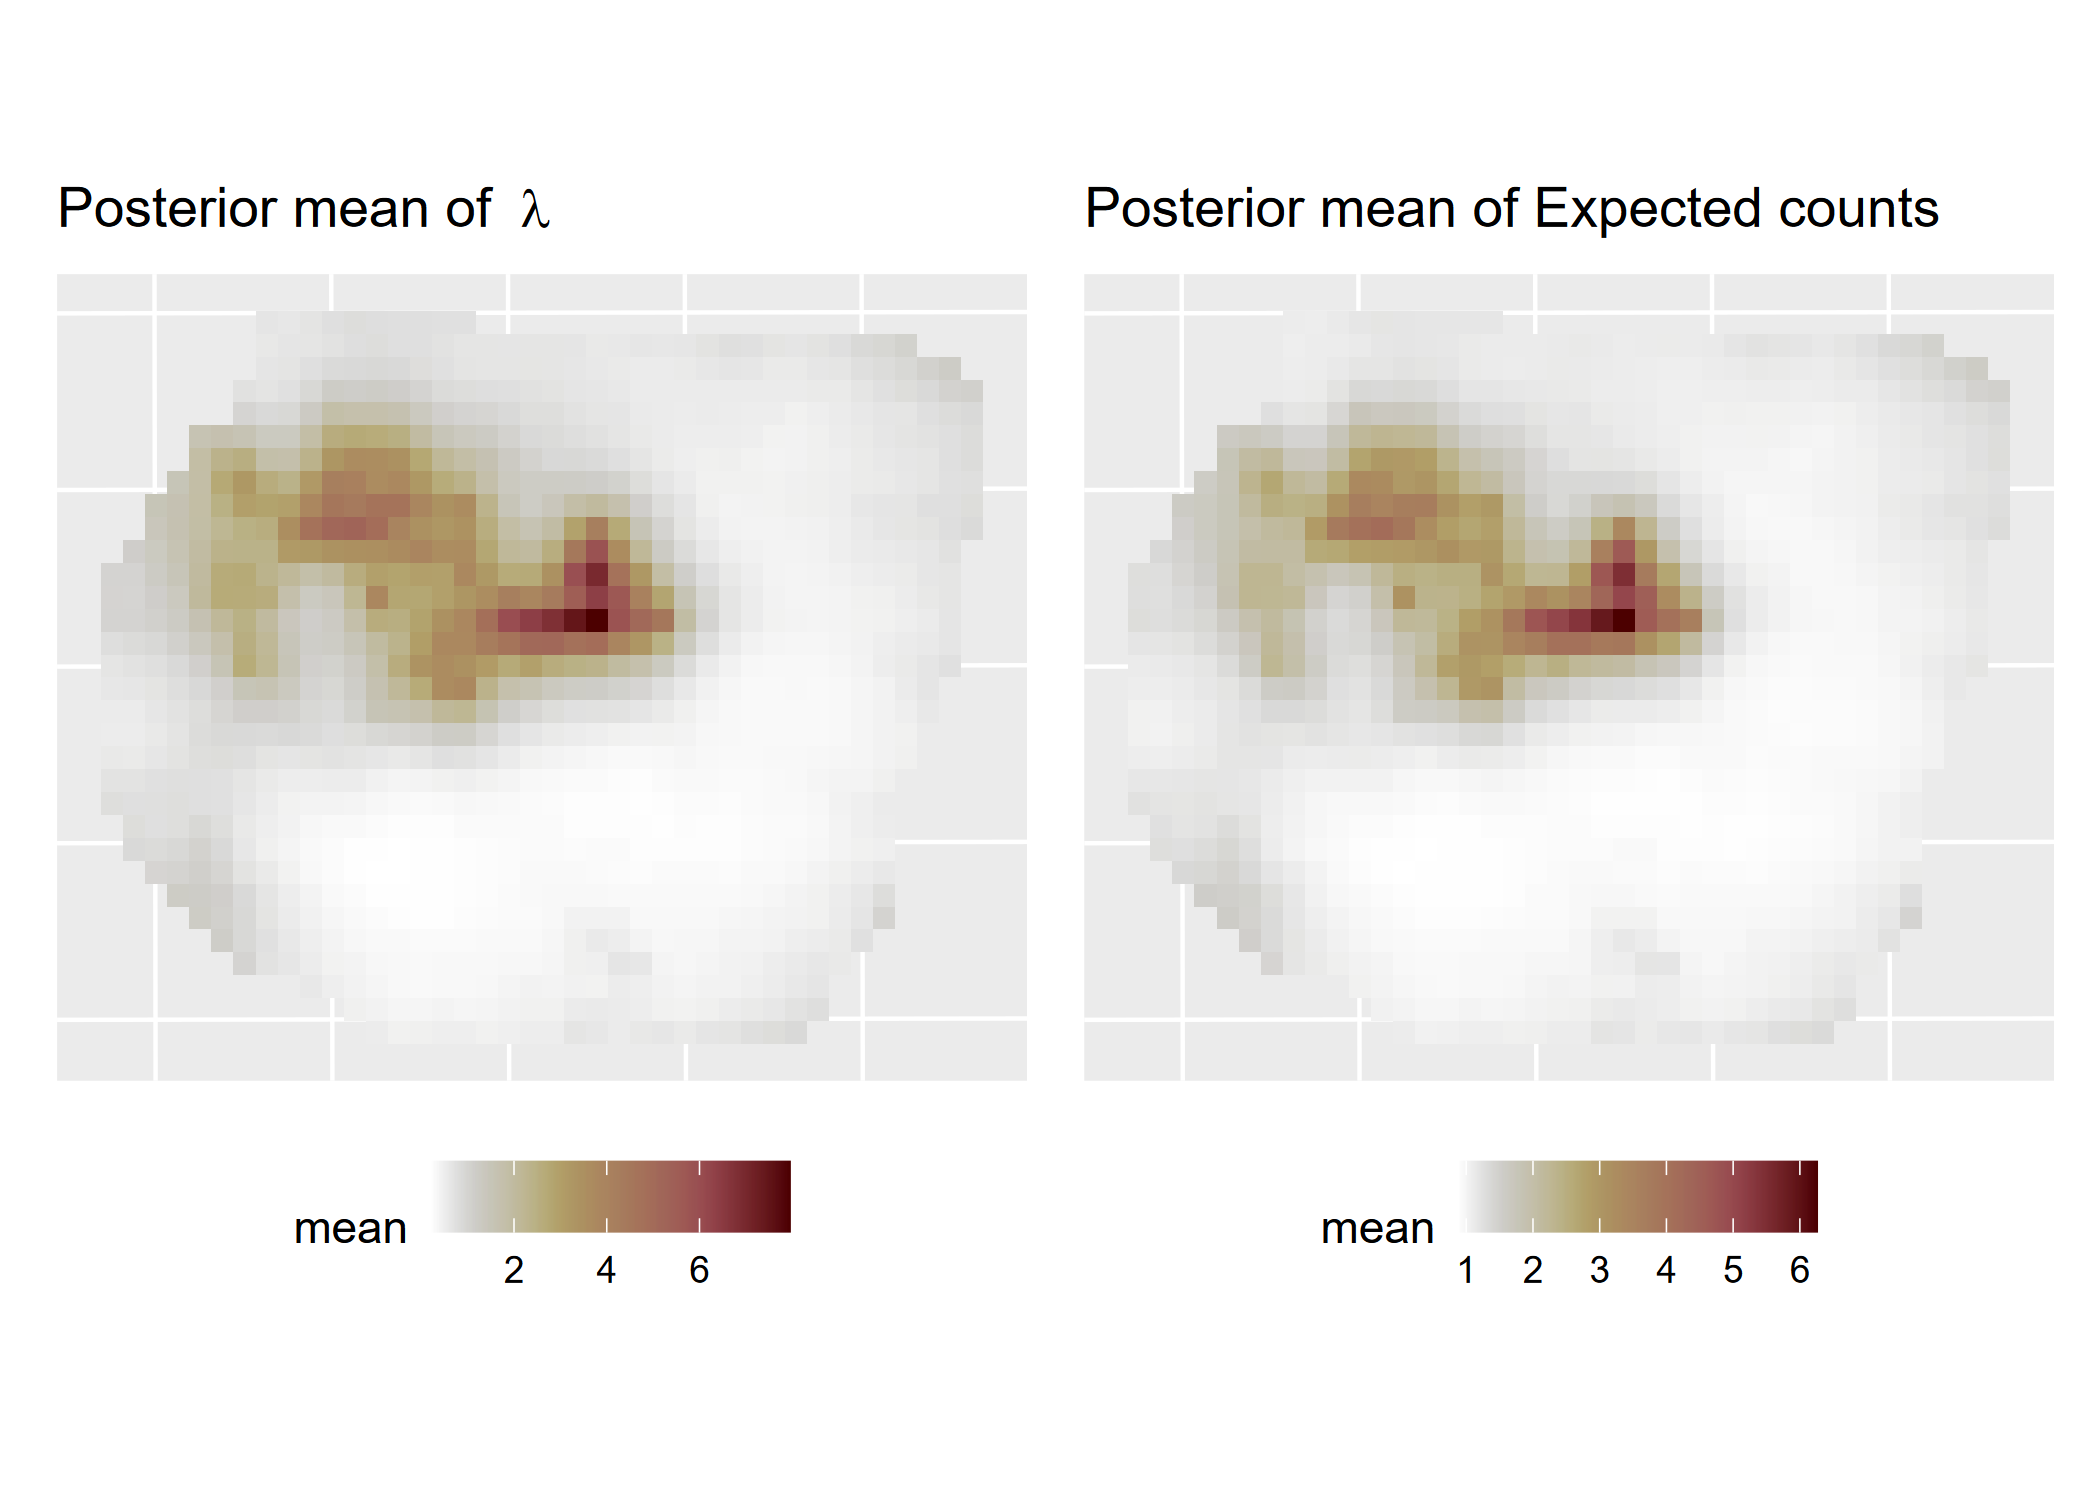
\includegraphics[width=0.8\linewidth,height=\textheight,keepaspectratio]{day5_practical_8_files/figure-pdf/unnamed-chunk-76-1.png}

}

\caption{Estimated \(\lambda\) (left) and expected counts (right) with
hurdle model}

\end{figure}%

\section{Hurdle model using two likelihoods}\label{sec-two-lik}

Here the model is the same as in Section~\ref{sec-zap}, but this time we
also want to model \(\pi\) using covariates and random effects.
Therefore we define a second linear predictor \[
\eta^2 =\beta_0^2 + \beta_1^2\text{Elevation} +  \beta_2^2\text{Distance} + u^2 
\] \textbf{Note} here we have defined the two linear predictor to use
the same covariates, but this is not necessary, they can be totally
independent.

To fit this model we have to define two likelihoods: - One will account
for the presence-absence process and has a Binomial model - One will
account for the counts and has a truncated Poisson model

\begin{tcolorbox}[enhanced jigsaw, colback=white, bottomrule=.15mm, arc=.35mm, opacitybacktitle=0.6, rightrule=.15mm, breakable, coltitle=black, toprule=.15mm, bottomtitle=1mm, toptitle=1mm, titlerule=0mm, left=2mm, leftrule=.75mm, title={Task}, opacityback=0, colframe=quarto-callout-warning-color-frame, colbacktitle=quarto-callout-warning-color!10!white]

Complete the following code to fit a hurdle model based on two
likelihoods:

\begin{Shaded}
\begin{Highlighting}[]
\CommentTok{\# define components}
\NormalTok{cmp }\OtherTok{\textless{}{-}} \ErrorTok{\textasciitilde{}}
  \FunctionTok{Intercept\_count}\NormalTok{(}\DecValTok{1}\NormalTok{) }\SpecialCharTok{+}
    \FunctionTok{elev\_count}\NormalTok{(elev\_cov1, }\AttributeTok{model =} \StringTok{"linear"}\NormalTok{) }\SpecialCharTok{+}
    \FunctionTok{dist\_count}\NormalTok{(dist\_cov1, }\AttributeTok{model =} \StringTok{"linear"}\NormalTok{) }\SpecialCharTok{+}
    \FunctionTok{space\_count}\NormalTok{(geometry, }\AttributeTok{model =}\NormalTok{ matern) }\SpecialCharTok{+}
    \FunctionTok{Intercept\_presence}\NormalTok{(}\DecValTok{1}\NormalTok{) }\SpecialCharTok{+}
    \FunctionTok{elev\_presence}\NormalTok{(elev\_cov1, }\AttributeTok{model =} \StringTok{"linear"}\NormalTok{) }\SpecialCharTok{+}
    \FunctionTok{dist\_presence}\NormalTok{(dist\_cov1, }\AttributeTok{model =} \StringTok{"linear"}\NormalTok{) }\SpecialCharTok{+}
    \FunctionTok{space\_presence}\NormalTok{(geometry, }\AttributeTok{model =}\NormalTok{ matern) }

\CommentTok{\# positive count model}
\NormalTok{pos\_count\_obs }\OtherTok{\textless{}{-}} \FunctionTok{bru\_obs}\NormalTok{(}\AttributeTok{formula =}\NormalTok{ ...,}
      \AttributeTok{family =}\NormalTok{ ...,}
      \AttributeTok{data =}\NormalTok{ counts\_df[counts\_df}\SpecialCharTok{$}\NormalTok{present }\SpecialCharTok{\textgreater{}} \DecValTok{0}\NormalTok{, ],}
      \AttributeTok{E =}\NormalTok{ area)}
  
\CommentTok{\# presence model}
\NormalTok{presence\_obs }\OtherTok{\textless{}{-}} \FunctionTok{bru\_obs}\NormalTok{(formula ...,}
  \AttributeTok{family =}\NormalTok{ ...,}
  \AttributeTok{data =}\NormalTok{ counts\_df,}
\NormalTok{)}

\CommentTok{\# fit the model}
\NormalTok{fit\_zap2 }\OtherTok{\textless{}{-}} \FunctionTok{bru}\NormalTok{(...)}
\end{Highlighting}
\end{Shaded}

Take hint

Add hint details here\ldots{}

Click here to see the solution

\begin{Shaded}
\begin{Highlighting}[]
\NormalTok{cmp }\OtherTok{\textless{}{-}} \ErrorTok{\textasciitilde{}}
  \FunctionTok{Intercept\_count}\NormalTok{(}\DecValTok{1}\NormalTok{) }\SpecialCharTok{+}
    \FunctionTok{elev\_count}\NormalTok{(elev\_cov1, }\AttributeTok{model =} \StringTok{"linear"}\NormalTok{) }\SpecialCharTok{+}
    \FunctionTok{dist\_count}\NormalTok{(dist\_cov1, }\AttributeTok{model =} \StringTok{"linear"}\NormalTok{) }\SpecialCharTok{+}
    \FunctionTok{space\_count}\NormalTok{(geometry, }\AttributeTok{model =}\NormalTok{ matern) }\SpecialCharTok{+}
    \FunctionTok{Intercept\_presence}\NormalTok{(}\DecValTok{1}\NormalTok{) }\SpecialCharTok{+}
    \FunctionTok{elev\_presence}\NormalTok{(elev\_cov1, }\AttributeTok{model =} \StringTok{"linear"}\NormalTok{) }\SpecialCharTok{+}
    \FunctionTok{dist\_presence}\NormalTok{(dist\_cov1, }\AttributeTok{model =} \StringTok{"linear"}\NormalTok{) }\SpecialCharTok{+}
    \FunctionTok{space\_presence}\NormalTok{(geometry, }\AttributeTok{model =}\NormalTok{ matern) }


\NormalTok{pos\_count\_obs }\OtherTok{\textless{}{-}} \FunctionTok{bru\_obs}\NormalTok{(}\AttributeTok{formula =}\NormalTok{ count }\SpecialCharTok{\textasciitilde{}}\NormalTok{ Intercept\_count }\SpecialCharTok{+}\NormalTok{ elev\_count }\SpecialCharTok{+} 
\NormalTok{                                   dist\_count }\SpecialCharTok{+}\NormalTok{ space\_count,}
      \AttributeTok{family =} \StringTok{"nzpoisson"}\NormalTok{,}
      \AttributeTok{data =}\NormalTok{ counts\_df[counts\_df}\SpecialCharTok{$}\NormalTok{present }\SpecialCharTok{\textgreater{}} \DecValTok{0}\NormalTok{, ],}
      \AttributeTok{E =}\NormalTok{ area)}
  

\NormalTok{presence\_obs }\OtherTok{\textless{}{-}} \FunctionTok{bru\_obs}\NormalTok{(}\AttributeTok{formula =}\NormalTok{ present }\SpecialCharTok{\textasciitilde{}}\NormalTok{ Intercept\_presence }\SpecialCharTok{+}\NormalTok{ elev\_presence }\SpecialCharTok{+}\NormalTok{ dist\_presence }\SpecialCharTok{+}
\NormalTok{                          space\_presence,}
  \AttributeTok{family =} \StringTok{"binomial"}\NormalTok{,}
  \AttributeTok{data =}\NormalTok{ counts\_df,}
\NormalTok{)}

\NormalTok{fit\_zap2 }\OtherTok{\textless{}{-}} \FunctionTok{bru}\NormalTok{(}
\NormalTok{  cmp,}
\NormalTok{  presence\_obs,}
\NormalTok{  pos\_count\_obs}
\NormalTok{)}
\end{Highlighting}
\end{Shaded}

\end{tcolorbox}

\section{Hurdle model using two likelihoods and a shared
component}\label{sec-two-lik-share}

Note that in the model above, there is no direct link between the
parameters of the two observation parts, and we could estimate them
separately. However, the two likelihoods could share some of the
components; for example the \texttt{space\_count} component could be
used for both predictors. This would be possible using the \texttt{copy}
argument.

We would then need to define one component as
\texttt{space(geometry,\ model\ =\ matern)} and then a copy of it as
\texttt{space\_copy(geometry,\ copy\ =\ "space",\ fixed\ =\ FALSE)}.

The results from the model in \textbf{?@sec-sec-two-lik} show that the
estimated covariance parameters for the two fields are very different,
so it is probably not sensible to share the same component between the
two parts. We do it anyway to show an example:

\begin{Shaded}
\begin{Highlighting}[]
\NormalTok{cmp }\OtherTok{\textless{}{-}} \ErrorTok{\textasciitilde{}}
  \FunctionTok{Intercept\_count}\NormalTok{(}\DecValTok{1}\NormalTok{) }\SpecialCharTok{+}
    \FunctionTok{elev\_count}\NormalTok{(elev\_cov1, }\AttributeTok{model =} \StringTok{"linear"}\NormalTok{) }\SpecialCharTok{+}
    \FunctionTok{dist\_count}\NormalTok{(dist\_cov1, }\AttributeTok{model =} \StringTok{"linear"}\NormalTok{) }\SpecialCharTok{+}
    \FunctionTok{Intercept\_presence}\NormalTok{(}\DecValTok{1}\NormalTok{) }\SpecialCharTok{+}
    \FunctionTok{elev\_presence}\NormalTok{(elev\_cov1, }\AttributeTok{model =} \StringTok{"linear"}\NormalTok{) }\SpecialCharTok{+}
    \FunctionTok{dist\_presence}\NormalTok{(dist\_cov1, }\AttributeTok{model =} \StringTok{"linear"}\NormalTok{) }\SpecialCharTok{+}
    \FunctionTok{space}\NormalTok{(geometry, }\AttributeTok{model =}\NormalTok{ matern) }\SpecialCharTok{+}
  \FunctionTok{space\_copy}\NormalTok{(geometry, }\AttributeTok{copy =} \StringTok{"space"}\NormalTok{, }\AttributeTok{fixed =} \ConstantTok{FALSE}\NormalTok{)}


\NormalTok{pos\_count\_obs }\OtherTok{\textless{}{-}} \FunctionTok{bru\_obs}\NormalTok{(}\AttributeTok{formula =}\NormalTok{ count }\SpecialCharTok{\textasciitilde{}}\NormalTok{ Intercept\_count }\SpecialCharTok{+}\NormalTok{ elev\_count }\SpecialCharTok{+}\NormalTok{ dist\_count }\SpecialCharTok{+}\NormalTok{ space,}
      \AttributeTok{family =} \StringTok{"nzpoisson"}\NormalTok{,}
      \AttributeTok{data =}\NormalTok{ counts\_df[counts\_df}\SpecialCharTok{$}\NormalTok{present }\SpecialCharTok{\textgreater{}} \DecValTok{0}\NormalTok{, ],}
      \AttributeTok{E =}\NormalTok{ area)}

\NormalTok{presence\_obs }\OtherTok{\textless{}{-}} \FunctionTok{bru\_obs}\NormalTok{(}\AttributeTok{formula =}\NormalTok{ present }\SpecialCharTok{\textasciitilde{}}\NormalTok{ Intercept\_presence }\SpecialCharTok{+}\NormalTok{ elev\_presence }\SpecialCharTok{+}\NormalTok{ dist\_presence }\SpecialCharTok{+}\NormalTok{ space\_copy,}
  \AttributeTok{family =} \StringTok{"binomial"}\NormalTok{,}
  \AttributeTok{data =}\NormalTok{ counts\_df)}

\NormalTok{fit\_zap3 }\OtherTok{\textless{}{-}} \FunctionTok{bru}\NormalTok{(}
\NormalTok{  cmp,}
\NormalTok{  presence\_obs,}
\NormalTok{  pos\_count\_obs)}
\end{Highlighting}
\end{Shaded}

\section{Comparing models}\label{comparing-models}

We have fitted four different models. Now we want to compare them and
see how they fit the data.

\subsection{Comparing model
predictions}\label{comparing-model-predictions}

We first want to compare the estimated surfaces of expected counts. To
do this we want to produce the estimated expected counts, similar to
what we did in Section~\ref{sec-zip} and Section~\ref{sec-zap} for all
four models and plot them together:

\begin{Shaded}
\begin{Highlighting}[]
\NormalTok{pred\_zip }\OtherTok{\textless{}{-}} \FunctionTok{predict}\NormalTok{(}
\NormalTok{  fit\_zip, }
\NormalTok{  counts\_df,}
  \SpecialCharTok{\textasciitilde{}}\NormalTok{ \{}
\NormalTok{    pi }\OtherTok{\textless{}{-}}\NormalTok{ zero\_probability\_parameter\_for\_zero\_inflated\_poisson\_1}
\NormalTok{    lambda }\OtherTok{\textless{}{-}}\NormalTok{ area }\SpecialCharTok{*} \FunctionTok{exp}\NormalTok{( distance }\SpecialCharTok{+}\NormalTok{ elevation }\SpecialCharTok{+}\NormalTok{ space }\SpecialCharTok{+}\NormalTok{ Intercept)}
\NormalTok{    expect }\OtherTok{\textless{}{-}}\NormalTok{ (}\DecValTok{1}\SpecialCharTok{{-}}\NormalTok{pi) }\SpecialCharTok{*}\NormalTok{ lambda}
\NormalTok{    variance }\OtherTok{\textless{}{-}}\NormalTok{ (}\DecValTok{1}\SpecialCharTok{{-}}\NormalTok{pi) }\SpecialCharTok{*}\NormalTok{ (lambda }\SpecialCharTok{+}\NormalTok{ pi }\SpecialCharTok{*}\NormalTok{ lambda}\SpecialCharTok{\^{}}\DecValTok{2}\NormalTok{)}
    \FunctionTok{list}\NormalTok{(}
      \AttributeTok{expect =}\NormalTok{ expect}
\NormalTok{    )}
\NormalTok{  \},}\AttributeTok{n.samples =} \DecValTok{2500}\NormalTok{)}

\NormalTok{pred\_zap }\OtherTok{\textless{}{-}} \FunctionTok{predict}\NormalTok{( fit\_zap, counts\_df,}
  \SpecialCharTok{\textasciitilde{}}\NormalTok{ \{}
\NormalTok{    pi }\OtherTok{\textless{}{-}}\NormalTok{ zero\_probability\_parameter\_for\_zero\_inflated\_poisson\_0}
\NormalTok{    lambda }\OtherTok{\textless{}{-}}\NormalTok{ area }\SpecialCharTok{*} \FunctionTok{exp}\NormalTok{( distance }\SpecialCharTok{+}\NormalTok{ elevation }\SpecialCharTok{+}\NormalTok{ space }\SpecialCharTok{+}\NormalTok{ Intercept)}
\NormalTok{    expect }\OtherTok{\textless{}{-}}\NormalTok{ ((}\DecValTok{1}\SpecialCharTok{{-}}\FunctionTok{exp}\NormalTok{(}\SpecialCharTok{{-}}\NormalTok{lambda))}\SpecialCharTok{\^{}}\NormalTok{(}\SpecialCharTok{{-}}\DecValTok{1}\NormalTok{) }\SpecialCharTok{*}\NormalTok{ pi }\SpecialCharTok{*}\NormalTok{ lambda)}
    \FunctionTok{list}\NormalTok{(}
      \AttributeTok{expect =}\NormalTok{ expect)}
\NormalTok{  \},}\AttributeTok{n.samples =} \DecValTok{2500}\NormalTok{)}

\NormalTok{inv.logit }\OtherTok{=} \ControlFlowTok{function}\NormalTok{(x) (}\FunctionTok{exp}\NormalTok{(x)}\SpecialCharTok{/}\NormalTok{(}\DecValTok{1}\SpecialCharTok{+}\FunctionTok{exp}\NormalTok{(x)))}

\NormalTok{pred\_zap2 }\OtherTok{\textless{}{-}} \FunctionTok{predict}\NormalTok{( fit\_zap2, counts\_df,}
  \SpecialCharTok{\textasciitilde{}}\NormalTok{ \{}
\NormalTok{    pi }\OtherTok{\textless{}{-}} \FunctionTok{inv.logit}\NormalTok{(Intercept\_presence }\SpecialCharTok{+}\NormalTok{ elev\_presence }\SpecialCharTok{+}\NormalTok{ dist\_presence }\SpecialCharTok{+}\NormalTok{ space\_presence)}
\NormalTok{    lambda }\OtherTok{\textless{}{-}}\NormalTok{ area }\SpecialCharTok{*} \FunctionTok{exp}\NormalTok{( dist\_count }\SpecialCharTok{+}\NormalTok{ elev\_count }\SpecialCharTok{+}\NormalTok{ space\_count }\SpecialCharTok{+}\NormalTok{ Intercept\_count)}
\NormalTok{    expect }\OtherTok{\textless{}{-}}\NormalTok{ ((}\DecValTok{1}\SpecialCharTok{{-}}\FunctionTok{exp}\NormalTok{(}\SpecialCharTok{{-}}\NormalTok{lambda))}\SpecialCharTok{\^{}}\NormalTok{(}\SpecialCharTok{{-}}\DecValTok{1}\NormalTok{) }\SpecialCharTok{*}\NormalTok{ pi }\SpecialCharTok{*}\NormalTok{ lambda)}
    \FunctionTok{list}\NormalTok{(}
      \AttributeTok{expect =}\NormalTok{ expect)}
\NormalTok{  \},}\AttributeTok{n.samples =} \DecValTok{2500}\NormalTok{)}

\NormalTok{pred\_zap3 }\OtherTok{\textless{}{-}} \FunctionTok{predict}\NormalTok{( fit\_zap3, counts\_df,}
  \SpecialCharTok{\textasciitilde{}}\NormalTok{ \{}
\NormalTok{    pi }\OtherTok{\textless{}{-}} \FunctionTok{inv.logit}\NormalTok{(Intercept\_presence }\SpecialCharTok{+}\NormalTok{ elev\_presence }\SpecialCharTok{+}\NormalTok{ dist\_presence }\SpecialCharTok{+}\NormalTok{ space\_copy)}
\NormalTok{    lambda }\OtherTok{\textless{}{-}}\NormalTok{ area }\SpecialCharTok{*} \FunctionTok{exp}\NormalTok{( dist\_count }\SpecialCharTok{+}\NormalTok{ elev\_count }\SpecialCharTok{+}\NormalTok{ space }\SpecialCharTok{+}\NormalTok{ Intercept\_count)}
\NormalTok{    expect }\OtherTok{\textless{}{-}}\NormalTok{ ((}\DecValTok{1}\SpecialCharTok{{-}}\FunctionTok{exp}\NormalTok{(}\SpecialCharTok{{-}}\NormalTok{lambda))}\SpecialCharTok{\^{}}\NormalTok{(}\SpecialCharTok{{-}}\DecValTok{1}\NormalTok{) }\SpecialCharTok{*}\NormalTok{ pi }\SpecialCharTok{*}\NormalTok{ lambda)}
    \FunctionTok{list}\NormalTok{(}
      \AttributeTok{expect =}\NormalTok{ expect)}
\NormalTok{  \},}\AttributeTok{n.samples =} \DecValTok{2500}\NormalTok{)}




  \FunctionTok{data.frame}\NormalTok{(}\AttributeTok{x =} \FunctionTok{st\_coordinates}\NormalTok{(counts\_df)[,}\DecValTok{1}\NormalTok{],}
             \AttributeTok{y =} \FunctionTok{st\_coordinates}\NormalTok{(counts\_df)[,}\DecValTok{2}\NormalTok{],}
    \AttributeTok{zip =}\NormalTok{ pred\_zip}\SpecialCharTok{$}\NormalTok{expect}\SpecialCharTok{$}\NormalTok{mean,}
         \AttributeTok{hurdle =}\NormalTok{ pred\_zap}\SpecialCharTok{$}\NormalTok{expect}\SpecialCharTok{$}\NormalTok{mean,}
         \AttributeTok{hurdle2 =}\NormalTok{ pred\_zap2}\SpecialCharTok{$}\NormalTok{expect}\SpecialCharTok{$}\NormalTok{mean,}
         \AttributeTok{hurdle3 =}\NormalTok{ pred\_zap3}\SpecialCharTok{$}\NormalTok{expect}\SpecialCharTok{$}\NormalTok{mean)  }\SpecialCharTok{\%\textgreater{}\%}
  \FunctionTok{pivot\_longer}\NormalTok{(}\SpecialCharTok{{-}}\FunctionTok{c}\NormalTok{(x,y)) }\SpecialCharTok{\%\textgreater{}\%}
  \FunctionTok{ggplot}\NormalTok{() }\SpecialCharTok{+} \FunctionTok{geom\_tile}\NormalTok{(}\FunctionTok{aes}\NormalTok{(x,y, }\AttributeTok{fill =}\NormalTok{ value)) }\SpecialCharTok{+} \FunctionTok{facet\_wrap}\NormalTok{(.}\SpecialCharTok{\textasciitilde{}}\NormalTok{name) }\SpecialCharTok{+}
\NormalTok{    theme\_map }\SpecialCharTok{+} \FunctionTok{scale\_fill\_scico}\NormalTok{(}\AttributeTok{direction =} \SpecialCharTok{{-}}\DecValTok{1}\NormalTok{)}
\end{Highlighting}
\end{Shaded}

\begin{figure}[H]

{\centering \pandocbounded{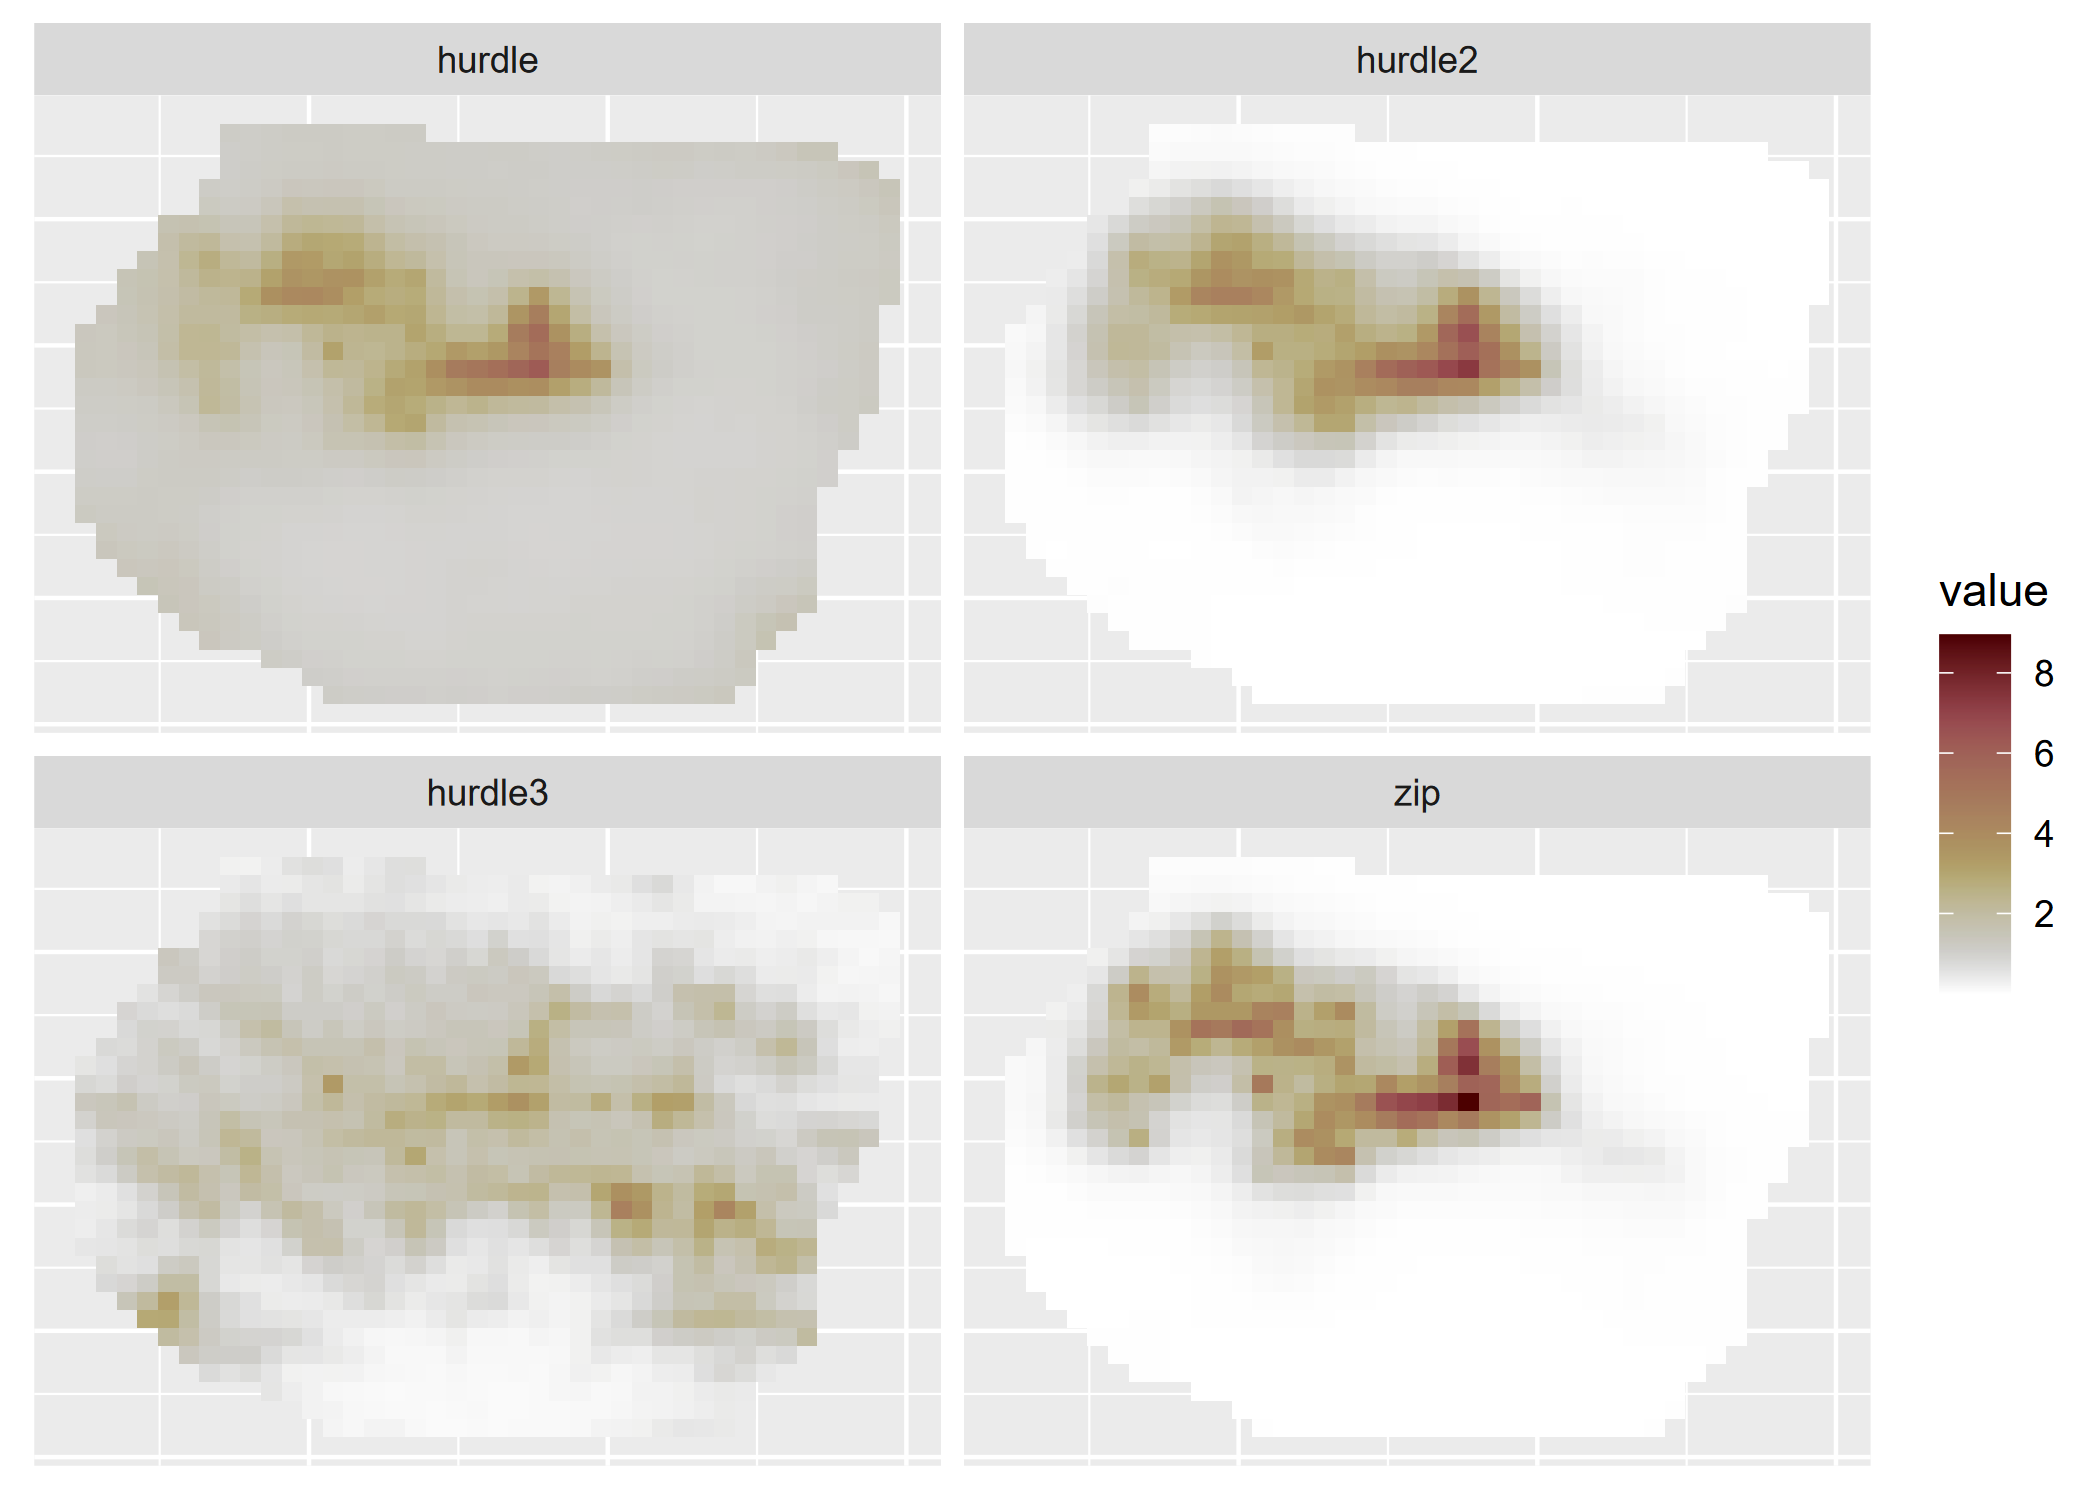
\includegraphics[keepaspectratio]{day5_practical_8_files/figure-pdf/unnamed-chunk-79-1.png}}

}

\caption{Estimated expected counts for all four models}

\end{figure}%

\begin{tcolorbox}[enhanced jigsaw, colback=white, bottomrule=.15mm, arc=.35mm, opacitybacktitle=0.6, rightrule=.15mm, breakable, coltitle=black, toprule=.15mm, bottomtitle=1mm, toptitle=1mm, titlerule=0mm, left=2mm, leftrule=.75mm, title={Task}, opacityback=0, colframe=quarto-callout-warning-color-frame, colbacktitle=quarto-callout-warning-color!10!white]

Create plots of the estimated variance of the counts.

Take hint

The fomulas for the variances are in Equation~\ref{eq-mean-zip} and
Equation~\ref{eq-mean-zap}.

Click here to see the solution

\begin{Shaded}
\begin{Highlighting}[]
\NormalTok{pred\_zip }\OtherTok{\textless{}{-}} \FunctionTok{predict}\NormalTok{(}
\NormalTok{  fit\_zip, }
\NormalTok{  counts\_df,}
  \SpecialCharTok{\textasciitilde{}}\NormalTok{ \{}
\NormalTok{    pi }\OtherTok{\textless{}{-}}\NormalTok{ zero\_probability\_parameter\_for\_zero\_inflated\_poisson\_1}
\NormalTok{    lambda }\OtherTok{\textless{}{-}}\NormalTok{ area }\SpecialCharTok{*} \FunctionTok{exp}\NormalTok{( distance }\SpecialCharTok{+}\NormalTok{ elevation }\SpecialCharTok{+}\NormalTok{ space }\SpecialCharTok{+}\NormalTok{ Intercept)}
\NormalTok{    variance }\OtherTok{\textless{}{-}}\NormalTok{ (}\DecValTok{1}\SpecialCharTok{{-}}\NormalTok{pi) }\SpecialCharTok{*}\NormalTok{ (lambda }\SpecialCharTok{+}\NormalTok{ pi }\SpecialCharTok{*}\NormalTok{ lambda}\SpecialCharTok{\^{}}\DecValTok{2}\NormalTok{)}
    \FunctionTok{list}\NormalTok{( }\AttributeTok{variance =}\NormalTok{ variance)}
\NormalTok{  \},}\AttributeTok{n.samples =} \DecValTok{2500}\NormalTok{)}

\NormalTok{pred\_zap }\OtherTok{\textless{}{-}} \FunctionTok{predict}\NormalTok{( fit\_zap, counts\_df,}
  \SpecialCharTok{\textasciitilde{}}\NormalTok{ \{}
\NormalTok{    pi }\OtherTok{\textless{}{-}}\NormalTok{ zero\_probability\_parameter\_for\_zero\_inflated\_poisson\_0}
\NormalTok{    lambda }\OtherTok{\textless{}{-}}\NormalTok{ area }\SpecialCharTok{*} \FunctionTok{exp}\NormalTok{( distance }\SpecialCharTok{+}\NormalTok{ elevation }\SpecialCharTok{+}\NormalTok{ space }\SpecialCharTok{+}\NormalTok{ Intercept)}
\NormalTok{    expect }\OtherTok{\textless{}{-}}\NormalTok{ ((}\DecValTok{1}\SpecialCharTok{{-}}\FunctionTok{exp}\NormalTok{(}\SpecialCharTok{{-}}\NormalTok{lambda))}\SpecialCharTok{\^{}}\NormalTok{(}\SpecialCharTok{{-}}\DecValTok{1}\NormalTok{) }\SpecialCharTok{*}\NormalTok{ pi }\SpecialCharTok{*}\NormalTok{ lambda)}
\NormalTok{    variance }\OtherTok{=}\NormalTok{ expect }\SpecialCharTok{*}\NormalTok{(}\DecValTok{1}\SpecialCharTok{{-}}\FunctionTok{exp}\NormalTok{(}\SpecialCharTok{{-}}\NormalTok{lambda) }\SpecialCharTok{*}\NormalTok{ expect)}
    \FunctionTok{list}\NormalTok{(}\AttributeTok{variance =}\NormalTok{ variance)}
\NormalTok{  \},}
  \AttributeTok{n.samples =} \DecValTok{2500}\NormalTok{)}

\NormalTok{inv.logit }\OtherTok{=} \ControlFlowTok{function}\NormalTok{(x) (}\FunctionTok{exp}\NormalTok{(x)}\SpecialCharTok{/}\NormalTok{(}\DecValTok{1}\SpecialCharTok{+}\FunctionTok{exp}\NormalTok{(x)))}

\NormalTok{pred\_zap2 }\OtherTok{\textless{}{-}} \FunctionTok{predict}\NormalTok{( fit\_zap2, counts\_df,}
  \SpecialCharTok{\textasciitilde{}}\NormalTok{ \{}
\NormalTok{    pi }\OtherTok{\textless{}{-}} \FunctionTok{inv.logit}\NormalTok{(Intercept\_presence }\SpecialCharTok{+}\NormalTok{ elev\_presence }\SpecialCharTok{+}\NormalTok{ dist\_presence }\SpecialCharTok{+}\NormalTok{ space\_presence)}
\NormalTok{    lambda }\OtherTok{\textless{}{-}}\NormalTok{ area }\SpecialCharTok{*} \FunctionTok{exp}\NormalTok{( dist\_count }\SpecialCharTok{+}\NormalTok{ elev\_count }\SpecialCharTok{+}\NormalTok{ space\_count }\SpecialCharTok{+}\NormalTok{ Intercept\_count)}
\NormalTok{    expect }\OtherTok{\textless{}{-}}\NormalTok{ ((}\DecValTok{1}\SpecialCharTok{{-}}\FunctionTok{exp}\NormalTok{(}\SpecialCharTok{{-}}\NormalTok{lambda))}\SpecialCharTok{\^{}}\NormalTok{(}\SpecialCharTok{{-}}\DecValTok{1}\NormalTok{) }\SpecialCharTok{*}\NormalTok{ pi }\SpecialCharTok{*}\NormalTok{ lambda)}
\NormalTok{    variance }\OtherTok{=}\NormalTok{ expect }\SpecialCharTok{*}\NormalTok{(}\DecValTok{1}\SpecialCharTok{{-}}\FunctionTok{exp}\NormalTok{(}\SpecialCharTok{{-}}\NormalTok{lambda) }\SpecialCharTok{*}\NormalTok{ expect)}
    \FunctionTok{list}\NormalTok{(}\AttributeTok{variance =}\NormalTok{ variance)}
\NormalTok{  \},}
  \AttributeTok{n.samples =} \DecValTok{2500}\NormalTok{)}

\NormalTok{pred\_zap3 }\OtherTok{\textless{}{-}} \FunctionTok{predict}\NormalTok{( fit\_zap3, counts\_df,}
  \SpecialCharTok{\textasciitilde{}}\NormalTok{ \{}
\NormalTok{    pi }\OtherTok{\textless{}{-}} \FunctionTok{inv.logit}\NormalTok{(Intercept\_presence }\SpecialCharTok{+}\NormalTok{ elev\_presence }\SpecialCharTok{+}\NormalTok{ dist\_presence }\SpecialCharTok{+}\NormalTok{ space\_copy)}
\NormalTok{    lambda }\OtherTok{\textless{}{-}}\NormalTok{ area }\SpecialCharTok{*} \FunctionTok{exp}\NormalTok{( dist\_count }\SpecialCharTok{+}\NormalTok{ elev\_count }\SpecialCharTok{+}\NormalTok{ space }\SpecialCharTok{+}\NormalTok{ Intercept\_count)}
\NormalTok{    expect }\OtherTok{\textless{}{-}}\NormalTok{ ((}\DecValTok{1}\SpecialCharTok{{-}}\FunctionTok{exp}\NormalTok{(}\SpecialCharTok{{-}}\NormalTok{lambda))}\SpecialCharTok{\^{}}\NormalTok{(}\SpecialCharTok{{-}}\DecValTok{1}\NormalTok{) }\SpecialCharTok{*}\NormalTok{ pi }\SpecialCharTok{*}\NormalTok{ lambda)}
\NormalTok{    variance }\OtherTok{=}\NormalTok{ expect }\SpecialCharTok{*}\NormalTok{(}\DecValTok{1}\SpecialCharTok{{-}}\FunctionTok{exp}\NormalTok{(}\SpecialCharTok{{-}}\NormalTok{lambda) }\SpecialCharTok{*}\NormalTok{ expect)}
    \FunctionTok{list}\NormalTok{(}\AttributeTok{variance =}\NormalTok{ variance)}
\NormalTok{  \},}
  \AttributeTok{n.samples =} \DecValTok{2500}\NormalTok{)}




  \FunctionTok{data.frame}\NormalTok{(}\AttributeTok{x =} \FunctionTok{st\_coordinates}\NormalTok{(counts\_df)[,}\DecValTok{1}\NormalTok{],}
             \AttributeTok{y =} \FunctionTok{st\_coordinates}\NormalTok{(counts\_df)[,}\DecValTok{2}\NormalTok{],}
    \AttributeTok{zip =}\NormalTok{ pred\_zip}\SpecialCharTok{$}\NormalTok{variance}\SpecialCharTok{$}\NormalTok{mean,}
         \AttributeTok{hurdle =}\NormalTok{ pred\_zap}\SpecialCharTok{$}\NormalTok{variance}\SpecialCharTok{$}\NormalTok{mean,}
         \AttributeTok{hurdle2 =}\NormalTok{ pred\_zap2}\SpecialCharTok{$}\NormalTok{variance}\SpecialCharTok{$}\NormalTok{mean,}
         \AttributeTok{hurdle3 =}\NormalTok{ pred\_zap3}\SpecialCharTok{$}\NormalTok{variance}\SpecialCharTok{$}\NormalTok{mean)  }\SpecialCharTok{\%\textgreater{}\%}
  \FunctionTok{pivot\_longer}\NormalTok{(}\SpecialCharTok{{-}}\FunctionTok{c}\NormalTok{(x,y)) }\SpecialCharTok{\%\textgreater{}\%}
  \FunctionTok{ggplot}\NormalTok{() }\SpecialCharTok{+} \FunctionTok{geom\_tile}\NormalTok{(}\FunctionTok{aes}\NormalTok{(x,y, }\AttributeTok{fill =}\NormalTok{ value)) }\SpecialCharTok{+} \FunctionTok{facet\_wrap}\NormalTok{(.}\SpecialCharTok{\textasciitilde{}}\NormalTok{name) }\SpecialCharTok{+}
\NormalTok{    theme\_map }\SpecialCharTok{+} \FunctionTok{scale\_fill\_scico}\NormalTok{(}\AttributeTok{direction =} \SpecialCharTok{{-}}\DecValTok{1}\NormalTok{)}
\end{Highlighting}
\end{Shaded}

\begin{center}
\pandocbounded{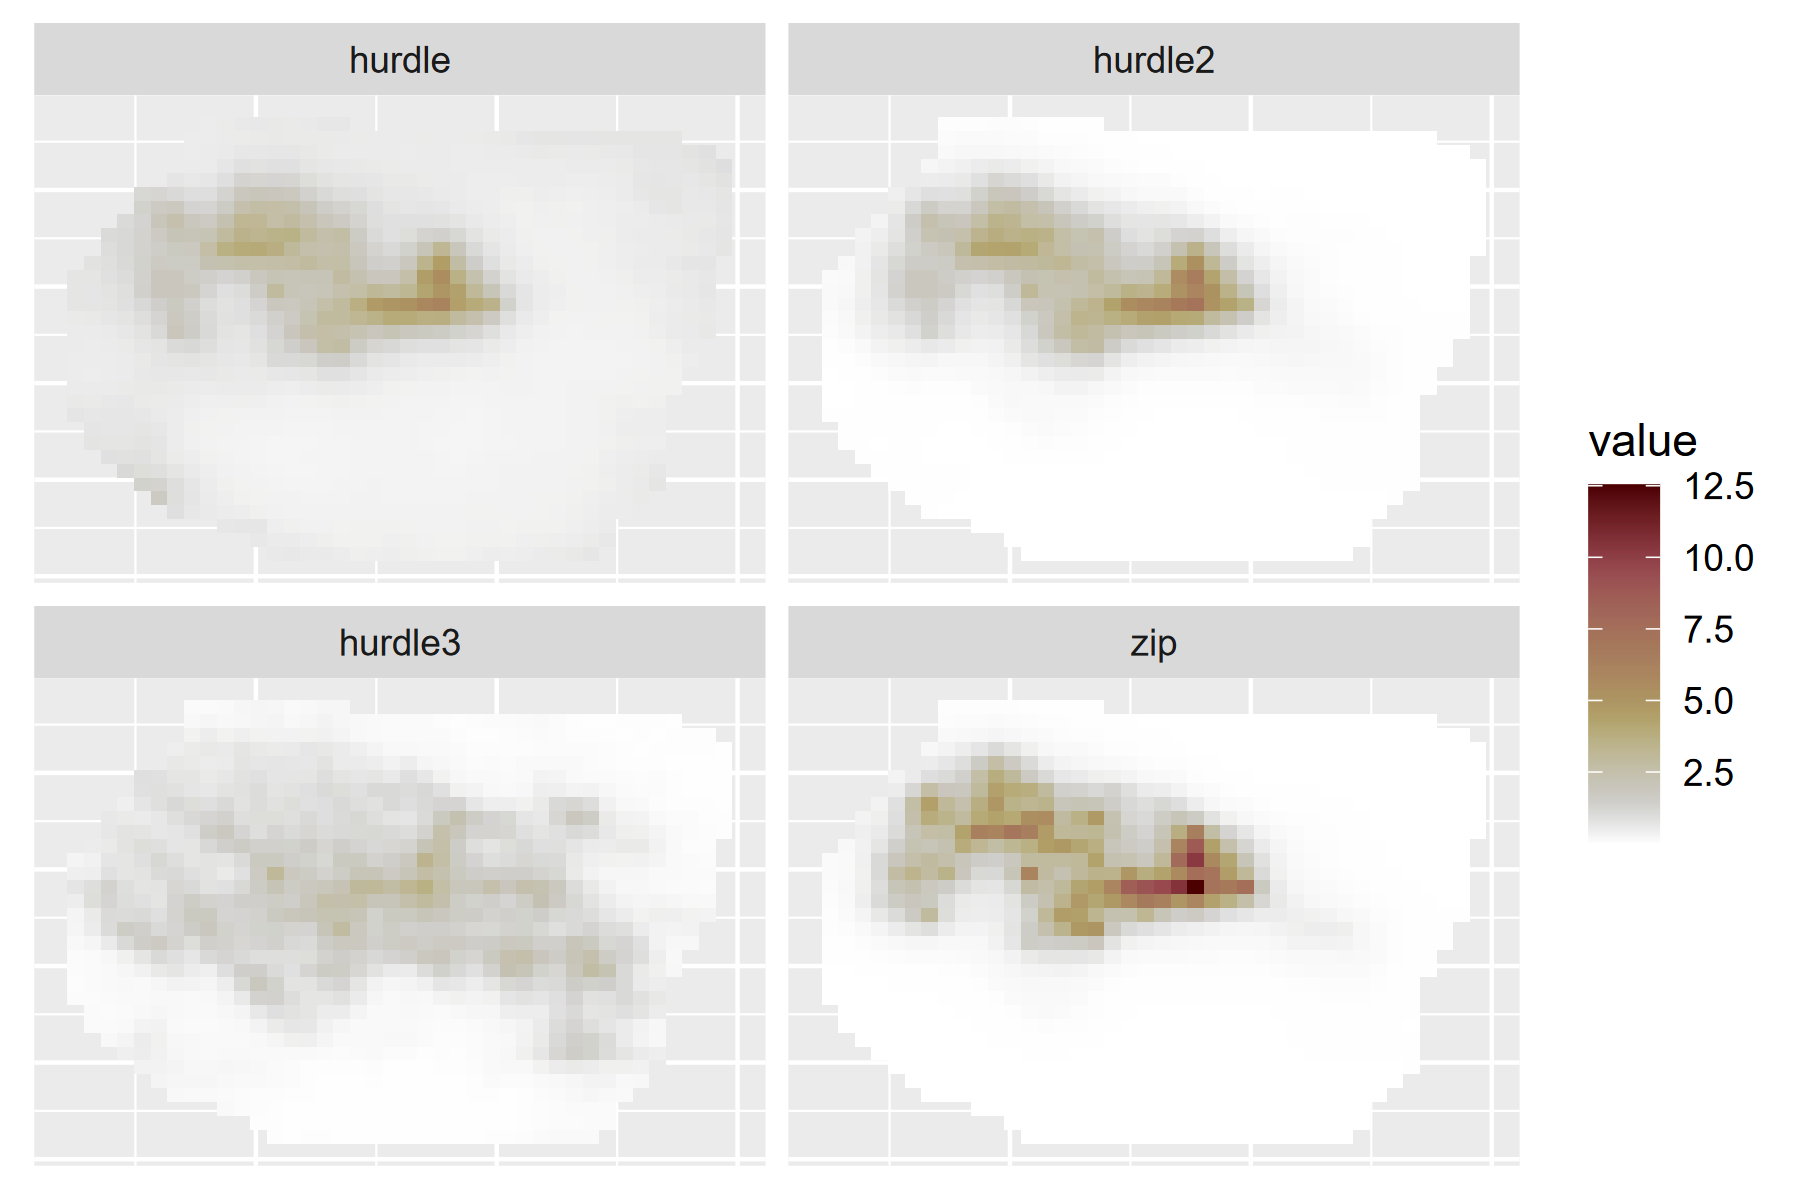
\includegraphics[keepaspectratio]{day5_practical_8_files/figure-pdf/unnamed-chunk-80-1.png}}
\end{center}

\end{tcolorbox}

\subsection{Using scores}\label{using-scores}

We can compare model using the scores that the \emph{bru()} function
computes since we have set, at the beginning. the options to :::
\{.cell\}

\begin{Shaded}
\begin{Highlighting}[]
\FunctionTok{bru\_options\_set}\NormalTok{(}\AttributeTok{control.compute =} \FunctionTok{list}\NormalTok{(}\AttributeTok{dic =} \ConstantTok{TRUE}\NormalTok{,}
                                       \AttributeTok{waic =} \ConstantTok{TRUE}\NormalTok{,}
                                       \AttributeTok{mlik =} \ConstantTok{TRUE}\NormalTok{,}
                                       \AttributeTok{cpo =} \ConstantTok{TRUE}\NormalTok{))}
\end{Highlighting}
\end{Shaded}

:::

Lets use these scores to compare the models.

\begin{tcolorbox}[enhanced jigsaw, colback=white, bottomrule=.15mm, arc=.35mm, opacitybacktitle=0.6, rightrule=.15mm, breakable, coltitle=black, toprule=.15mm, bottomtitle=1mm, toptitle=1mm, titlerule=0mm, left=2mm, leftrule=.75mm, title={Task}, opacityback=0, colframe=quarto-callout-warning-color-frame, colbacktitle=quarto-callout-warning-color!10!white]

Extract the DIC, WAIC and MLIK values for the four models and compare
them

Click here to see the solution

\begin{Shaded}
\begin{Highlighting}[]
\FunctionTok{data.frame}\NormalTok{( }\AttributeTok{Model =} \FunctionTok{c}\NormalTok{(}\StringTok{"ZIP"}\NormalTok{, }\StringTok{"HURDLE"}\NormalTok{, }\StringTok{"HURDLE\_2"}\NormalTok{,}\StringTok{"HURDLE\_3"}\NormalTok{ ),}
  \AttributeTok{DIC =} \FunctionTok{c}\NormalTok{(fit\_zip}\SpecialCharTok{$}\NormalTok{dic}\SpecialCharTok{$}\NormalTok{dic, fit\_zap}\SpecialCharTok{$}\NormalTok{dic}\SpecialCharTok{$}\NormalTok{dic, }\AttributeTok{WAIC =}\NormalTok{ fit\_zap2}\SpecialCharTok{$}\NormalTok{dic}\SpecialCharTok{$}\NormalTok{dic, fit\_zap3}\SpecialCharTok{$}\NormalTok{dic}\SpecialCharTok{$}\NormalTok{dic),}
            \AttributeTok{WAIC =} \FunctionTok{c}\NormalTok{(fit\_zip}\SpecialCharTok{$}\NormalTok{waic}\SpecialCharTok{$}\NormalTok{waic, fit\_zap}\SpecialCharTok{$}\NormalTok{waic}\SpecialCharTok{$}\NormalTok{waic, fit\_zap2}\SpecialCharTok{$}\NormalTok{waic}\SpecialCharTok{$}\NormalTok{waic, fit\_zap3}\SpecialCharTok{$}\NormalTok{waic}\SpecialCharTok{$}\NormalTok{waic),}
            \AttributeTok{MLIK =} \FunctionTok{c}\NormalTok{(fit\_zip}\SpecialCharTok{$}\NormalTok{mlik[}\DecValTok{1}\NormalTok{], fit\_zap}\SpecialCharTok{$}\NormalTok{mlik[}\DecValTok{1}\NormalTok{], fit\_zap2}\SpecialCharTok{$}\NormalTok{mlik[}\DecValTok{1}\NormalTok{], fit\_zap3}\SpecialCharTok{$}\NormalTok{mlik[}\DecValTok{1}\NormalTok{]))}
\CommentTok{\#\textgreater{}      Model      DIC     WAIC      MLIK}
\CommentTok{\#\textgreater{} 1      ZIP 1214.141 1223.721 {-}686.9496}
\CommentTok{\#\textgreater{} 2   HURDLE 1886.066 1909.722 {-}994.3807}
\CommentTok{\#\textgreater{} 3 HURDLE\_2 1268.319 1285.522 {-}734.3697}
\CommentTok{\#\textgreater{} 4 HURDLE\_3 1465.658 1515.336 {-}871.7430}
\end{Highlighting}
\end{Shaded}

\end{tcolorbox}

From the table above we can see that the model that best balances
complexity and fit is the zero inflated one (ZIP).




\end{document}
